\documentclass[handout]{beamer}
\mode<presentation> {%
	\usetheme[]{Boadilla}
	\usecolortheme{orchid}
	\setbeamercovered{transparent}
	\setbeamersize{text margin left=0.7cm}
  \setbeamersize{text margin right=0.7cm}
  \setbeamertemplate{enumerate item}[square]
  \setbeamertemplate{enumerate subitem}[circle]
  \setbeamertemplate{enumerate subsubitem}[>]
  \setbeamertemplate{itemize item}[square]
  \setbeamertemplate{itemize subitem}[circle]
  \setbeamertemplate{itemize subsubitem}[>]
}


\usepackage{pstricks}
\usepackage{pst-node}
\usepackage{bm}
\usepackage[utf8]{inputenc}
\usepackage[spanish]{babel}
\usepackage{times}
\usepackage[T1]{fontenc}
\usepackage{graphicx}
\usepackage{multirow}
\usepackage{pifont}
\usepackage{rotating}
\usepackage{colortbl}
\usepackage[framed]{mcode}
\usepackage{verbatim}
\usepackage{tikz}
\usetikzlibrary{positioning}
\usetikzlibrary{shapes.multipart,decorations.pathreplacing}
\tikzstyle{bloque}=[rectangle,rounded corners=2pt,draw=black!60,fill=black!5,very thick,minimum size=5mm,align=center]%
\tikzstyle{arrow}=[very thick,color=black!60]%


\definecolor{olivegreen}{rgb}{0.0,0.5,0.0}
\definecolor{general}{rgb}{0.9 0.9 1}%
\newrgbcolor{colorsistema}{0 1 1}
\newrgbcolor{colorviolet}{0.9 0.8 1}

\author[J. Chacón]{%[Author, Another] % (optional, use only with lots of authors)
\textit{Ingeniería Electrónica de Comunicaciones }\\
\vspace{0.6cm}
\small Jesús Chacón Sombría}%\inst{1} \and S.~Another\inst{2}}


\institute[DACYA. UCM] % (optional, but mostly needed)
{
  %\inst{1}%

\footnotesize  Departamento de Arquitectura de Computadores y Automática.\\
  Universidad Complutense de Madrid
  }

\date[Diseño de filtros] % (optional)
{\footnotesize Curso 2025-2026}%{\today / Master}
\subject{Talks}

\pgfdeclareimage[height=0.75cm]{logo}{ucm}

\usepackage[absolute,overlay]{textpos}
\setlength{\TPHorizModule}{1mm}
\setlength{\TPVertModule}{1mm}
\newcommand{\MyLogo}{%
\begin{textblock}{14}(116.0,0.6)
  \pgfuseimage{logo}
\end{textblock}
}

\makeatletter
\numberwithin{section}{part}
\AtBeginPart{
\beamer@tocsectionumber=0\relax
\frame{\partpage}
}
\makeatother

\begin{document}

\begin{frame}
  \titlepage
\end{frame}

\newcommand*\oldmacro{}%
\let\oldmacro\insertshorttitle%
\renewcommand*\insertshorttitle{%
 \MyLogo
  \oldmacro\hfill%
}

\AtBeginSection[]{}
\AtBeginSubsection[]{}

%   

%%%%%%%%%%%%%%Empieza la presentacion%%%%%%%%%%%%%%%%%%%%%%%%%%%%%%%%%%%%

%\begin{frame}
%\frametitle{Esquema}
 %   \tableofcontents
%\end{frame}

\section{Objetivos}

\begin{frame}
\frametitle{Objetivos del tema}

\begin{itemize}
\item Aprender a utilizar técnicas  de diseño de filtros generales (paso baja, paso alta, paso banda y supresor de banda):

\begin{itemize}
\normalsize
\visible<2->{
\item Continuos: 
\begin{itemize}
\small
\item Obtener únicamente la función de transferencia del filtro (no vamos a diseñar el sistema analógico que lo representa)
\item Aproximaciones a los filtros ideales
\end{itemize}
}

\visible<3->{
\item Discretos:
\begin{itemize}
\small
\item Filtros IIR: a partir de las aproximaciones de filtros continuos
\item Filtros FIR: a partir de la transformada de Fourier con ventana
\end{itemize}

}

\end{itemize}

\visible<4->{\item Aprender a diseñar filtros específicos/a medida}

\end{itemize}

\end{frame}


% \section{Introducción}

\begin{frame}\frametitle{Filtros}
    \begin{figure}
        \centering
        \small
        \begin{tikzpicture}
          \node[bloque,minimum width=15mm] (T) {H($\cdot$)};
          \node (x) [left=of T] {};
          \node (y) [right=of T] {};
          \draw[arrow,->] (x.east) -- (T.west) node [midway,above] {$x(\cdot)$};
          \draw[arrow,->] (T.east) -- (y.west) node [midway,above] {$y(\cdot)$};
        \end{tikzpicture}
    \end{figure}
    \begin{itemize}
        \item \alert{¿Qué es un filtro?}\vspace{0.1cm}
        \begin{itemize}\footnotesize
            \item<2-> Dispositivo que modifica selectivamente las frecuencias de una señal.\vspace{0.1cm}
            \item<3-> Consideramos sistemas LTI estables.\vspace{0.1cm}
            \item<4-> Caracterización mediante:
            \begin{itemize}\scriptsize
                \item<4-> Respuesta en frecuencia: \color{blue}$H(j\omega)$ \color{black} o \color{blue}$H(\textrm{e}^{j\omega})$\color{black} (continuo/discreto).\vspace{0.05cm}
                \item<4-> Respuesta impulso: \color{blue}$h(t)$ \color{black} o \color{blue}$h[n]$\color{black} (continuo/discreto).
            \end{itemize}
        \end{itemize}
    \end{itemize}
\end{frame}

\subsection{Filtros Ideales}

\begin{frame}\frametitle{Filtros Ideales}
    \begin{columns}[T]
        \begin{column}{5cm}
            \visible<1->{
                \scriptsize
                \centering{Filtro paso bajo}
                \vspace{0.1cm}
                $H(j\omega)\!=\!\left \{  \!\!\!\begin{array}{l} 1, \: \textrm{para } |\omega|\!\!<\!\!\omega_c\\0, \:\textrm{c.c.}  \end{array}\right .$
                \vspace{-0.4cm}
                \begin{figure}
                    \centering
                    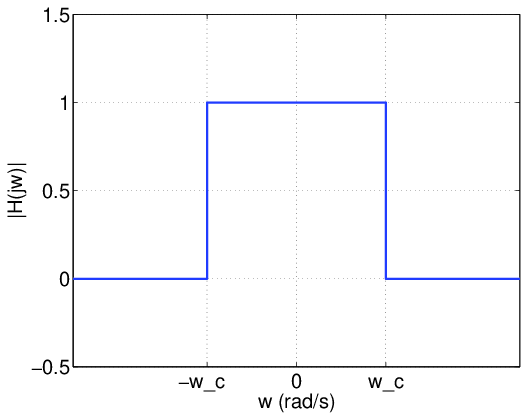
\includegraphics[width=3.2cm]{Figures/FiltroPBaja.png}
                \end{figure}
                \vspace{-0.2cm}
            }
            \visible<2->{
                \scriptsize
                \centering{Filtro paso alta}
                \vspace{0.1cm}
                $H(j\omega)\!=\!\left \{  \!\!\!\begin{array}{l} 0, \: \textrm{para } |\omega|\!\!<\!\!\omega_c\\1, \:\textrm{c.c.}  \end{array}\right .$
                \vspace{-0.4cm}
                \begin{figure}
                    \centering
                    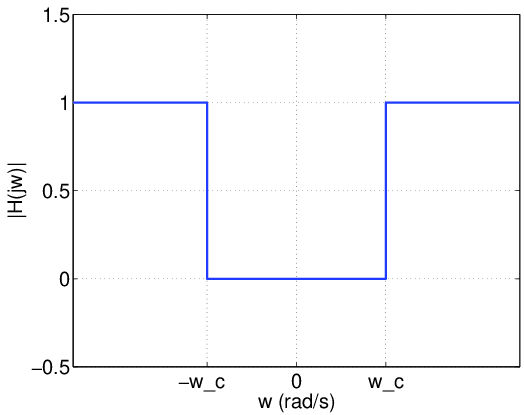
\includegraphics[width=3.2cm]{Figures/FiltroPAlta.png}
                \end{figure}
                \vspace{-0.2cm}
            }
        \end{column}
        \begin{column}{5 cm}
            \visible<3->{
                \scriptsize
                \centering{Filtro paso banda}
                \vspace{0.1cm}
                $H(j\omega)\!=\!\left \{  \!\!\!\begin{array}{l} 1, \:  \omega_{c_1}\!\!<\!\!\omega\!\!<\!\!\omega_{c_2}\\0, \:\textrm{c.c.}  \end{array}\right .$
                \vspace{-0.4cm}
                \begin{figure}
                    \centering
                    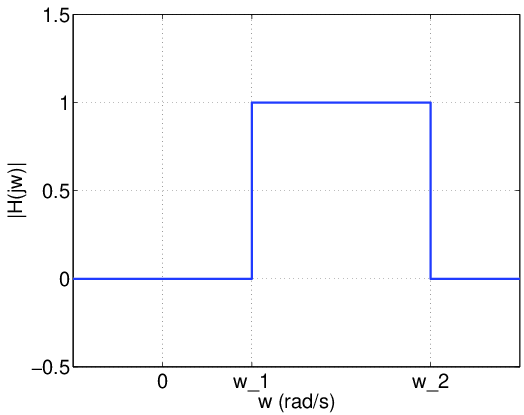
\includegraphics[width=3.2cm]{Figures/FiltroPBanda.png}
                \end{figure}
                \vspace{-0.2cm}               
            }
            \visible<4->{
                \centering{Filtro supresor banda}
                \vspace{0.1cm}
                $H(j\omega)\!=\!\left \{  \!\!\!\begin{array}{l} 0, \:  \omega_{c_1}\!\!<\!\!\omega\!\!<\!\!\omega_{c_2}\\1, \:\textrm{c.c.}  \end{array}\right .$
                \vspace{-0.4cm}
                \begin{figure}
                    \centering
                    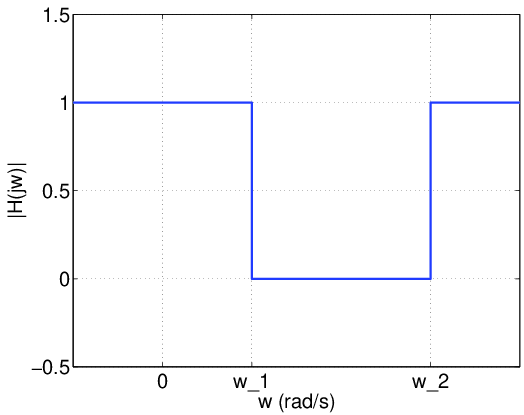
\includegraphics[width=3.2cm]{Figures/FiltroSBanda.png}
                \end{figure}
                \vspace{-0.2cm}
            }    
        \end{column}
    \end{columns}
\end{frame}
% \section{Filtros Continuos}
\subsection{Filtros continuos generales}


\begin{frame}
    \frametitle{Filtros Continuos Generales I}
    \footnotesize
    El comportamiento en frecuencia de un filtro continuo queda determinado por la posici\'{o}n de los polos y los ceros de su funci\'{o}n de transferencia $H(s)$.
    \vspace{0.1cm}
    Podemos recordar, de sistemas lineales, los comportamientos que se observan al representar la respuesta en frecuencia de diferentes filtros b\'{a}sicos (sistemas estables).
    \vspace{0.1cm}

    \begin{columns}[c]
        \hspace{0.7cm}\begin{column}{6cm}
            \alert{Polo simple}: $H(s)=\frac{a}{s+a}$, (\color{olivegreen}Ej: \color{black}a=10)
            \vspace{0.1cm}
            \scriptsize
            Atenúa, pero no totalmente.
            Si usamos varios polos simples atenuará  mas rápido.
            \vspace{0.1cm}
            \begin{figure}\centering
                \includegraphics[width=5cm]{./Figures/FiltroContinuo1b.eps}
            \end{figure}
            \vspace{-0.4cm}
        \end{column}

        \begin{column}{6cm}
            \vspace{-0.0cm}
            \alert{Cero simple: }$H(s)=\frac{s+a}{a}$, (\color{olivegreen}Ej: \color{black}a=10)
            \vspace{0.2cm}\scriptsize
            Amplifica, continuamente.
            \vspace{0.1cm}
            \begin{figure}\centering
                \includegraphics[width=5cm]{./Figures/FiltroContinuo2b.eps}
            \end{figure}
        \end{column}
    \end{columns}
\end{frame}


\begin{frame}
    \frametitle{Filtros Continuos Generales II}

    \footnotesize
    \begin{columns}[c]
        \hspace{0.7cm}\begin{column}{6cm}
            \alert{Polo doble: }$H(s)=\frac{\sigma^2+\omega_a^2}{s^2+2\sigma s +\sigma^2+\omega_a^2 }$,
            \scriptsize
            \vspace{0.1cm}
            \hspace{1.6cm}(\color{olivegreen}Ej: \color{black} $\sigma=1$, $\omega_a=3$)
            \vspace{-0.1cm}
            \begin{figure}\centering
                \includegraphics[width=3.5cm]{./Figures/FiltroContinuo3b.eps}
            \end{figure}
        \end{column}
        \begin{column}{6cm}
            \alert{Cero doble: }$H(s)=\frac{s^2+2\sigma s +\sigma^2+w_a^2 }{\sigma^2+w_a^2}$,
            \scriptsize
            \vspace{0.1cm}
            \hspace{1.6cm}(\color{olivegreen}Ej: \color{black} $\sigma=1$, $w_a=3$)
            \vspace{-0.1cm}
            \visible<2->{\begin{figure} \centering \includegraphics[width=3.5cm]{./Figures/FiltroContinuo4b.eps}  \end{figure}}
        \end{column}
    \end{columns}

    \begin{columns}[c]
        \hspace{0.7cm}\begin{column}{6cm}
        \alert{Polo doble:}$H(s)=\frac{\omega_n^2}{s^2+\omega_n^2 }$,  (\color{olivegreen}Ej: \color{black} $\omega_n=3$)
        \scriptsize
        \vspace{0.1cm}
        Es inestable para $\omega=\omega_n$
        \vspace{-0.1cm}
        \begin{figure}\centering
            \includegraphics[width=3.5cm]{./Figures/FiltroContinuo5b.eps}
        \end{figure}
    \end{column}
    \vspace{0.1cm}
    \begin{column}{6cm}
        \alert{Cero doble: }$H(s)=\frac{s^2+\omega_n^2 }{\omega_n^2}$, (\color{olivegreen}Ej: \color{black}$\omega_n=3$)
        \scriptsize
        \vspace{0.1cm}
        atenua totalmente a $\omega=\omega_n$
        \vspace{-0.1cm}
        \begin{figure}\centering
            \includegraphics[width=3.5cm]{./Figures/FiltroContinuo6b.eps}
        \end{figure}
        \end{column}
    \end{columns}
\end{frame}

%%%%%%%%%%%%%%%%%%%%%%%%%%%%%


\begin{frame}
    \frametitle{Filtros Continuos Generales III}
    \footnotesize
    Para obtener la función de transferencia de un filtro continuo podemos:
    \begin{itemize}
        \item Colocar dos ceros imaginarios puros sobre las frecuencias $\omega_n$ que deseamos eliminar completamente
        \item Compensar la amplificación asociada a cada cero, con un polo con parte real negativa (eligiendo el valor de la $a$ o de la $\omega_a$ de forma apropiada).
        \item Necesitamos al menos tantos polos como ceros que el sistema sea causal (y para atenuar la amplificación continua final asociada a cada cero).
    \end{itemize}
    Sin embargo, este método no es siempre trivial (muchos parámetros).
\end{frame}

\subsection{Filtros paso bajo}
%%%%%%%%%%%%%%%%%%%%%%%%%%%%%%%%%%%%%
\begin{frame}\frametitle{Especificación de Filtros Paso Bajo}
  \vspace{-0.25cm}
  \begin{center}
      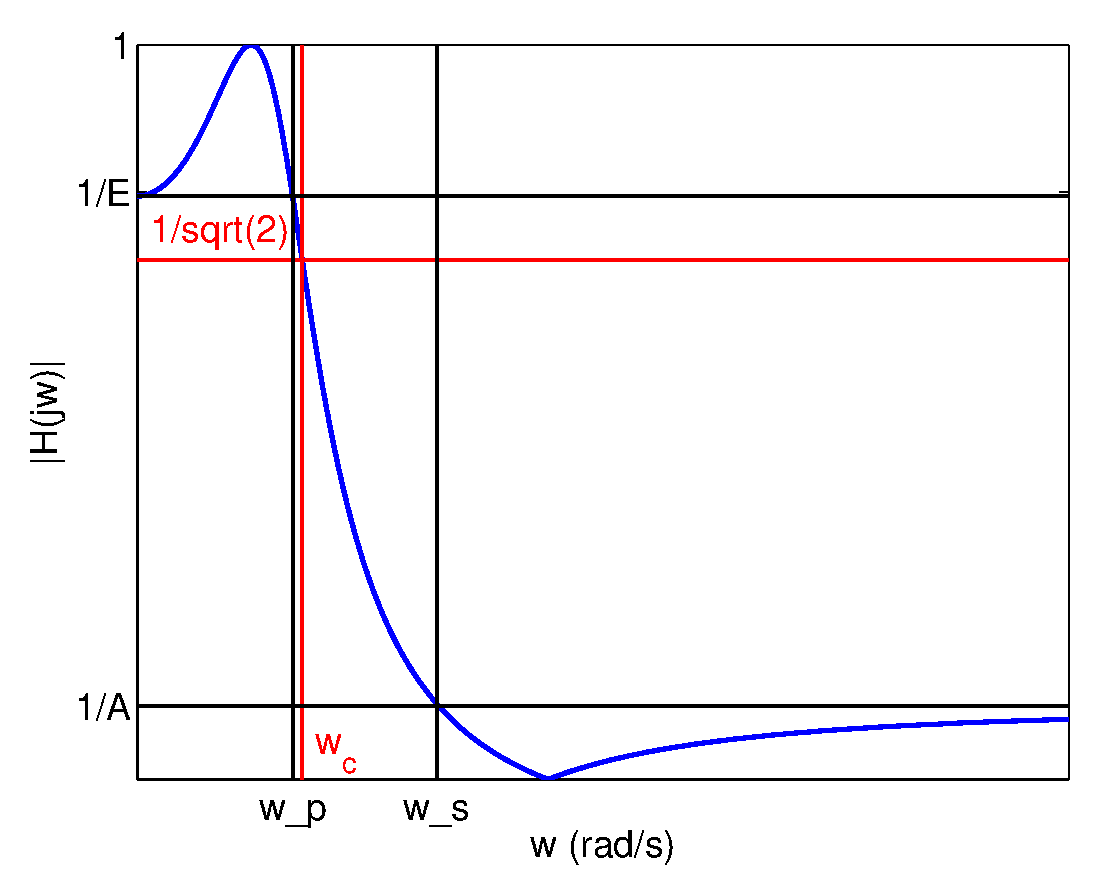
\includegraphics[width=4.8cm]{Figures/FiltroPB1_4}
  \end{center}
  \begin{alertblock}{Procedimiento de diseño}
      \begin{itemize}\small\vspace{0.05cm}
          \item Filtros paso bajo continuos con $|H(j\omega)|=\frac{1}{1+P(\omega)}$\vspace{0.05cm}
          \item $P(\omega)$ se determina de forma que $|H(j\omega)|$ se aproxime al filtro ideal\vspace{0.05cm}
          \item Para otros tipos de filtros, utilizamos transformaciones espectrales\vspace{0.05cm}
      \end{itemize}
  \end{alertblock}
\end{frame}


\begin{frame}\frametitle{Especificación de Filtros Paso Bajo}
  \begin{columns}[T]
    \begin{column}{7cm}
      \footnotesize
      \vspace{0.6cm}
          \begin{itemize}
            \scriptsize
            \item Frecuencia corte $\color{blue}\omega_c: |H(j\omega_c)|=\frac{1}{\sqrt{2}}$  (3 dB)
            \item Banda de paso: $\color{blue}[0,\omega_p]$\\
            Frecuencia paso: $\color{blue}\omega_p$\\
            Atenuación máxima banda paso (dB):
            \hspace{1cm}$\color{blue}\alpha_p=-20 \log_{10}(\frac{1}{E})$, $\color{blue}\:\:E=\sqrt{1+\epsilon^2}$
          \\
          Rizo banda paso: $\delta_p$
              \item Banda de transición: $\color{blue}[\omega_p,\omega_s]$
              \vspace{-0.1cm}
              \item Banda de supresión: $\color{blue}[\omega_s,\infty]$\\
              Frecuencia supresión: $\color{blue}\omega_s$\\
              Atenuación mínima banda supresora (dB):
              \hspace{1cm}$\color{blue}\alpha_s=-20 \log_{10}(\frac{1}{A})$\\
              \vspace{0.1cm}
              Rizo banda supresora: $\color{blue}\delta_s$
              \item Razón de transición, p. selectividad: $\color{blue}k=\frac{\omega_p}{\omega_s}$
              \item Parámetro de discriminación: $\color{blue}k_1=\frac{\epsilon}{\sqrt{A^2-1}}$
          \end{itemize}
      \end{column}
      \begin{column}{6cm}
          \footnotesize
          \hspace{1.5cm}Filtro ideal\\
          \hspace{2.1cm}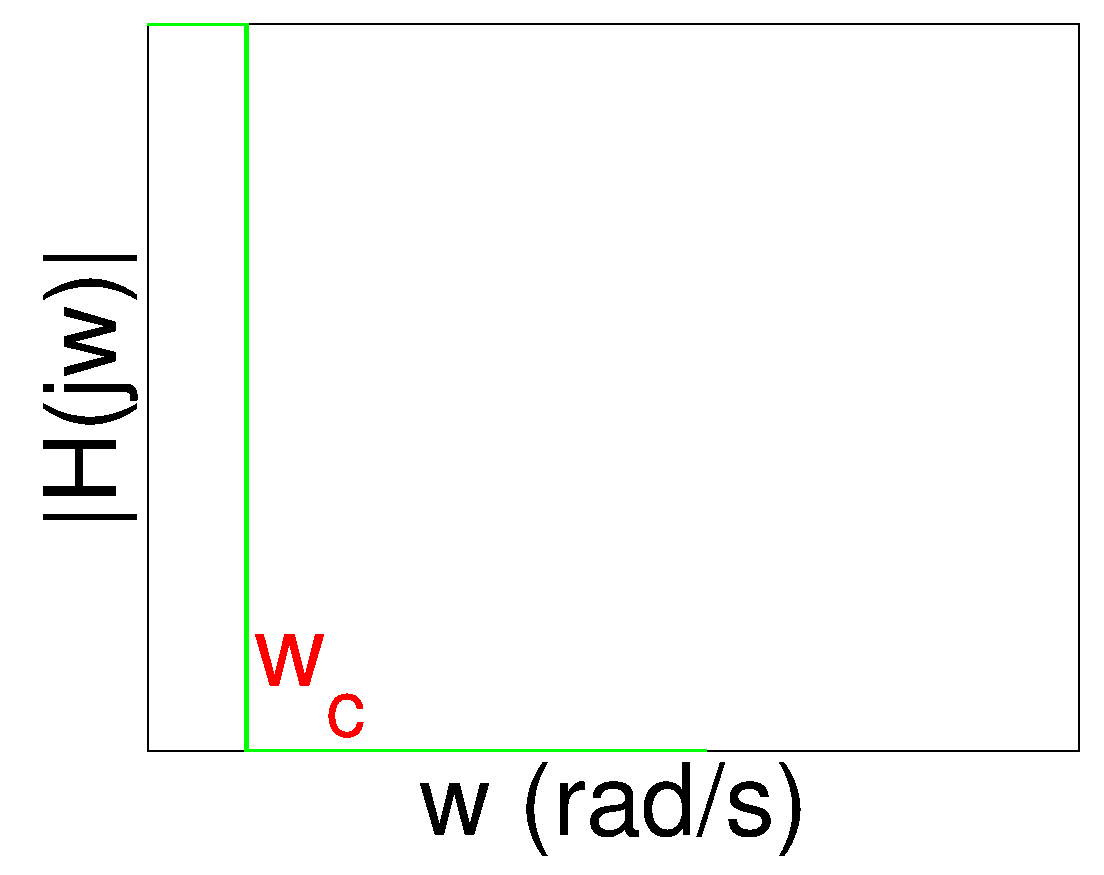
\includegraphics[width=4cm]{Figures/FiltroPB0_2}
          \hspace{3cm}Filtro real\\
          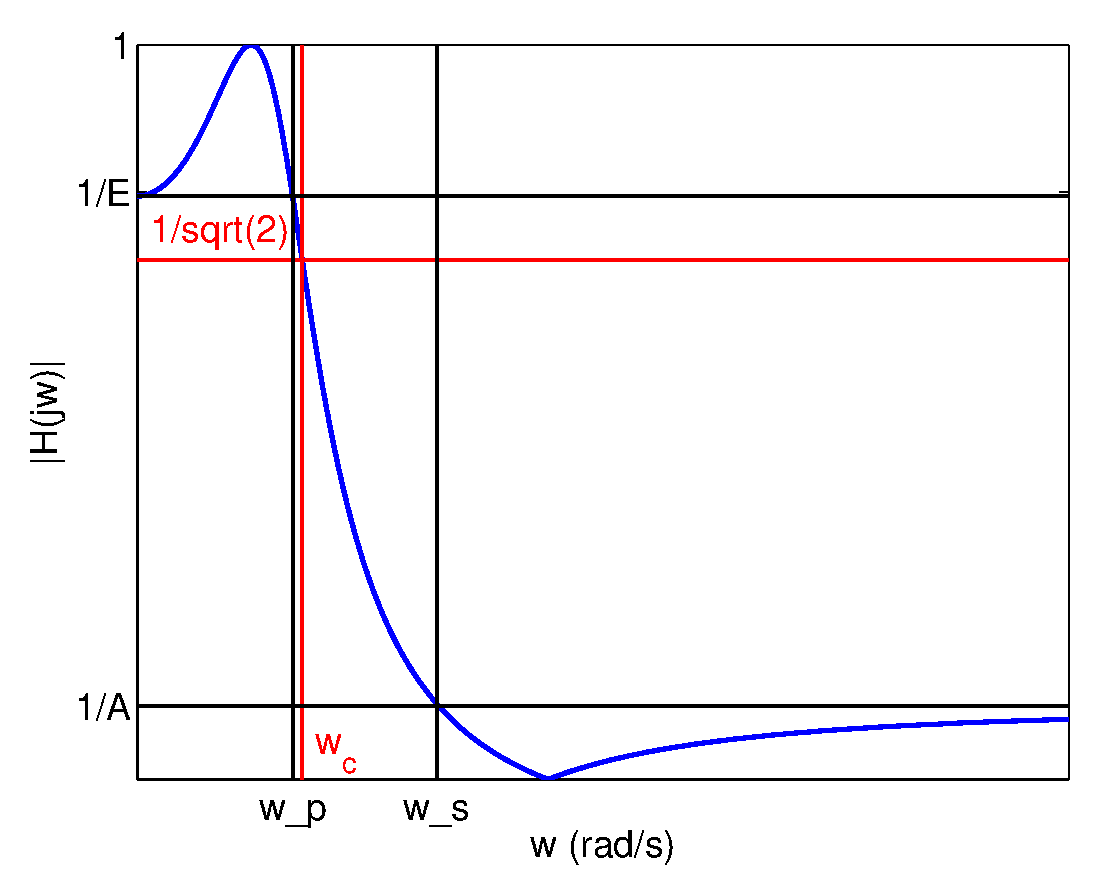
\includegraphics[width=4cm]{Figures/FiltroPB1_4}
      \end{column}
  \end{columns}
\end{frame}

\begin{frame}\frametitle{Especificación de Filtros Paso Bajo}
  \vspace{-0.9cm}
  \begin{center}
      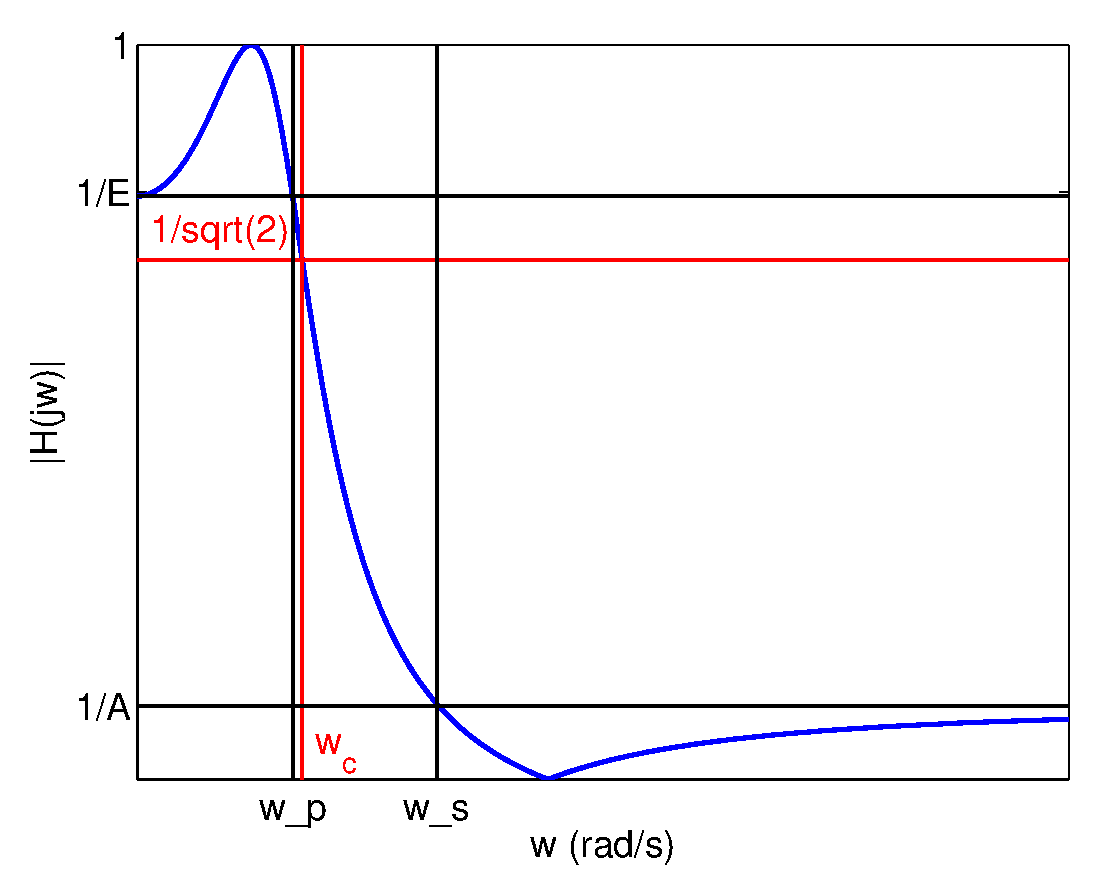
\includegraphics[width=4.8cm]{Figures/FiltroPB1_4}
  \end{center}
  \begin{alertblock}{Parámetros a especificar en un filtro paso bajo}
      \begin{itemize}
          \item $\omega_p$: Frecuencia de paso (rad/s o Hz)
          \item $\omega_s$: Frecuencia de supresión (rad/s o Hz)
          \item $\alpha_p$: Atenuación máxima en la banda de paso (dB)
          \item $\alpha_s$: Atenuación mínima en la banda de supresión (dB)
      \end{itemize}
  \end{alertblock}
\end{frame}

\begin{frame}\frametitle{Algunos tipos de filtros paso bajo}
  \begin{columns}[T]
      \hspace{-0.2cm}\begin{column}{4cm}
          \scriptsize
          \visible<2->{
              \hspace{1.5cm}Butterworth
              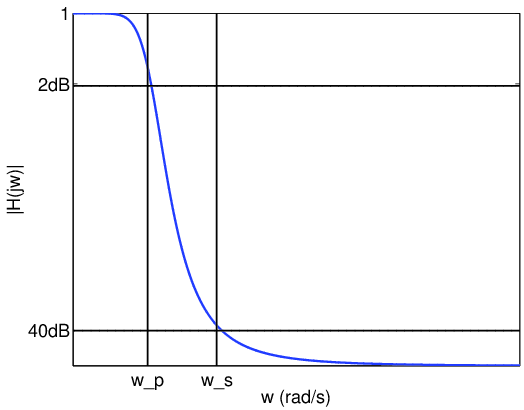
\includegraphics[width=4cm]{Figures/FiltroPB2_Butter.png}
          }
          \visible<4->{
              \hspace{1.5cm}Chebyshev I
              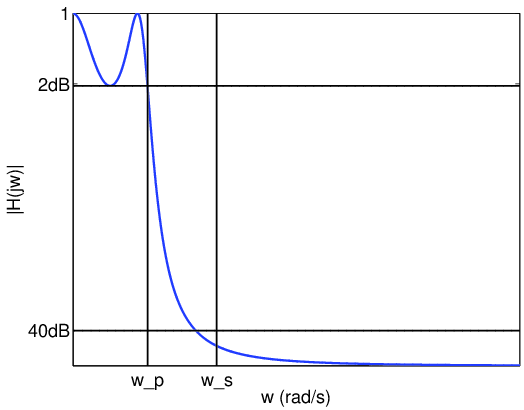
\includegraphics[width=4cm]{Figures/FiltroPB2_Cheby1.png}
          }
      \end{column}
      \hspace{-0.2cm}\begin{column}{4cm}
          \scriptsize
          \visible<2->{
              \hspace{1.9cm}Eliptico
              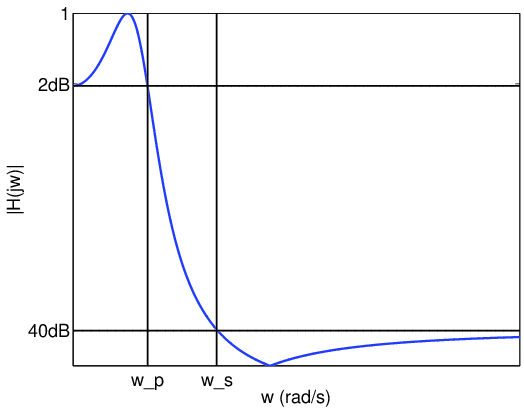
\includegraphics[width=4cm]{Figures/FiltroPB2_Ellip.png}
          }
          \visible<4->{
              \hspace{1.4cm}Chebyshev II
              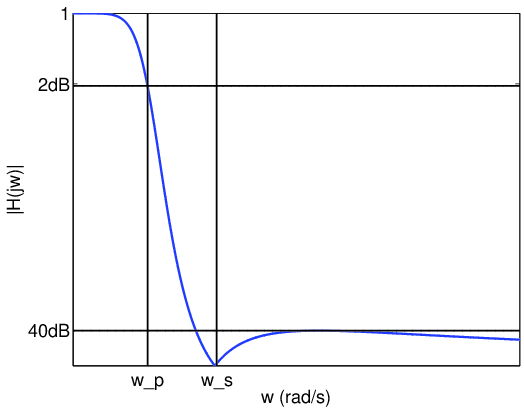
\includegraphics[width=4cm]{Figures/FiltroPB2_Cheby2.png}
          }
          \footnotesize
      \end{column}
      \hspace{-0.3cm}\begin{column}{4.6cm}
      \footnotesize
      \visible<3->{
          \hspace{0.3cm} Diferencias:
          \vspace{-0.1cm}
          \begin{itemize}
              \item Rizado:\\
              {\scriptsize
                  \color{blue}$\star$ Butterworth\color{black}:\\ \hspace{0.5cm} Sin rizado\\
                  \color{blue}$\star$ Elíptico\color{black}:\\ \hspace{0.5cm} Dos bandas\\
              }
          \scriptsize
      }
      \visible<4->{
          \color{blue}$\star$ Chebyshev I\color{black}: \\ \hspace{0.5cm}Banda paso\\
          \color{blue}$\star$ Chebyshev II\color{black}: \\\hspace{0.5cm}Banda supresión
      }

      \visible<5->{

          \item Función Transferencia:

          {\scriptsize
          \color{blue}$\star$ \color{black} Posición de los polos/ceros\\
          \color{blue}$\star$ \color{black} Orden (\# polos)\\
          \visible<6->{
              \color{blue}$\star$ \color{black} Banda de transición (para un mismo orden):\\
              \hspace{0.2cm} \color{blue}Butterworth\color{black}:\\ \hspace{0.5cm}caída lenta\\
              \hspace{0.2cm} \color{blue}Eliptico\color{black}:\\ \hspace{0.5cm}caída rápida\\
              \hspace{0.2cm} \color{blue}Chebyshev I\color{black}: \\ \hspace{0.5cm} caída rápida paso\\
              \hspace{0.2cm} \color{blue}Chebyshev II\color{black}:\\ \hspace{0.5cm} caída rápida supresión\\
          }
      }
  }

  \end{itemize}
  \end{column}

\end{columns}


\end{frame}


%%%%%%%%%%%%%%%%%%%%%%%%%%%%%%%%

\begin{frame}
\frametitle{Filtro de Butterworth}

\begin{columns}[T]
\hspace{-0.5cm}\begin{column}{8cm}

\footnotesize


\alert{\hspace{0.3cm}$\displaystyle |H(j\omega)|^2=\frac{1}{1+\left (\frac{\omega}{\omega_c}\right )^{2N}}$}

\visible<2->{

\hspace{0.3cm}\alert{$\displaystyle  H(s)=\frac{\omega_c^N}{\prod_{l=1}^N (s-p_l)}$}, con \alert{$\displaystyle p_l=\omega_c e^{\frac{j\pi(N+2l-1)}{2N}}$}}

\vspace{0.1cm}


\vspace{-0.1cm}

\visible<4->{
\begin{itemize}
\item Para una $\omega_c$ fija,
si aumenta $N$ disminuye ancho banda de transición.

\visible<5->{
\item Dados unos valores $\omega_p$, $\omega_s$, $\alpha_p$, $\alpha_s$, determinar el filtro de menor $N$ que los cumple (fijando $\omega_c$).
}

\color{gray}

\scriptsize

\visible<6->{
  $\!\!\!\!\left . \begin{array}{l}
\alpha_p=-20 log_{10} \frac{1}{E} \\ \alpha_s=-20 log_{10} \frac{1}{A}\end{array}\right \}$ }   \visible<7->{ $\rightarrow \displaystyle\left . \begin{array}{l}
E= 10^{\frac{ \alpha_p}{20}} \\ A=10^{\frac{ \alpha_s}{20}} \end{array}\right \}$}

\end{itemize}
}

\end{column}
\hspace{-0.3cm}\begin{column}{4cm}
\visible<1->{
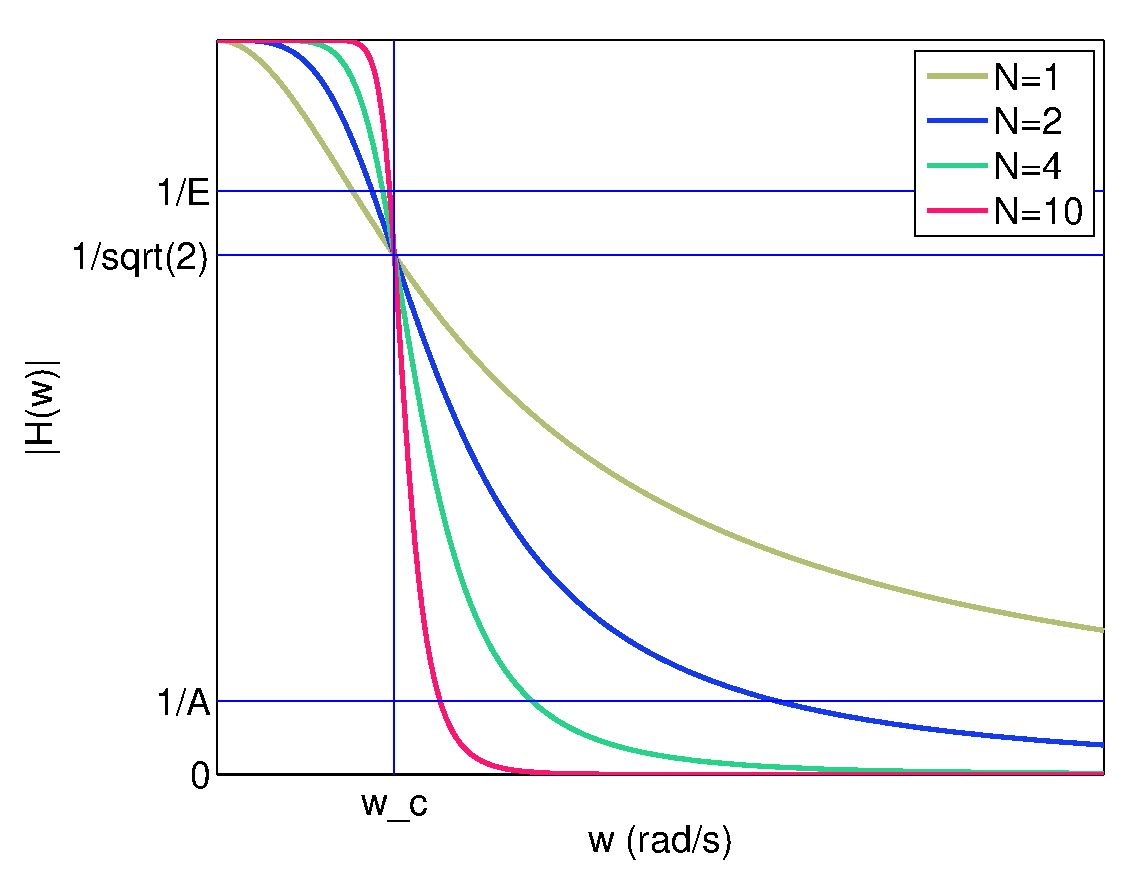
\includegraphics[width=3.5cm]{Figures/FiltroPB_Butter}
}

\vspace{0.1cm}

\visible<3->{
\hspace{0.8cm}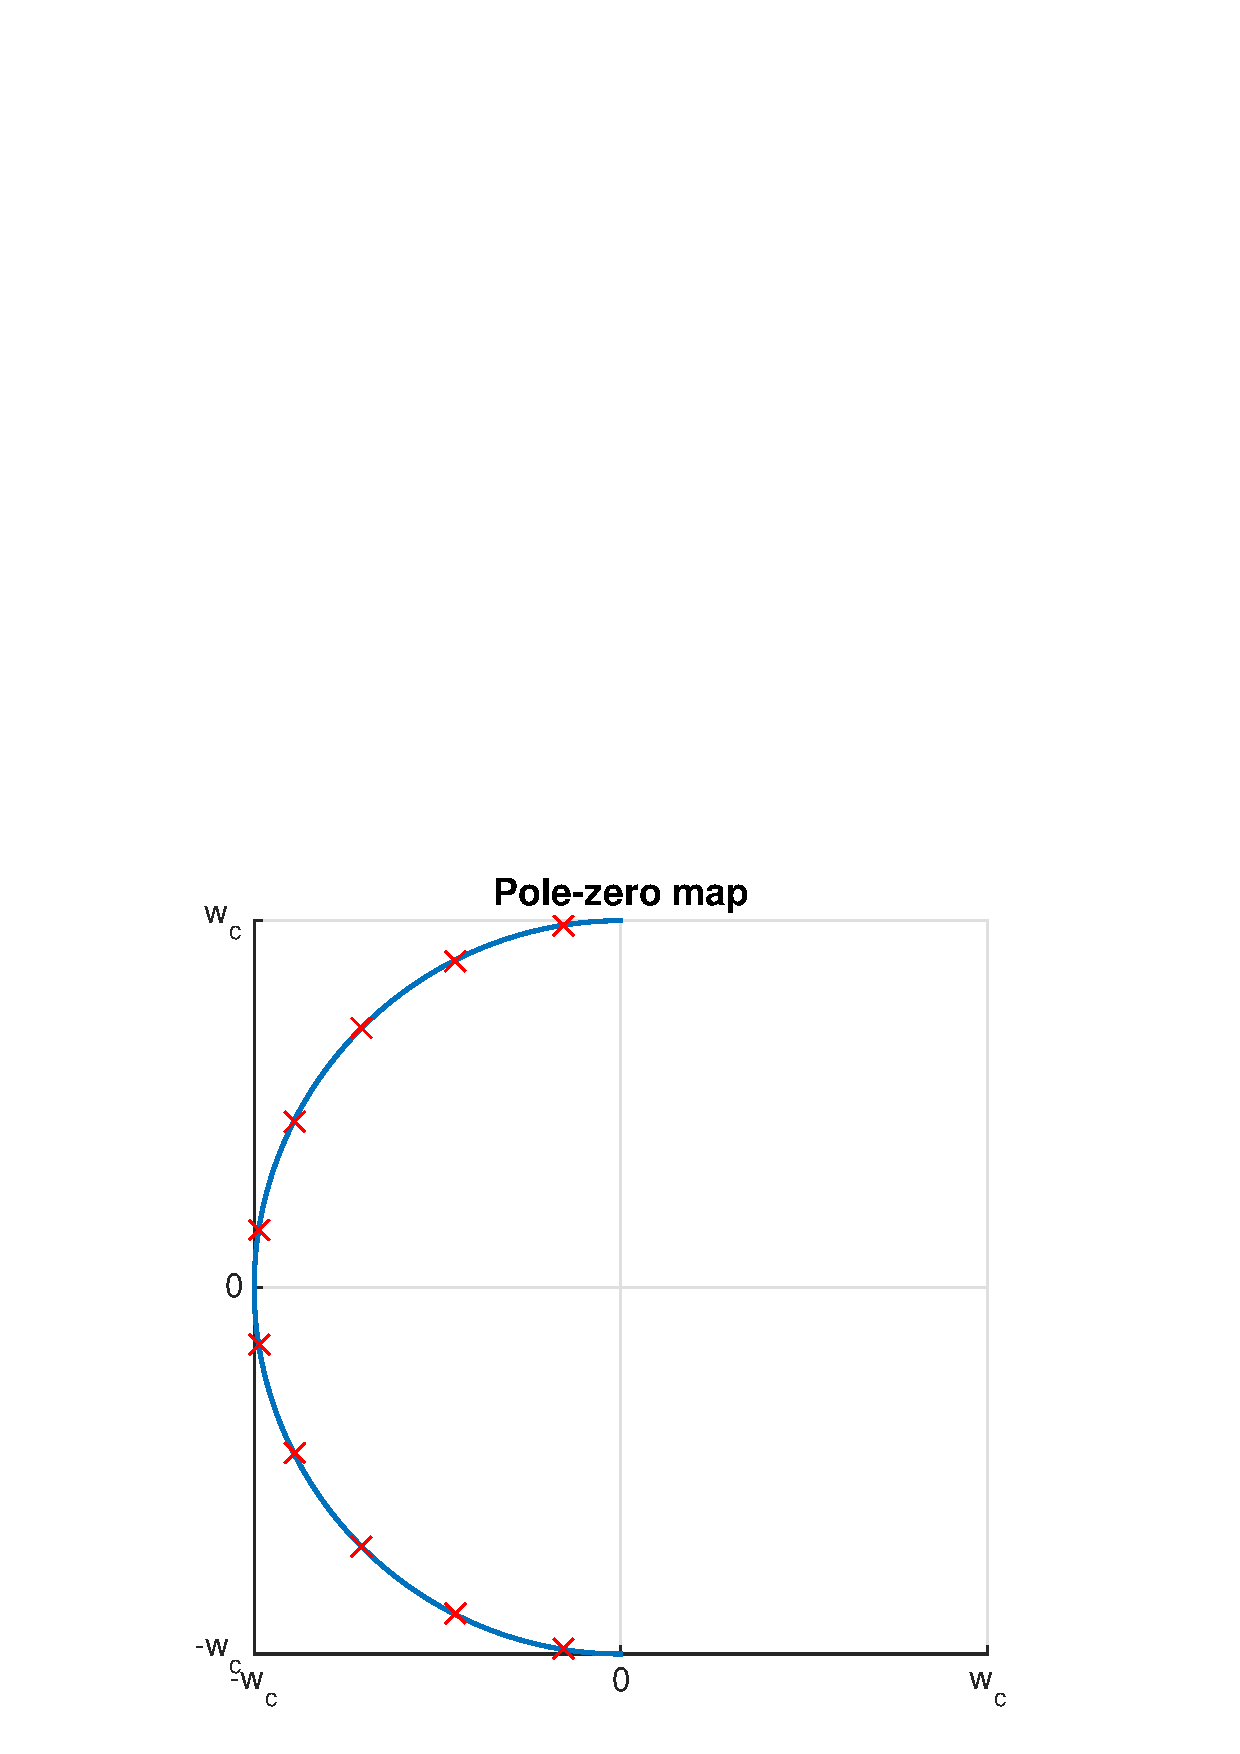
\includegraphics[width=2.2cm]{Figures/PolesButter}
}

\end{column}
\end{columns}

\vspace{-0.1cm}



{

\scriptsize
\color{gray}


\visible<6->{
\hspace{0.0cm} $\!\!\!\!\left . \begin{array}{l}|H(j\omega_p)|^2=\frac{1}{1+\left (\frac{\omega_p}{\omega_c}\right )^{2N}}=\frac{1}{E^2} \\
|H(j\omega_s)|^2=\frac{1}{1+\left (\frac{\omega_s}{\omega_c}\right )^{2N}}=\frac{1}{A^2}\\
\end{array}\right \}  $}   \visible<8->{$\rightarrow \!\!\left . \begin{array}{l}E^2-1=\left (\frac{\omega_p}{\omega_c}\right )^{2N} \\
A^2-1=\left (\frac{\omega_s}{\omega_c}\right )^{2N} \\
\end{array}\right \}\rightarrow $ $ \frac{A^2-1}{E^2-1}=\left (\frac{\omega_s}{\omega_p}\right )^{2N} \rightarrow $

\vspace{-.1cm}
\hspace{0.0cm}   $log_{10} \frac{A^2-1}{E^2-1}=2N log_{10}\frac{\omega_s}{\omega_p}\rightarrow$ $\alert{N=\frac{1}{2}\frac{log_{10} \frac{A^2-1}{E^2-1}}{log_{10}\frac{\omega_s}{\omega_p}}} \rightarrow$  $N=\frac{log_{10} \frac{1}{k_1}}{log_{10}\frac{1}{k}} $
}

\visible<9>{
\hspace{0.0cm}  $A^2-1=\left (\frac{\omega_s}{\omega_c}\right )^{2N}\rightarrow$  $\omega_c^{2N}=\frac{\omega_s^{2N}}{A^2-1} \rightarrow$     \alert{$\omega_c=\frac{\omega_s}{(A^2-1)^{\frac{1}{2N}}}$}
}

}

\end{frame}


%%%%%%%%%%%%%%%%%%%%%%%%%%%%%%%

\begin{frame}
\frametitle{Filtro de Butterworth (ejemplo)}

\begin{itemize}

{
\scriptsize
\item \color{olivegreen} Determinar el filtro de Butterworth de orden más bajo con una atenuación en la banda de paso máxima de 1dB a 1KHz y una atenuación mínima en la banda de supresión de 40dB a 5KHz.

\begin{columns}[T]
\hspace{0.8cm}\begin{column}{7.1cm}
\color{gray}

\visible<2->{

 $\begin{array}{l}\!\!\!\left .\begin{array}{l}\omega_p=2\pi*1000\\
 \omega_s=2\pi*5000\\
 \alpha_p=1dB\\
 \alpha_s=40\end{array}\!\!\!\right \} \rightarrow\\ \: \\ \: \end{array}$ } \visible<3->{$\!\!\!\!\!\!\begin{array}{l}E= 10^{\frac{ \alpha_p}{20}}=1.122 \\ A=10^{\frac{ \alpha_s}{20}}=100\\
 N\!=\!\frac{1}{2}\frac{log_{10} \frac{A^2-1}{E^2-1}}{log_{10}\frac{\omega_s}{\omega_p}} \!=\!3.28 \rightarrow 4 \\
 \omega_c=\frac{\omega_s}{(A^2-1)^{\frac{1}{2N}}}\approx 9935 \end{array}$}
 \end{column}
\hspace{-1cm} \begin{column}{4cm}
\vspace{-0.2cm}
\visible<4->{ 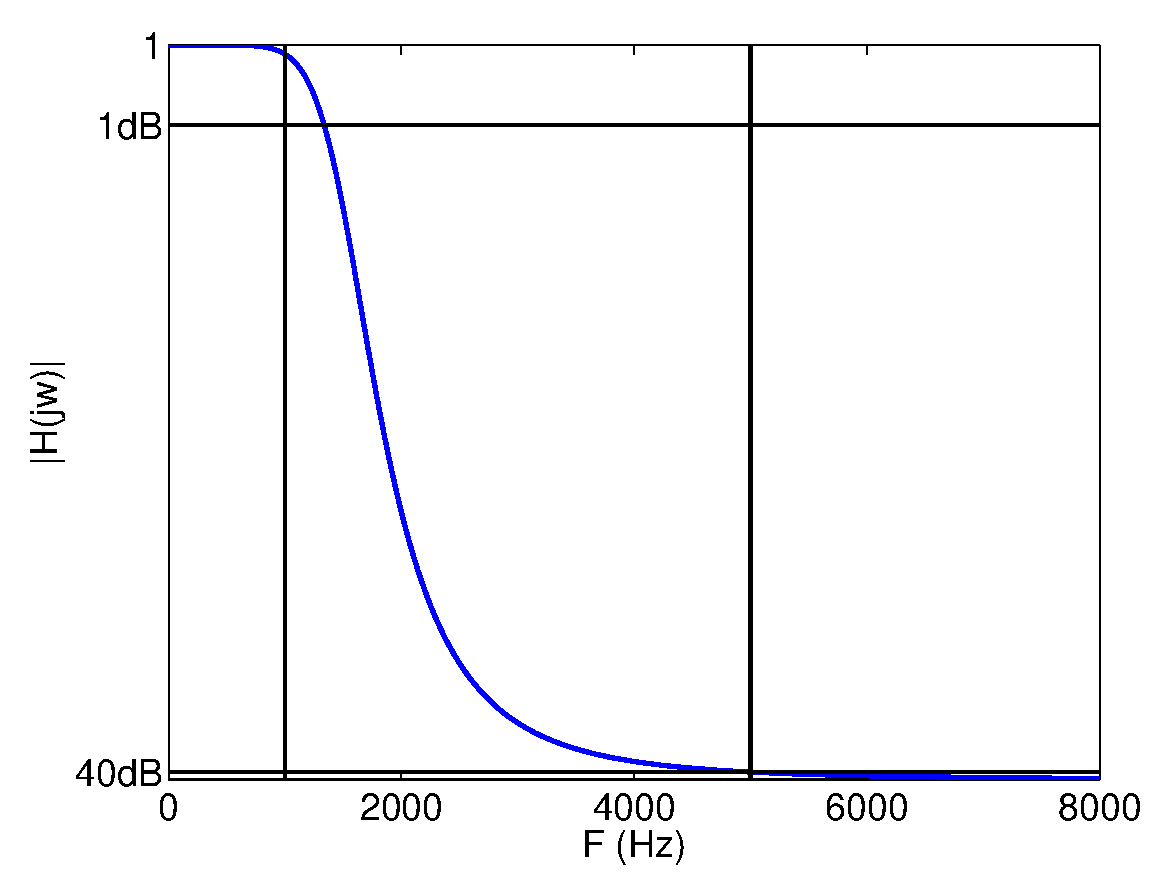
\includegraphics[width=4cm]{./Figures/FiltroPB_ButterEx.eps}}
 \end{column}
 \end{columns}

}
\visible<5->{
{

\vspace{-0.5cm}

\footnotesize
\item Con Matlab:

\begin{itemize}
\item \alert{\texttt{[N,wc]=buttord(wp,ws,ap,as,'s')}}
\begin{itemize}
\color{gray}
\item Calcula el orden \texttt{N} del filtro y la frecuencia de corte \texttt{wc}.
\item \texttt{wp}, \texttt{ws} en rad/s.
\item \texttt{ap}, \texttt{as} en dB.
\item 's' para que calcule los valores del filtro de continuo.
\end{itemize}
\item \alert{\texttt{[B,A]=butter(N,wc,'low','s')}}
\begin{itemize}
\color{gray}
\item Calcula el numerador y denominador de $H(s)$.
\end{itemize}
\item \alert{\texttt{[Hw,w]=freqs(B,A)}}
\begin{itemize}
\color{gray}
\item Calcula la $H(j\omega)$ del filtro para las frecuencias \texttt{w}.
\end{itemize}

\end{itemize}
}
}
\end{itemize}

\end{frame}

%%%%%%%%%%%%%%%%%%%%%%%%%%%%%%%%%%%%%%

\begin{frame}
\frametitle{Filtro de Chebyshev Tipo I}

\begin{columns}[T]
\hspace{0.4cm}\begin{column}{8cm}

\footnotesize

\footnotesize


\hspace{0.4cm}\alert{$\displaystyle |H(j\omega)|^2=\frac{1}{1+\epsilon^2 T_N^2(\omega/\omega_p)}$}

\vspace{0.1cm}

\hspace{0.4cm}$T_N(w)=\left \{ \begin{array}{l}cos(N \cdot acos(\omega)) \:\:\:\:\:\:\:\: |\omega|\le 1\\ cosh(N \cdot acosh(\omega)) \:\:\: |\omega|> 1\end{array} \right .$

\visible<2->{

\hspace{0.4cm}\alert{$\displaystyle  H(s)=\frac{K_N}{\prod_{l=1}^N (s-p_l)}$}, con \alert{$\displaystyle p_l=\sigma_l+j\omega_l$}

\vspace{0.1cm}

\hspace{0.4cm}$\sigma_l=-\omega_p \frac{\gamma^2-1}{2\gamma}sin\left( \frac{(2l-1)\pi}{2N}\right)$, \hspace{0.5cm}$\gamma=\left ( \frac{1+\sqrt{1+\epsilon^2}}{\epsilon} \right )^{\frac{1}{N}}$

\vspace{0.1cm}

\hspace{0.4cm}$\omega_l= \omega_p \frac{\gamma^2+1}{2\gamma}cos\left( \frac{(2l-1)\pi}{2N}\right)$, \hspace{0.5cm}$E=\sqrt{1+\epsilon^2}$}


\vspace{-0.1cm}

\begin{itemize}

\visible<4->{

\item Para una $\omega_p$ fija,
si aumenta $N$ disminuye ancho de la banda de transición.


}
\end{itemize}




\end{column}
\hspace{-0.5cm}\begin{column}{4cm}
\visible<1->{
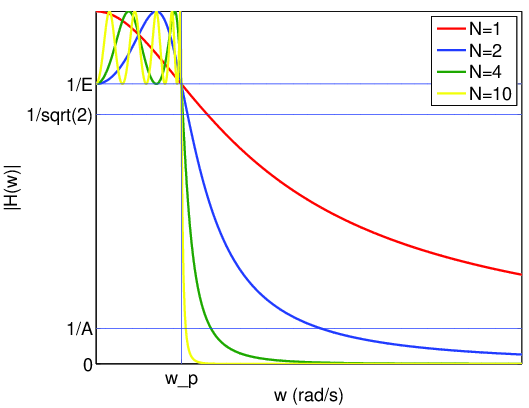
\includegraphics[width=3.5cm]{Figures/FiltroPB_Cheby1.png}
}

\vspace{0.1cm}


\visible<3->{
\hspace{0.8cm}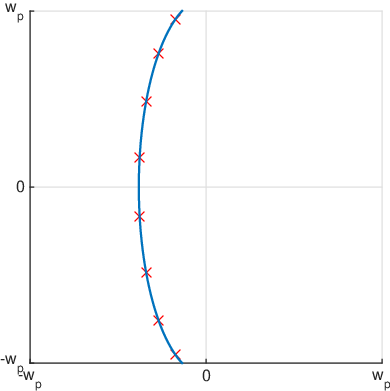
\includegraphics[width=2.2cm]{Figures/PolesCheby1.png}
}

\end{column}
\end{columns}

\vspace{0.1cm}

\footnotesize
\begin{itemize}



\visible<5->{
\item Determinar el filtro de menor $N$ para valores dados de  $\omega_p$, $\omega_s$, $\alpha_p$, $\alpha_s$.
}
\vspace{0.1cm}
{

\color{gray}

\scriptsize

  $\!\!\!\!\left . \begin{array}{l}
\alpha_p=-20 log_{10} \frac{1}{E} \\ \alpha_s=-20 log_{10} \frac{1}{A}\end{array}\right \}$ }   \visible<7->{ $\rightarrow \displaystyle\left . \begin{array}{l}
E= 10^{\frac{ \alpha_p}{20}} \\ A=10^{\frac{ \alpha_s}{20}} \end{array}\right \}$ $\rightarrow \epsilon=\sqrt{E^2-1}$ }

\vspace{-0.3cm}

\visible<6->{
$
|H(j\omega_s)|^2=\frac{1}{1+\epsilon^2 cosh^2( N\cdot acosh(\omega_s/\omega_p))}=\frac{1}{A^2} \rightarrow$}   \visible<8->{\alert{$
N=\frac{acosh \left ( \frac{\sqrt{A^2-1}}{\epsilon} \right)}{acosh(\omega_s/\omega_p)} $} $\rightarrow N=\frac{acosh \frac{1}{k_1}}{acosh\frac{1}{k}} $
}


\end{itemize}
\end{frame}

%%%%%%%%%%%%%%%%%%%%%%%%%%%%%%%

\begin{frame}
  \frametitle{Filtro de Chebyshev Tipo I (ejemplo)}
  
  \begin{itemize}
    
    \scriptsize
    \item \color{olivegreen} Determinar el filtro de Chebyshev tipo I de orden más bajo con una atenuación en la banda de paso máxima de 1dB a 1KHz y una atenuación mínima en la banda de supresión de 40dB a 5KHz.
    
    \begin{columns}[T]
      \hspace{0.7cm}\begin{column}{7.1cm}
      \color{gray}
      {$\begin{array}{l}\!\!\!\left .\begin{array}{l}
        \omega_p=2\pi\cdot 1000\\
        \omega_s=2\pi\cdot 5000\\
        \alpha_p=1dB\\
        \alpha_s=40\end{array}\!\!\!\right \} \rightarrow\\ \: \\ \: \end{array}$ } \visible<2->{$\!\!\!\!\!\!\begin{array}{l}E= 10^{\frac{ \alpha_p}{20}}=1.122 \\ A=10^{\frac{ \alpha_s}{20}}=100\\ \epsilon=\sqrt{E^2-1}=0.5088 \\
        N\!=\!\frac{acosh \!\left (\! \frac{\sqrt{A^2-1}}{\epsilon}\! \right)}{acosh(\omega_s/\omega_p)} \!=\!2.61 \rightarrow 3 \end{array}$}
      \end{column}
      \hspace{-0.9cm} \begin{column}{4cm}
        \vspace{-0.2cm}
        \visible<3->{ 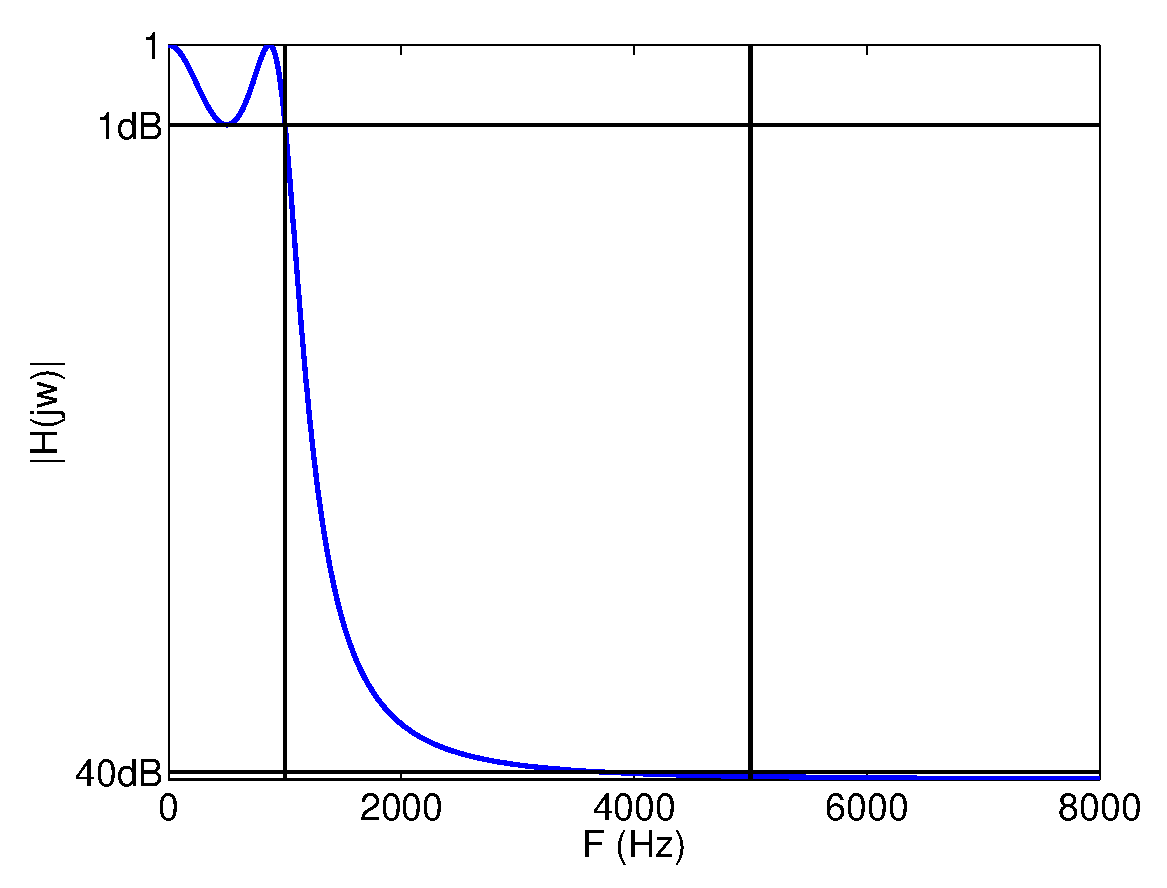
\includegraphics[width=4cm]{./Figures/FiltroPB_Cheby1Ex.eps}}
      \end{column}
    \end{columns}
  
    \vspace{-0.5cm}
    
    \footnotesize
    \item Con Matlab:
    
    \begin{itemize}
      \item \alert{\texttt{[N,wc]=cheb1ord(wp,ws,ap,as,'s')}}
      \begin{itemize}
        \color{gray}
        \item Calcula el orden \texttt{N} del filtro y la frecuencia de corte \texttt{wc}.
        \item \texttt{wp}, \texttt{ws} en rad/s.
        \item \texttt{ap}, \texttt{as} en dB.
        \item 's' para que calcule los valores del filtro de continuo.
      \end{itemize}
      \item \alert{\texttt{[B,A]=cheby1(N,ap,wc,'low','s')}}
      \begin{itemize}
        \color{gray}
        \item Calcula el numerador \texttt{B} y denominador \texttt{A} de $H(s)$
      \end{itemize}
      \item \alert{\texttt{[Hw,w]=freqs(B,A)}}
      \begin{itemize}
        \color{gray}
        \item Calcula la $H(j\omega)$ del filtro, \texttt{Hw}, para las frecuencias \texttt{w}
      \end{itemize}
        
    \end{itemize}
    
  \end{itemize}
\end{frame}
  
  
  %%%%%%%%%%%%%%%%%%%%%%%%%%%%%%%%%%%%
  
  
  \begin{frame}
  \frametitle{Filtro de Chebyshev Tipo II}
  
   \vspace{-0.2cm}
  
  \begin{columns}[T]
  \hspace{0.3cm}\begin{column}{8cm}
  
  \footnotesize
  
  \visible<1->{
  
  \hspace{0.4cm}\alert{$\displaystyle |H(jw)|^2=\frac{1}{1+\epsilon^2 \frac{T_N^2(\omega_s/\omega_p)}{T_N^2(\omega_s/w)}}$}
  
  \hspace{0.4cm}$T_N(w)=\left \{ \begin{array}{l}cos(N \cdot acos(w)) \:\:\:\:\:\:\:\: |w|\le 1\\ cosh(N \cdot acosh(w)) \:\:\: |w|> 1\end{array} \right .$
  
  }
  
  \visible<2->{
  
  \hspace{0.4cm}\alert{$\displaystyle  H(s)=C_0\frac{\prod_{l=1}^N (s-z_l)}{\prod_{l=N+1}^{2N} (s-p_l)}$}, con \alert{$\displaystyle p_l=\frac{\omega_s}{\omega_p}\frac{1}{\sigma_l+j\omega_l}$}
  
  \vspace{0.1cm}
  
  \hspace{0.3cm}$\sigma_l= -\frac{\gamma^2-1}{2\gamma}sen\left( \frac{(2l-1)\pi}{2N}\right),$ \hspace{0.5cm}$\omega_l=  \frac{\gamma^2+1}{2\gamma}cos\left( \frac{(2l-1)\pi}{2N}\right)$
  
  
  
  
  \hspace{0.4cm}$\gamma=\left ( A+\sqrt{A^2-1} \right )^{\frac{1}{N}}$,  \hspace{0.5cm} \hspace{0.3cm}$E=\sqrt{1+\epsilon^2}$
  
  
  
  \vspace{0.1cm}
  
  
  \hspace{0.4cm}$z_l=\frac{j\omega_s}{cos\left( \frac{(2l-1)\pi}{2N}\right)}$ (si N impar, no usar $z_l$ de $l=\frac{N+1}{2}$)
  }
  
  \end{column}
  \hspace{-0.3cm}\begin{column}{4cm}
  \visible<1->{
  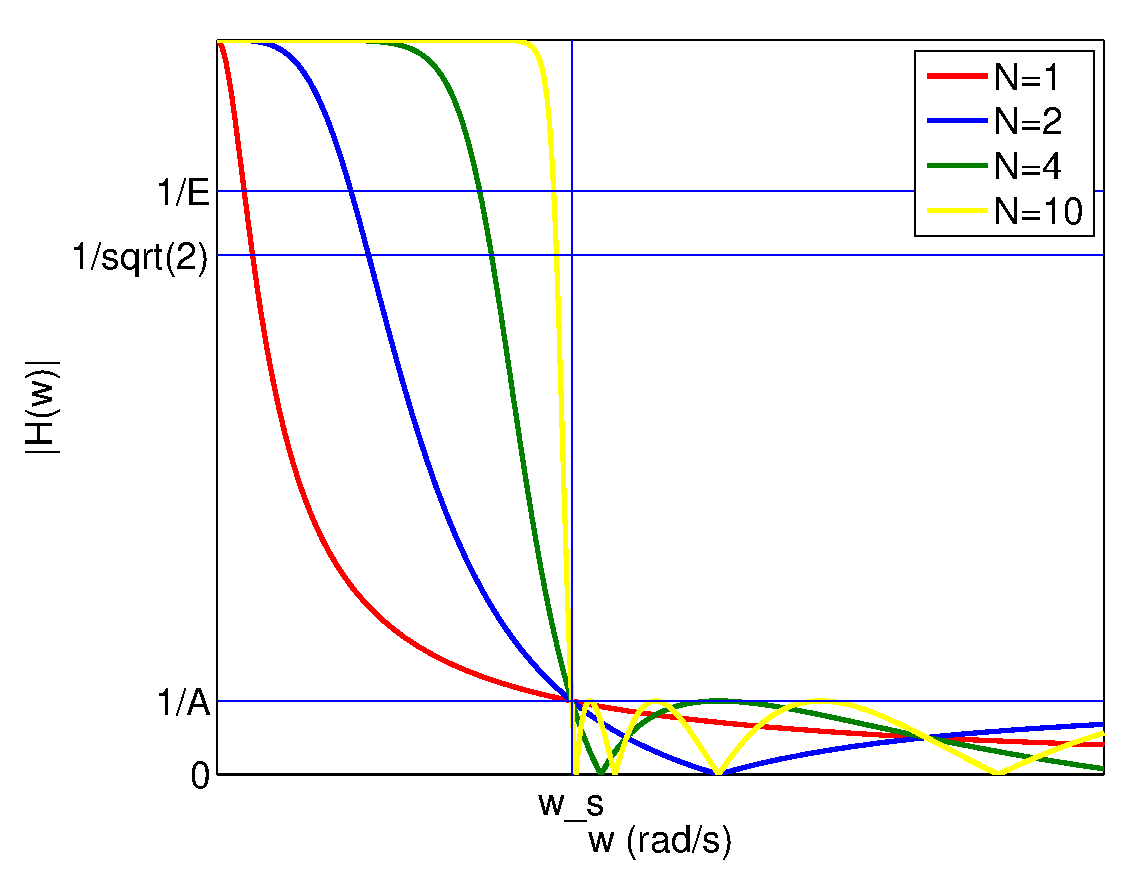
\includegraphics[width=3.5cm]{Figures/FiltroPB_Cheby2}
  }
  
  \visible<3->{
  \hspace{0.8cm}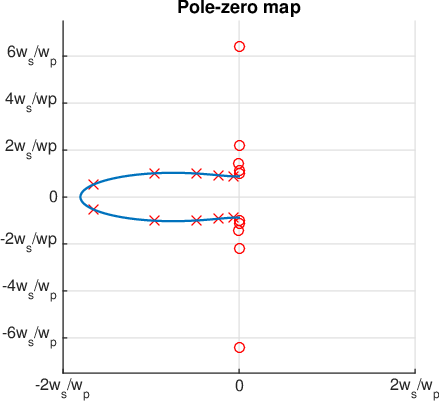
\includegraphics[width=2.2cm]{Figures/PolesCheby2.png}}
  
  \end{column}
  \end{columns}
  
  \footnotesize
  
  \vspace{0.1cm}
  
  
  
  
  
  \vspace{0.1cm}
  
  
  \footnotesize
  \begin{itemize}
  
  \visible<4->{
  
  \item Para una $\omega_s$ fija,
   si aumenta $N$ disminuye ancho de la banda de transición.
  
  
  }
  
  \visible<5->{
   \item Determinar el filtro de menor $N$ para valores dados de  $\omega_p$, $\omega_s$, $\alpha_p$, $\alpha_s$.
   }
   \vspace{0.1cm}
   {
  
   \color{gray}
  
   \scriptsize
  
   \vspace{-0.1cm}
  
   \visible<6->{
      $\!\!\!\!\left . \begin{array}{l}
    \alpha_p=-20 log_{10} \frac{1}{E} \\ \alpha_s=-20 log_{10} \frac{1}{A}\end{array}\right \}$ }   \visible<7->{ $\rightarrow \displaystyle\left . \begin{array}{l}
  E= 10^{\frac{ \alpha_p}{20}} \\ A=10^{\frac{ \alpha_s}{20}} \end{array}\right \}$ $\rightarrow \epsilon=\sqrt{E^2-1}$ }
  
  \vspace{-0.3cm}
  
   \visible<6->{
   $
   |H(j\omega_s)|^2=\frac{1}{1+\epsilon^2 \frac{cosh^2( N\cdot acosh(\omega_s/\omega_p))}{cos^2(N\cdot acos(1))}}=\frac{1}{A^2} \rightarrow$}   \visible<8->{\alert{$
  N=\frac{acosh \left ( \frac{\sqrt{A^2-1}}{\epsilon} \right)}{acosh(\omega_s/\omega_p)} $} $\rightarrow N=\frac{acosh \frac{1}{k_1}}{acosh\frac{1}{k}} $
    }
  
   }
  
  \end{itemize}
  \end{frame}


%%%%%%%%%%%%%%%%%%%%%%%%%%%%%%%

\begin{frame}\frametitle{Filtro de Chebyshev Tipo II (ejemplo)}
  
  \begin{itemize}{\scriptsize
    \item \color{olivegreen} Determinar el filtro de Chebyshev tipo II de orden más bajo con una atenuación en la banda de paso máxima de 1dB a 1KHz y una atenuación mínima en la banda de supresión de 40dB a 5KHz.
  
    \begin{columns}[T]
      \hspace{0.7cm}\begin{column}{7.1cm}
        \color{gray}
        
        \visible<1->{
        
        $\begin{array}{l}\!\!\!\left .\begin{array}{l}\omega_p=2\pi*1000\\
        \omega_s=2\pi*5000\\
        \alpha_p=1dB\\
        \alpha_s=40\end{array}\!\!\!\right \} \rightarrow\\ \: \\ \: \end{array}$ } $\!\!\!\!\!\!\begin{array}{l}E= 10^{\frac{ \alpha_p}{20}}=1.122 \\ A=10^{\frac{ \alpha_s}{20}}=100\\ \epsilon=\sqrt{E^2-1}=0.5088 \\
        N\!=\!\frac{acosh \!\left (\! \frac{\sqrt{A^2-1}}{\epsilon}\! \right)}{acosh(\omega_s/\omega_p)} \!=\!2.61 \rightarrow 3 \end{array}$
      \end{column}
      \hspace{-0.9cm}\begin{column}{4cm}
        \vspace{-0.2cm}
        \visible<2->{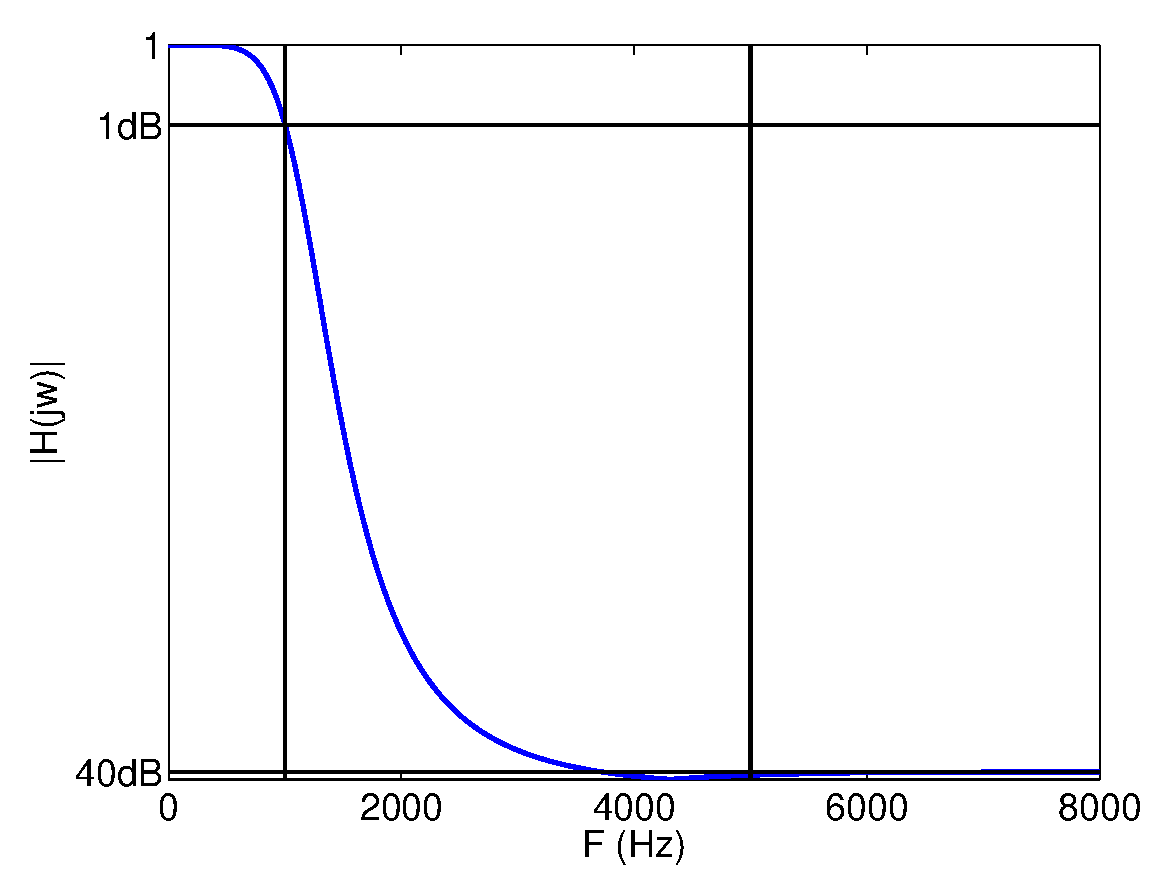
\includegraphics[width=4cm]{./Figures/FiltroPB_Cheby2Ex.eps}}
      \end{column}
    \end{columns}
  }
  \visible<3->{\vspace{-0.5cm}\footnotesize
  \item Con Matlab:
  
  \begin{itemize}
    \item \alert{\texttt{[N,wc]=cheb2ord(wp,ws,ap,as,'s')}}
    \begin{itemize}
      \color{gray}
      \item Calcula el orden \texttt{N} del filtro y la frecuencia de corte \texttt{wc}.
      \item \texttt{wp}, \texttt{ws} en rad/s.
      \item \texttt{ap}, \texttt{as} en dB.
      \item 's' para que calcule los valores del filtro de continuo.
    \end{itemize}
      \item \alert{\texttt{[B,A]=cheby2(N,as,wc,'low','s')}}
    \begin{itemize}
      \color{gray}
      \item Calcula el numerador \texttt{B} y denominador \texttt{A} de $H(s)$.
    \end{itemize}
    \item \alert{\texttt{[Hw,w]=freqs(B,A)}}
    \begin{itemize}
      \color{gray}
      \item Calcula la $H(j\omega)$ del filtro para las frecuencias \texttt{w}.
    \end{itemize}  
  \end{itemize}
  }
  \end{itemize}
  
\end{frame}
  
  
%%%%%%%%%%%%%%%%%%%%%%%%%%%%%%%%%%%%
  

  \begin{frame}
      \frametitle{Filtro Elíptico - I}
      
       \vspace{-0.2cm}
      
      \begin{columns}[T]
      \hspace{0.3cm}\begin{column}{7.5cm}
      
      \footnotesize
      
      
      \visible<1->{
      
      \hspace{0.3cm}\alert{$\displaystyle |H(jw)|^2\!=\!\frac{1}{1\!+\!\epsilon^2 R_N^2(w/\omega_p)}$}
      
      \vspace{0.1cm}
      
      \hspace{0.3cm}$R_N(w)=\frac{num(w)}{den(w)}$\hspace{1cm}$R_N(1/w)=1/R_N(w)$
      
      \vspace{0.1cm}
      
      \hspace{0.3cm}Raices $num(w)$  estan en $0<w<1$
      
      \vspace{0.1cm}
      
      \hspace{0.3cm}Raices $den(w)$ estan en $1<w<\infty$
      
      
      }
      
      \vspace{0.1cm}
      
      \hspace{0.3cm}\alert{$\displaystyle  H(s)=E_0\frac{ K(s) \prod_{l=1}^{floor(N/2)} (s^2+\omega_{zl}^2)}{\prod_{l=1}^{N} (s-p_l)}$}
      
      
      \vspace{0.2cm}
      
      \scriptsize
      
       \hspace{0.3cm}con  $p_l\!=\!(\sigma_l\!+\!j\omega_{pl})$, $K(s)\!=\!1$ si $N$ par, $K(s)\!=\!s$  si $N$ impar
      
      
      \footnotesize
      
      \begin{itemize}
      
      \visible<2->{
      
      \item Para una $\omega_p$ fija,
       si aumenta $N$ disminuye ancho de la banda de transición.
      
      
      }
      
      
      
      \visible<3->{
       \item Determinar el filtro de menor $N$ para valores dados de  $\omega_p$, $\omega_s$, $\alpha_p$, $\alpha_s$.
       }
      
      \end{itemize}
      
      
      \end{column}
      \hspace{-0.3cm}\begin{column}{4cm}
      \visible<1->{
      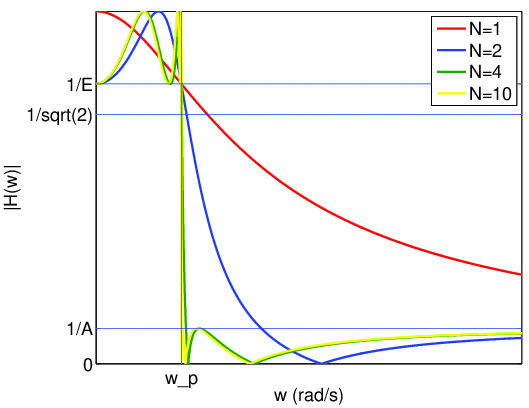
\includegraphics[width=3.5cm]{Figures/FiltroPB_Elip.png}
      }
      
      \visible<1->{
      \hspace{0.8cm}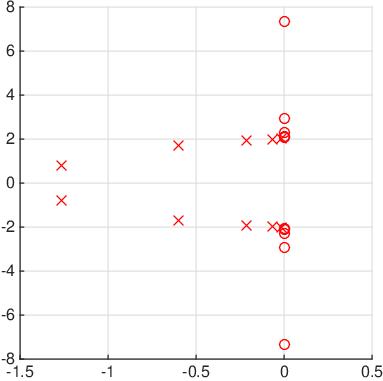
\includegraphics[width=2.5cm]{Figures/PolesEllip.png}
      }
      
      \end{column}
      \end{columns}
      
      \footnotesize
      
      \vspace{0.1cm}
      
      
      
      \footnotesize
      
      
       \vspace{0.1cm}
       {
      
       \color{gray}
      \visible<4->{
      \hspace{0.8cm}$\alpha_p=-20 log_{10} \frac{1}{E}$, \hspace{0.4cm}$\alpha_s=-20 log_{10}$,  \hspace{0.4cm}$k_1=\frac{\epsilon}{\sqrt{A^2-1}}$, \hspace{0.4cm}$ N= \frac{2log_{10}(4/k_1)}{log_{10}(1/\rho)}$
      
      \hspace{0.8cm}$\rho\!=\!\rho_0\!+\!2\rho_0^5\!+\!15\rho_0^9\!+\!150\rho_0^{13}$, \hspace{0.4cm}$\rho_0=\frac{1-\sqrt{k'}}{2(1+\sqrt{k'})}$, \hspace{0.4cm}$k'=\sqrt{1-k^2}$,\hspace{0.4cm}$k=\frac{\omega_p}{\omega_s}$
      
       \vspace{0.1cm}
      
      \hspace{0.8cm}Se necesita un computador para calcular los valores de $\omega_{zl}$, $\sigma_l$ y $\omega_{pl}$
      }
      
       }
      
\end{frame}

%%%%%%%%%%%%%%%%%%%%%%%%%%%%%%%

\begin{frame}
  \frametitle{Filtro Elíptico (ejemplo)}
  
  \vspace{-0.3cm}
  
  \begin{itemize}
  
  {
  \scriptsize
  \item \color{olivegreen} Determinar el filtro elíptico de orden más bajo con una atenuación en la banda de paso máxima de 1dB a 1KHz y una atenuación mínima en la banda de supresión de 40dB a 5KHz.
  
  \begin{columns}[T]
  \hspace{1cm}\begin{column}{7cm}
  \color{gray}
  
  \color{gray}
  $\!\!\!\!\!\!\begin{array}{ll}
  \omega_p\!=\!2\pi\!*\!1000 &
   \omega_s\!=\!2\pi\!*\!5000\\
   \alpha_p=1dB&
   \alpha_s=40\\
   E= 10^{\frac{ \alpha_p}{20}}=1.122  & A=10^{\frac{ \alpha_s}{20}}=100\\ \epsilon=\sqrt{E^2-1}=0.5088 &
   k_1=\frac{\epsilon}{\sqrt{A^2-1}}=0.0051\\
   k=\frac{\omega_s}{\omega_p}=\frac{1}{5}&
   k'=\sqrt{1-k^2}=0.9798\\
   \rho_0=\frac{1-\sqrt{k'}}{2(1+\sqrt{k'})}=0.00255 \end{array}$
  
  
  $\!\!\!\rho\!=\!\rho_0\!+\!2\rho_0^5\!+\!15\rho_0^9\!+\!150\rho_0^{13}\!=\!0.002551$
  
  \vspace{0.1cm}
  
  $\!\!\!N= \frac{2log_{10}(4/k_1)}{log_{10}(1/\rho)}=2.23  \rightarrow 3$
  
   \end{column}
  \hspace{-1cm} \begin{column}{4cm}
  
   \visible<2->{ 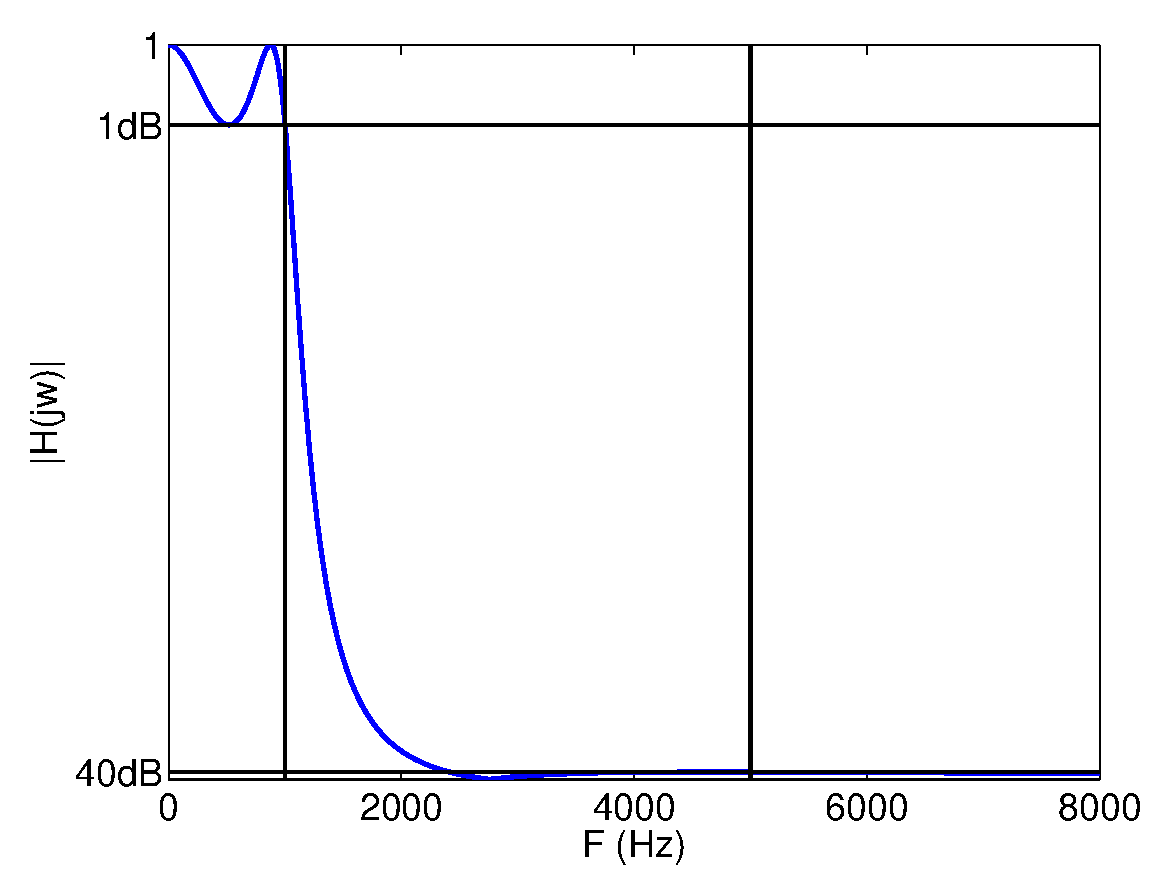
\includegraphics[width=4cm]{./Figures/FiltroPB_EllipEx.eps}}
  
   \end{column}
   \end{columns}
  
  }
  \visible<3->{
  {
  
  \vspace{0.1cm}
  
  \footnotesize
  \item Con Matlab:
  
  \vspace{-0.1cm}
  
  \begin{itemize}
  \item \alert{\texttt{[N,wp]=ellipord(wp,ws,ap,as,'s')}}
  \begin{itemize}
  \color{gray}
  \item Calcula el orden del filtro $N$ y la $\omega_p$.
  \item \texttt{wp}, \texttt{ws} en rad/s.
  \item \texttt{ap}, \texttt{as} en dB.
  \item 's' para que calcule los valores del filtro de continuo.
  \end{itemize}
  \item \alert{\texttt{[B,A]=ellip(N,as,ap,wp,'low','s')}}
  \begin{itemize}
  \color{gray}
  \item Calcula el numerador \texttt{B} y denominador \texttt{A} de $H(s)$.
  \end{itemize}
  \end{itemize}
  }
  }
  \end{itemize}
  
\end{frame}

\begin{frame}\frametitle{Resumen de filtro paso bajo: ordenes de Matlab}

  \begin{itemize}
    \item Cálculo del orden y frecuencia característica del filtro:
    \begin{itemize}
      \item \alert{\texttt{[N,wc]=buttord(wp,ws,ap,as,'s')}}
      \item \alert{\texttt{[N,wc]=cheb1ord(wp,ws,ap,as,'s')}}
      \item \alert{\texttt{[N,wc]=cheb2ord(wp,ws,ap,as,'s')}}
      \item \alert{\texttt{[N,wc]=ellipord(wp,ws,ap,as,'s')}}
    \end{itemize}
      \item Cálculo de la función de transferencia del filtro, $H(s)$:
    \begin{itemize}
      \item \alert{\texttt{[B,A]=butter(N,wc,'low','s')}}
      \item \alert{\texttt{[B,A]=cheby1(N,ap,wc,'low','s')}}
      \item \alert{\texttt{[B,A]=cheby2(N,ap,wc,'low','s')}}
      \item \alert{\texttt{[B,A]=ellip(N,ap,as,wc,'low','s')}}
    \end{itemize}
      \item Cálculo y representación del espectro del filtro, $H(j\omega)$.
    \begin{itemize}
      \item \alert{\texttt{[Hw,w]=freqs(B,A)}}
      \item \alert{\texttt{plot(w,abs(Hw))}}
      \item \alert{\texttt{plot(w,angle(Hw))}}
      \item \alert{\texttt{plot(w,unwrap(angle(Hw)))}}
    \end{itemize}
  \end{itemize}

\end{frame}


%%%%%%%%%%%%%%%%%%%%%%%%%%%%%%%%%%%%%%%%


\subsection{Filtro paso alta, paso banda y supresores de banda}

% \begin{frame}
% \frametitle{Filtro paso alta, paso banda y supresores de banda I}

% \footnotesize
% \begin{itemize}
% \item Las funciones de transferencia $H(\hat s)$ de los filtros  paso alta, paso banda y supresores de banda se pueden obtener a partir de la función de transferencia de un filtro paso baja $H_{LP}(s)$ a través de una transformación espectral $s=F(\hat s)$.
% \begin{itemize}
% \footnotesize
% \visible<2->{
% \item Filtro paso alta: \hspace{1.3cm}$s=\frac{\omega_p \hat \omega_p}{\hat s}$ \hspace{1.5cm} $- w \hat w=\omega_p \hat \omega_p$}
% \visible<3->{
% \item Filtro paso banda: \hspace{1.0cm} $s=\omega_p\frac{\hat s^2+\hat \omega_0^2}{\hat s (\hat \omega_{p2}-\hat \omega_{p1})}$
% \hspace{0.5cm}$w=\omega_p\frac{\hat w^2-\hat \omega_0^2}{\hat w (\hat \omega_{p2}-\hat \omega_{p1})}$

% \hspace{3.7cm}$\hat \omega_0^2=\hat \omega_{p1}\hat \omega_{p2}=\hat \omega_{s1}\hat \omega_{s2}$}

% \visible<4->{

% \item Filtro supresor de banda : $s=\omega_s\frac{\hat s (\hat \omega_{s2}-\hat \omega_{s1})}{\hat s^2+\hat \omega_0^2}$ \hspace{0.5cm}$w=\omega_s\frac{\hat w (\hat \omega_{s2}-\hat \omega_{s1})}{\hat \omega_0^2-\hat w^2}$

% \hspace{3.7cm}$\hat \omega_0^2=\hat \omega_{p1}\hat \omega_{p2}=\hat \omega_{s1}\hat \omega_{s2}$

% }

% \end{itemize}

% \visible<5->{
% \item Se cogen las especificaciones del filtro en que hay que hacer, y se calculan las correspondientes al filtro paso baja con las fórmulas de la frecuencia (suponiendo que $\omega_p=1$). }
% \visible<6->{
% \item Acto seguido se calcula la función de transferencia del filtro paso baja asociado al filtro paso baja.}
% \visible<7->{
% \item La función de transferencia del filtro destino será $H(\hat s)=H_{LP}(s=F(\hat s))$ con la $F(\hat s)$ del filtro correspondiente  correspondiente}
% \end{itemize}

% \end{frame}

% %%%%%%%%%%%%%%%%%%%%%%%%%%%%%%%
% % Transformaciones Espectrales
% %%%%%%%%%%%%%%%%%%%%%%%%%%%%%%%
  

% \begin{frame}{Transformaciones espectrales}
%   \begin{columns}
%       \begin{column}{0.45\textwidth}
%           \centering\small
%           Paso bajo $\rightarrow$ Paso alto\\
%           \[s=\frac{\omega_p\hat{\omega}_p}{\hat{s}}\Leftrightarrow\omega=\frac{-\omega_p\hat{\omega}_p}{\hat{\omega}}\]
%       \end{column}
%       \begin{column}{0.55\textwidth}
%           \centering
%           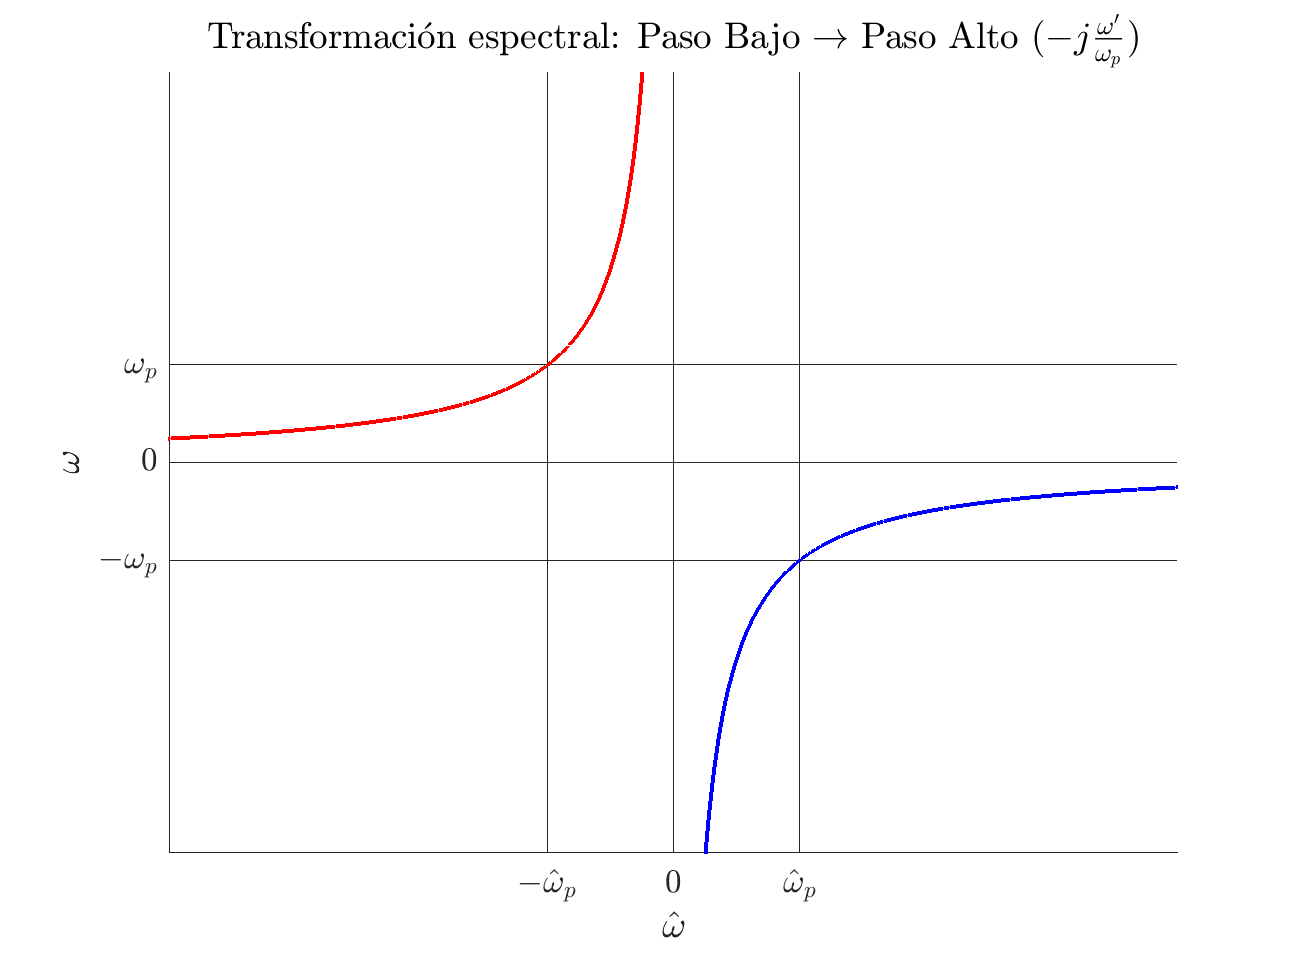
\includegraphics[height=4cm]{Figures/TE_1a.png}\\
%       \end{column}
%   \end{columns}
%   \begin{center}
%       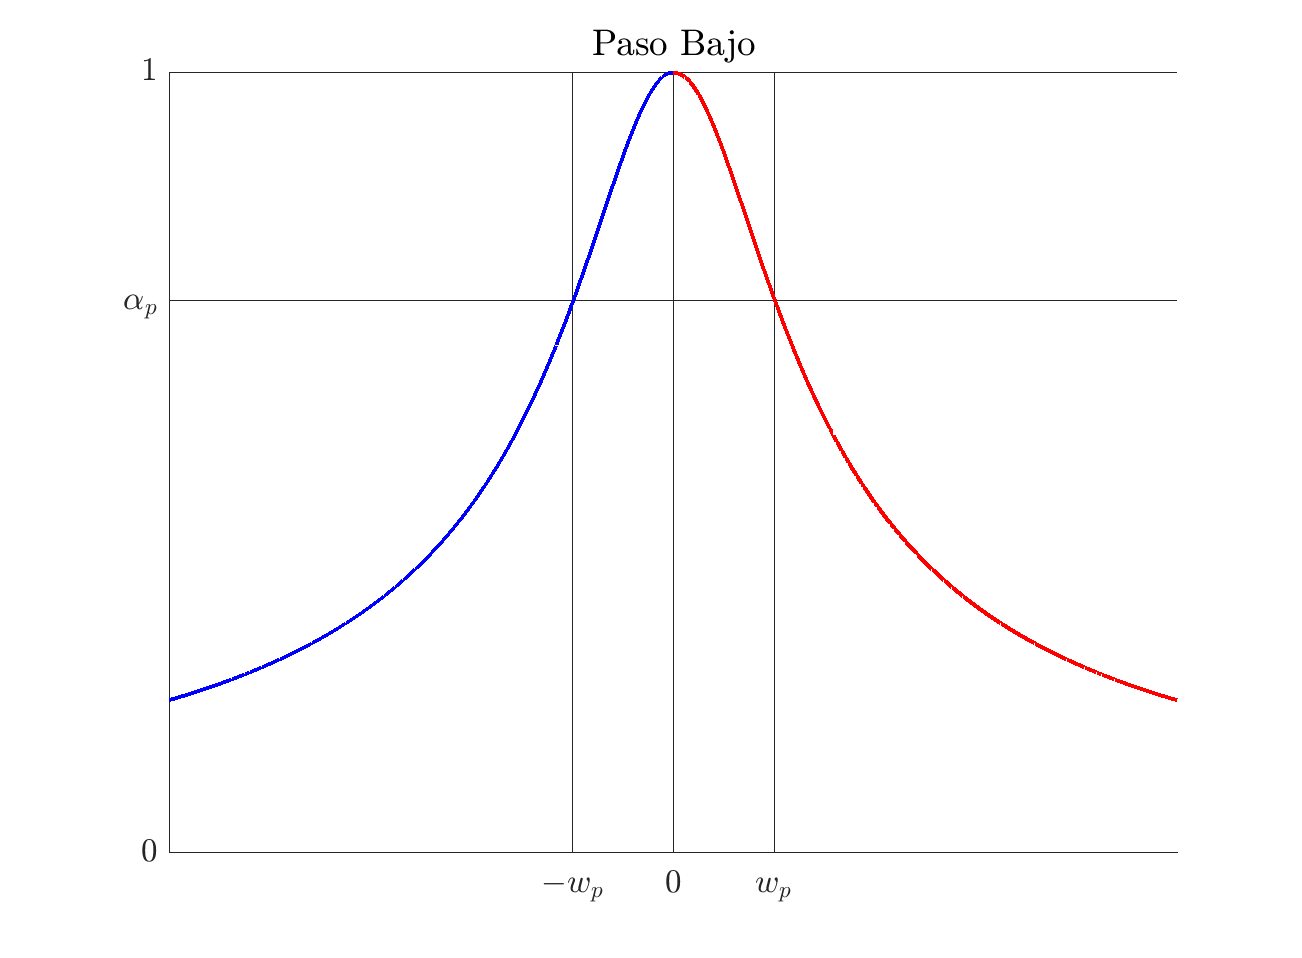
\includegraphics[height=4.25cm]{Figures/TE_1b.png}%
%       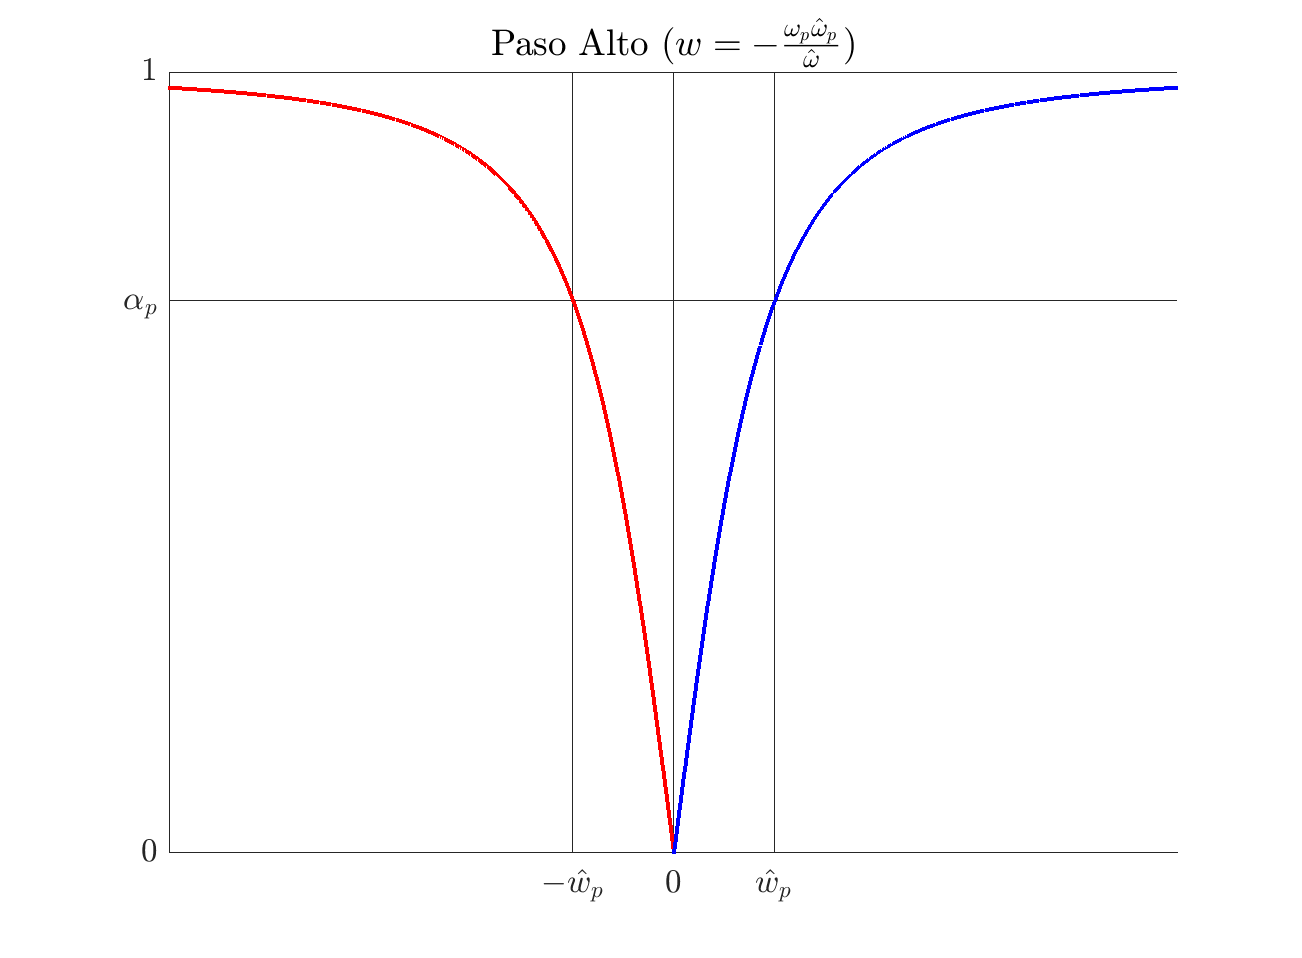
\includegraphics[height=4.25cm]{Figures/TE_1c.png}
%   \end{center}
% \end{frame}

% \begin{frame}{Transformaciones espectrales}
% \begin{columns}
%   \begin{column}{0.45\textwidth}
%       \centering\footnotesize
%       Paso bajo $\rightarrow$ Paso banda\\
%       \[s=\frac{\omega_p(\hat{s}^2+\hat{\omega_0}^2)}{\hat{s}(\hat{\omega}_{p_2}-\hat{\omega}_{p_1})} \Leftrightarrow
%       \omega=\frac{\omega_p(\hat{\omega}^2-\hat{\omega}_0^2)}{\hat{\omega}(\hat{\omega}_{p_2}-\hat{\omega}_{p_1})}\]\\
%   \end{column}
%   \begin{column}{0.55\textwidth}
%       \centering
%       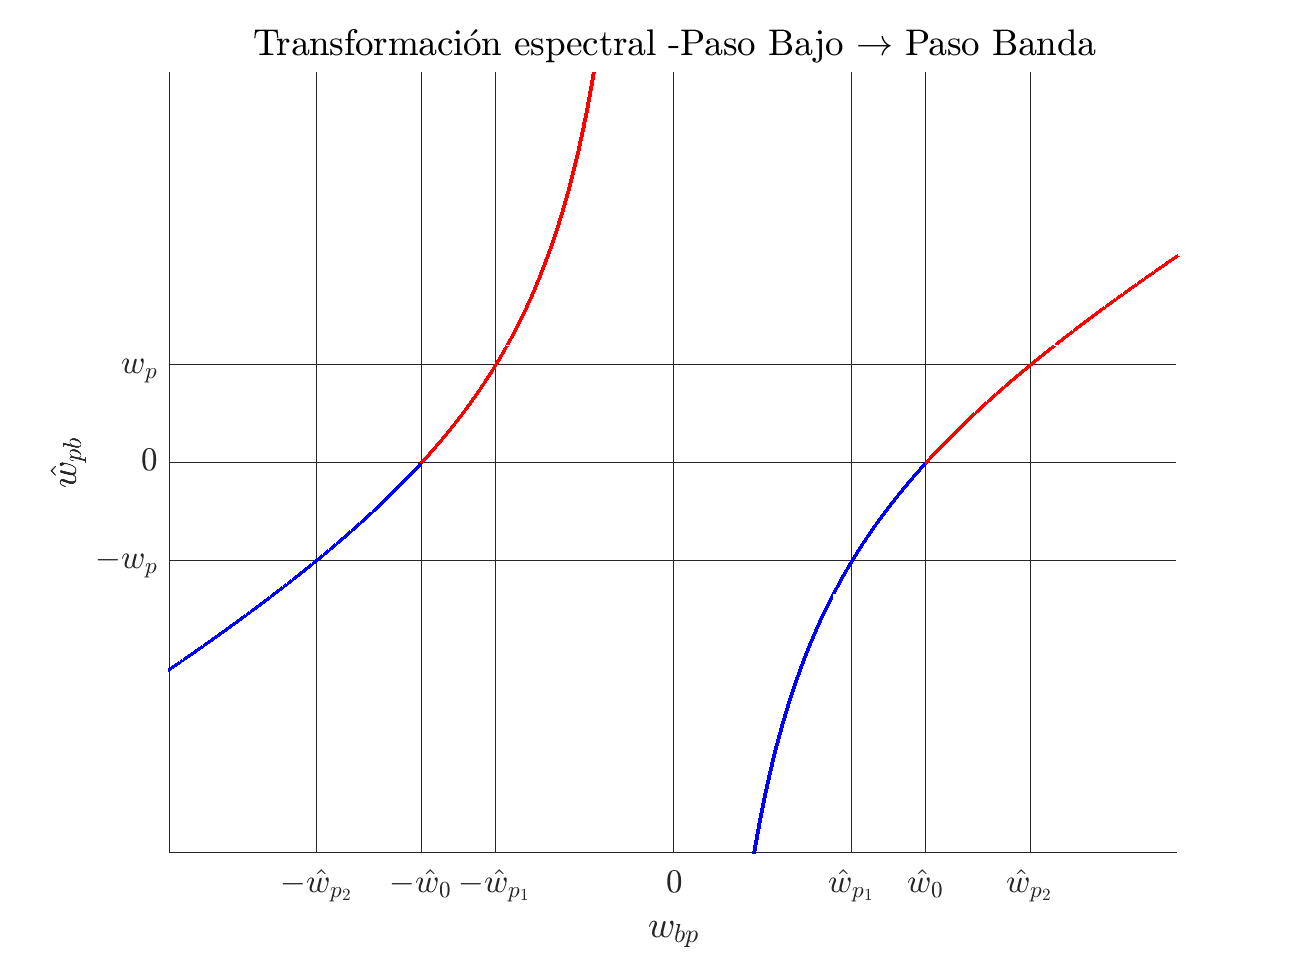
\includegraphics[height=4cm]{Figures/TE_2a.png}\\
%   \end{column}
% \end{columns}
% \begin{center}
%   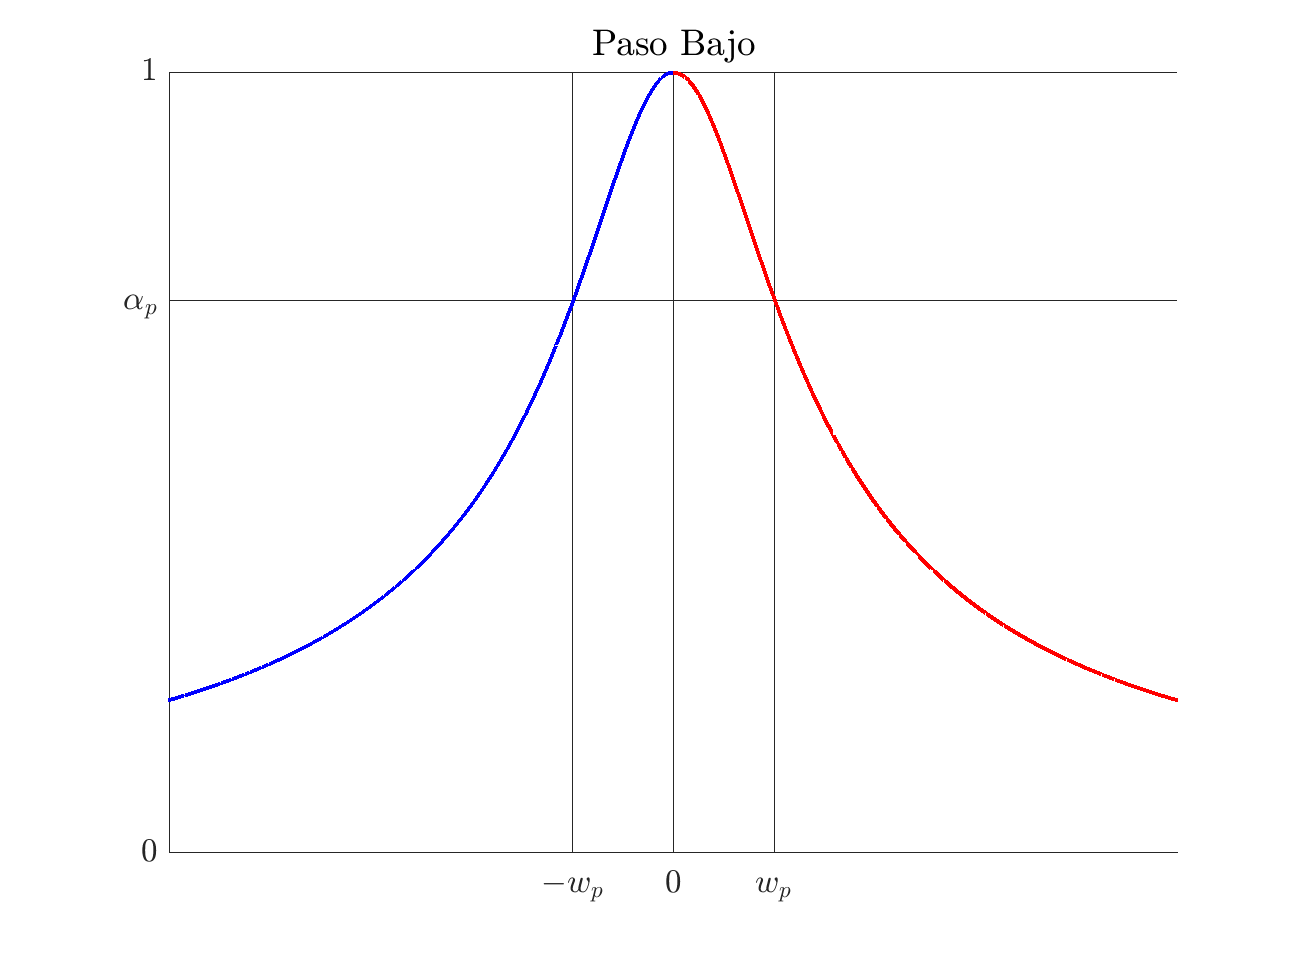
\includegraphics[height=4.25cm]{Figures/TE_2b.png}%
%   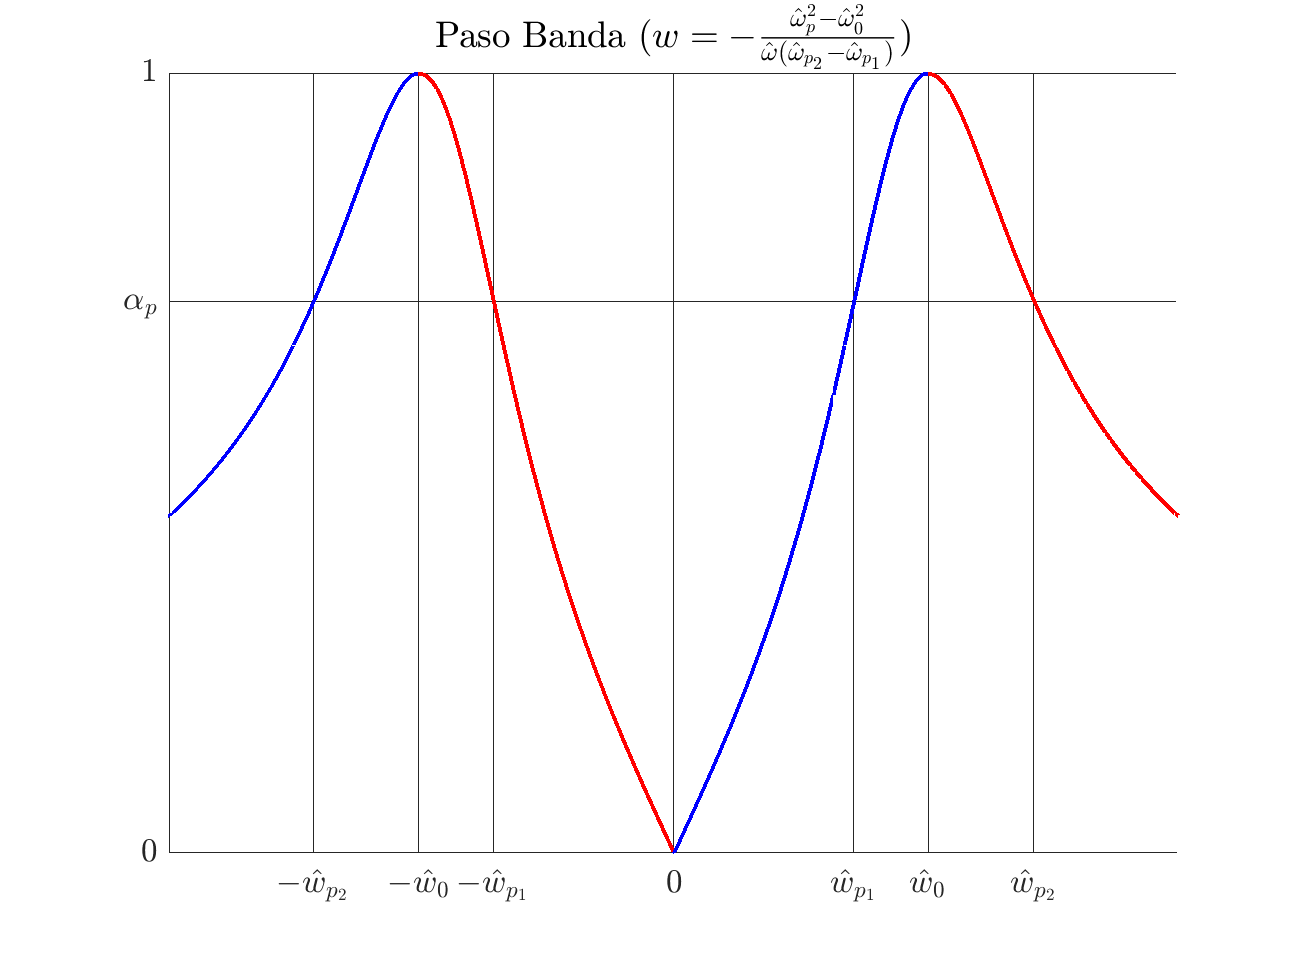
\includegraphics[height=4.25cm]{Figures/TE_2c.png}
% \end{center}
% \end{frame}

% \begin{frame}{Transformaciones espectrales}
% \begin{columns}
%   \begin{column}{0.45\textwidth}
%       \centering\footnotesize
%       Paso bajo $\rightarrow$ Supresor de banda\\
%       \[s=\omega_s\frac{\hat{s}(\hat{\omega}_{s_2}-\hat{\omega}_{s_1})}{\hat{s}^2+\hat{\omega_0}^2}\Leftrightarrow\omega=\omega_s\frac{\hat{\omega}(\hat{\omega}_{s_2}-\hat{\omega}_{s_1})}{\hat{\omega_0}^2-\hat{\omega}^2}\]\\
%   \end{column}
%   \begin{column}{0.55\textwidth}
%       \centering
%       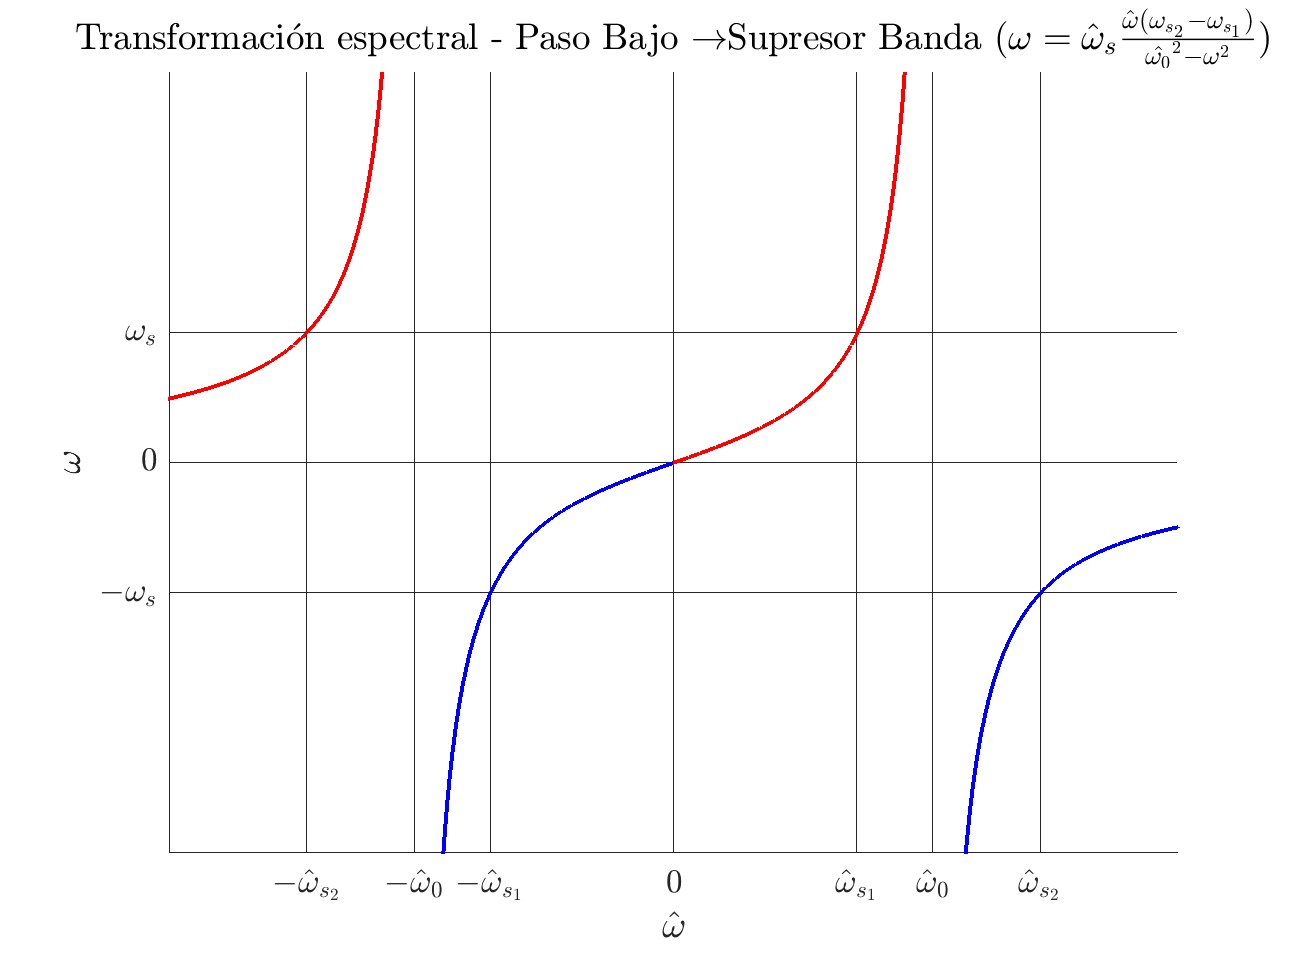
\includegraphics[height=4cm]{Figures/TE_3a.png}\\
%   \end{column}
% \end{columns}
% \begin{center}
%   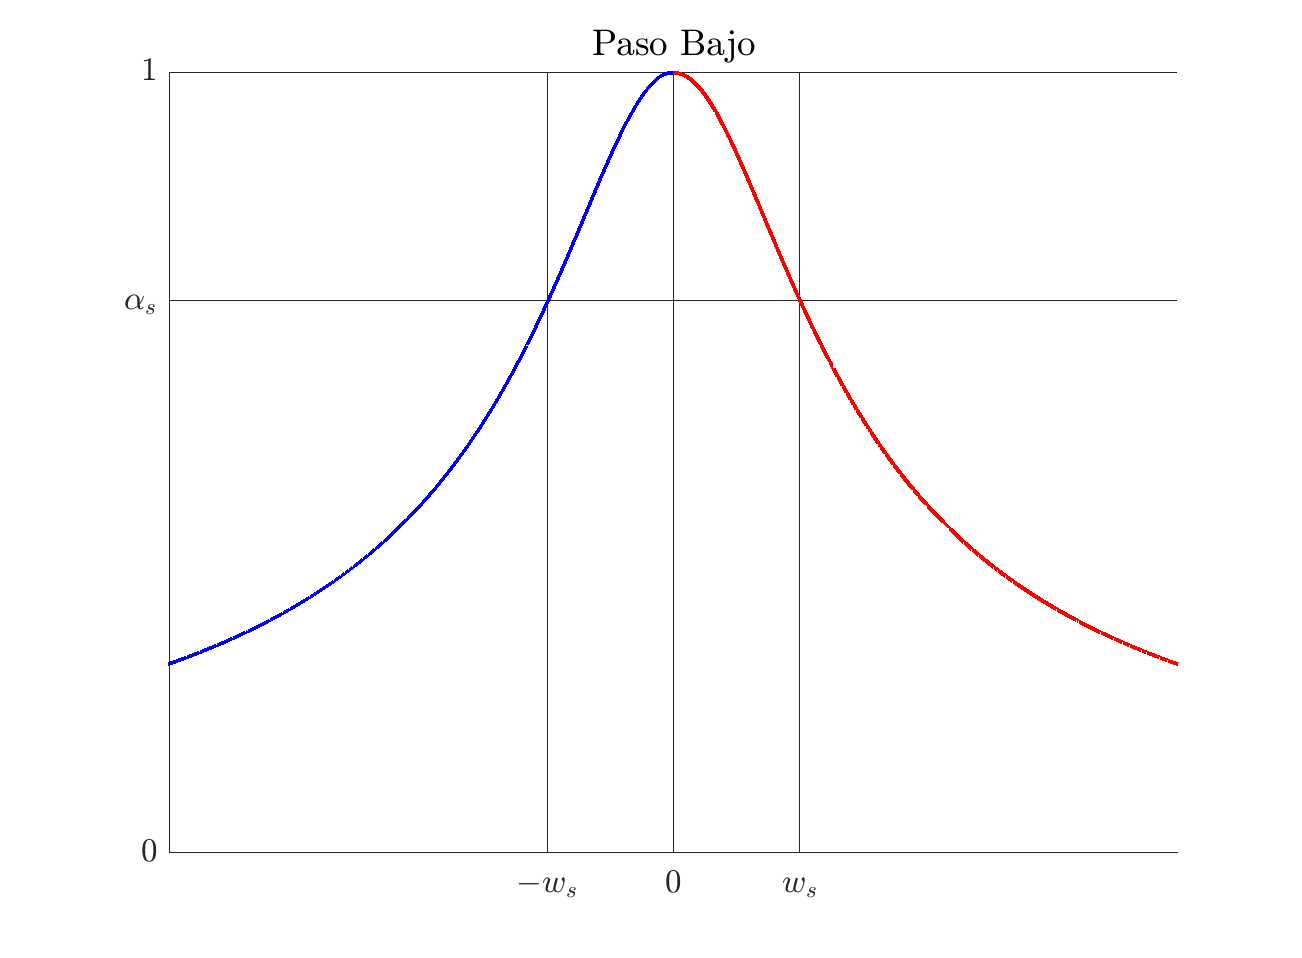
\includegraphics[height=4.25cm]{Figures/TE_3b.png}%
%   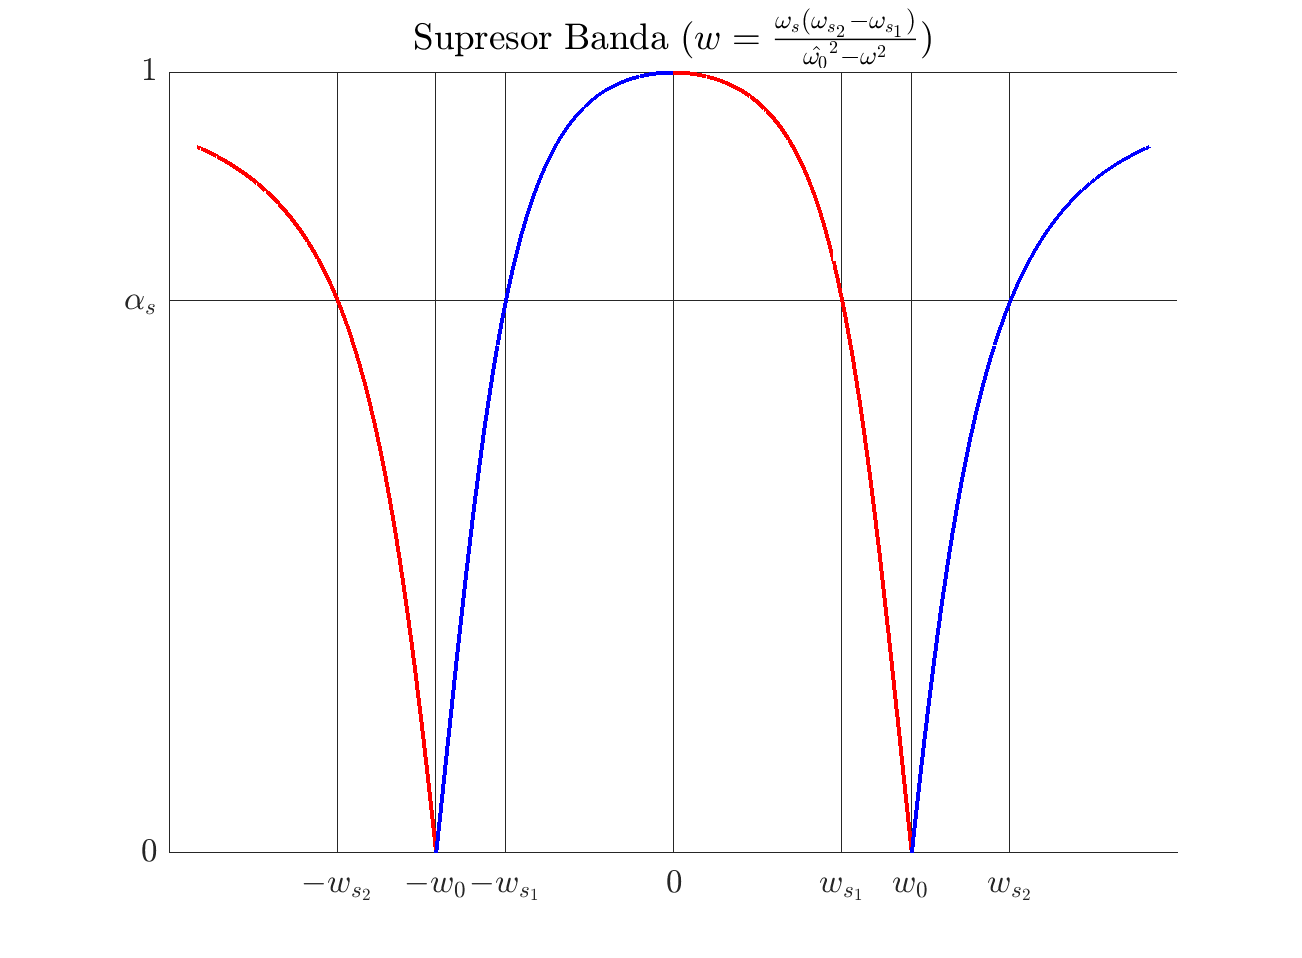
\includegraphics[height=4.25cm]{Figures/TE_3c.png}
% \end{center}
% \end{frame}

%%%%%%%%%%%%%%%%%%%%%%%%%%%%%%%%%%%%%%%%%%%
% \subsection{Filtro paso alta, paso banda y supresores de banda}

\begin{frame}
\frametitle{Filtro paso alta, paso banda y supresores de banda I}

  \footnotesize
  \begin{itemize}
  \item Las funciones de transferencia $H(\hat s)$ de los filtros  paso alta, paso banda y supresores de banda se pueden obtener a partir de la función de transferencia de un filtro paso baja $H_{LP}(s)$ a través de una transformación espectral $s=F(\hat s)$.
  \begin{itemize}
    \footnotesize
    \item Filtro paso alta: \hspace{1.3cm}$s=\frac{\omega_p \hat \omega_p}{\hat s}$ \hspace{1.5cm} $-\omega \hat \omega=\omega_p \hat \omega_p$
    \item Filtro paso banda: \hspace{1.0cm} $s=\omega_p\frac{\hat s^2+\hat \omega_0^2}{\hat s (\hat \omega_{p2}-\hat \omega_{p1})}$
    \hspace{0.5cm}$\omega=\omega_p\frac{\hat\omega^2-\hat \omega_0^2}{\hat \omega (\hat \omega_{p2}-\hat \omega_{p1})}$

    \hspace{3.7cm}$\hat \omega_0^2=\hat \omega_{p1}\hat \omega_{p2}=\hat \omega_{s1}\hat \omega_{s2}$
    \item Filtro supresor de banda : $s=\omega_s\frac{\hat s (\hat \omega_{s2}-\hat \omega_{s1})}{\hat s^2+\hat \omega_0^2}$ \hspace{0.5cm}$\omega=\omega_s\frac{\hat \omega (\hat \omega_{s2}-\hat \omega_{s1})}{\hat \omega_0^2-\hat \omega^2}$

    \hspace{3.7cm}$\hat \omega_0^2=\hat \omega_{p1}\hat \omega_{p2}=\hat \omega_{s1}\hat \omega_{s2}$
  \end{itemize}

\item Pasar especificaciones del filtro deseado a paso bajo (suponiendo $\omega_p=1$).
\item Calcula la función de transferencia del filtro paso baja asociado al filtro paso baja.
\item La función de transferencia del filtro destino será $H(\hat s)=H_{LP}(s=F(\hat s))$ con la $F(\hat s)$ del filtro correspondiente
\end{itemize}

\end{frame}

\begin{frame}{Transformaciones espectrales}
  \begin{columns}
      \begin{column}{0.45\textwidth}
          \centering\small
          Paso bajo $\rightarrow$ Paso alto\\
          \[s=\frac{\omega_p\hat{\omega}_p}{\hat{s}}\Leftrightarrow\omega=\frac{-\omega_p\hat{\omega}_p}{\hat{\omega}}\]
      \end{column}
      \begin{column}{0.55\textwidth}
          \centering
          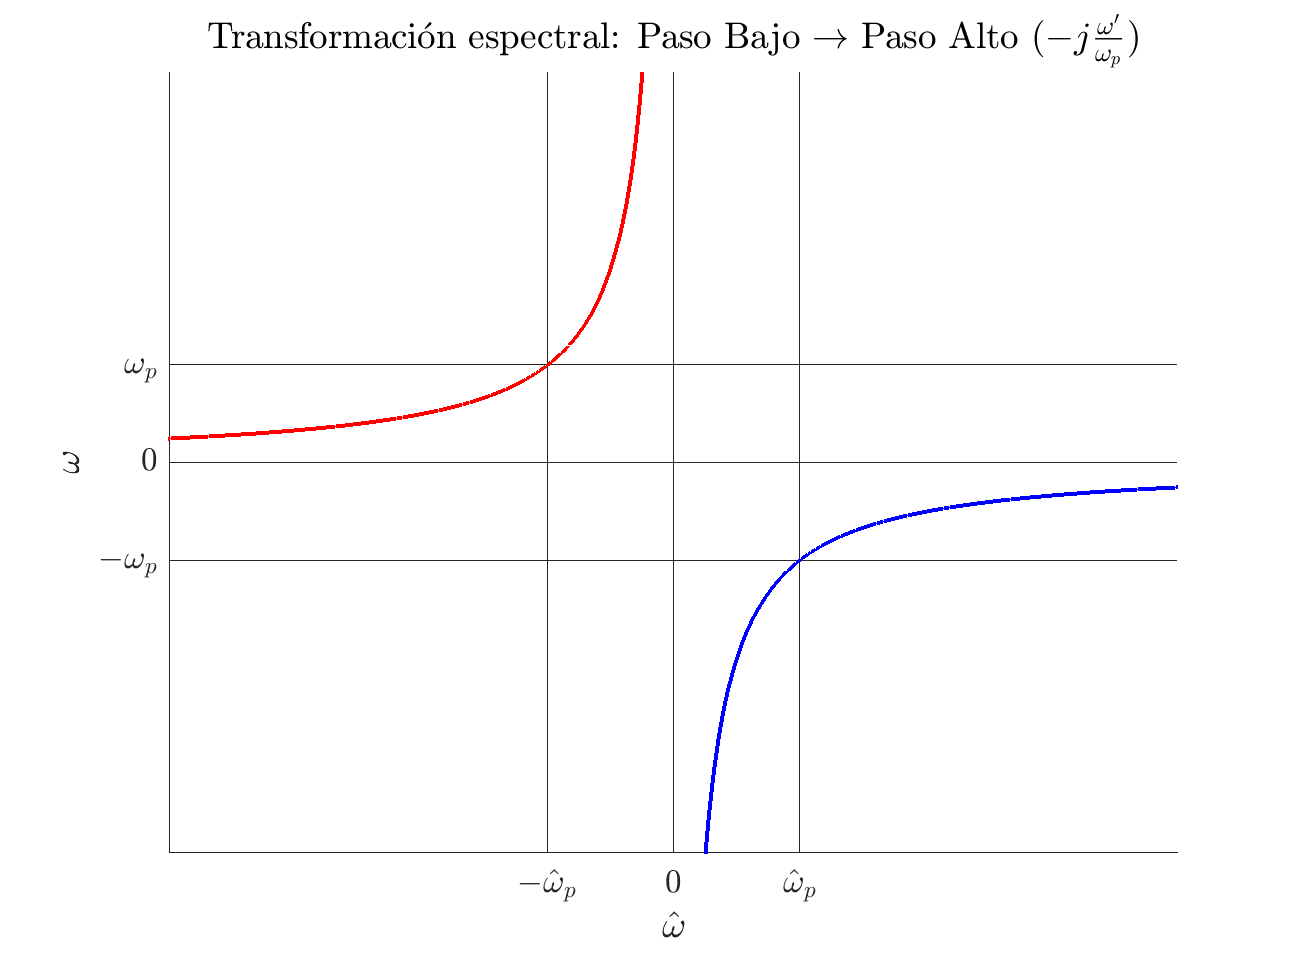
\includegraphics[height=4cm]{Figures/TE_1a.png}\\
      \end{column}
  \end{columns}
  \begin{center}
      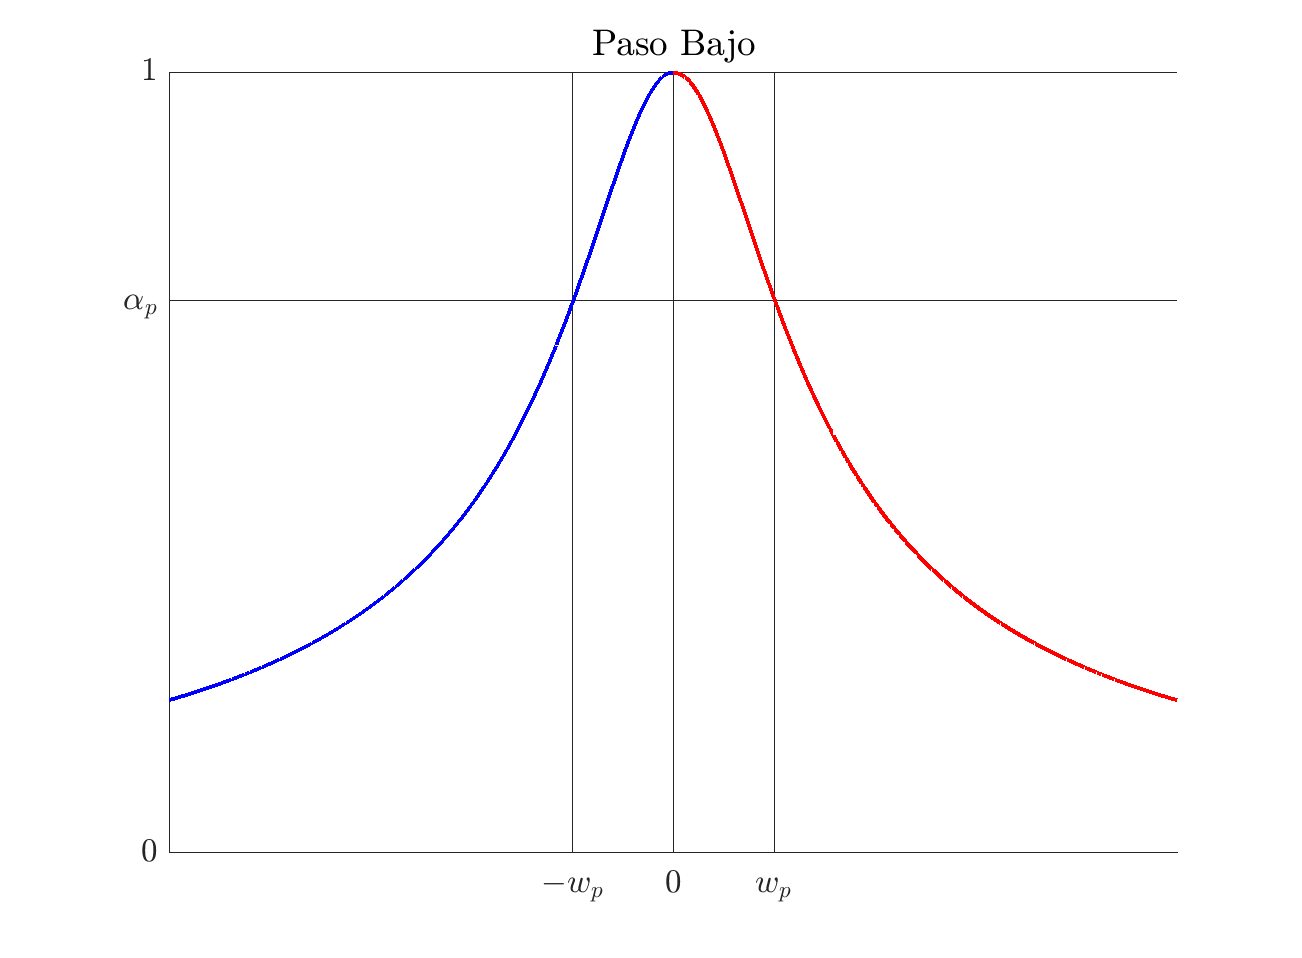
\includegraphics[height=4.25cm]{Figures/TE_1b.png}%
      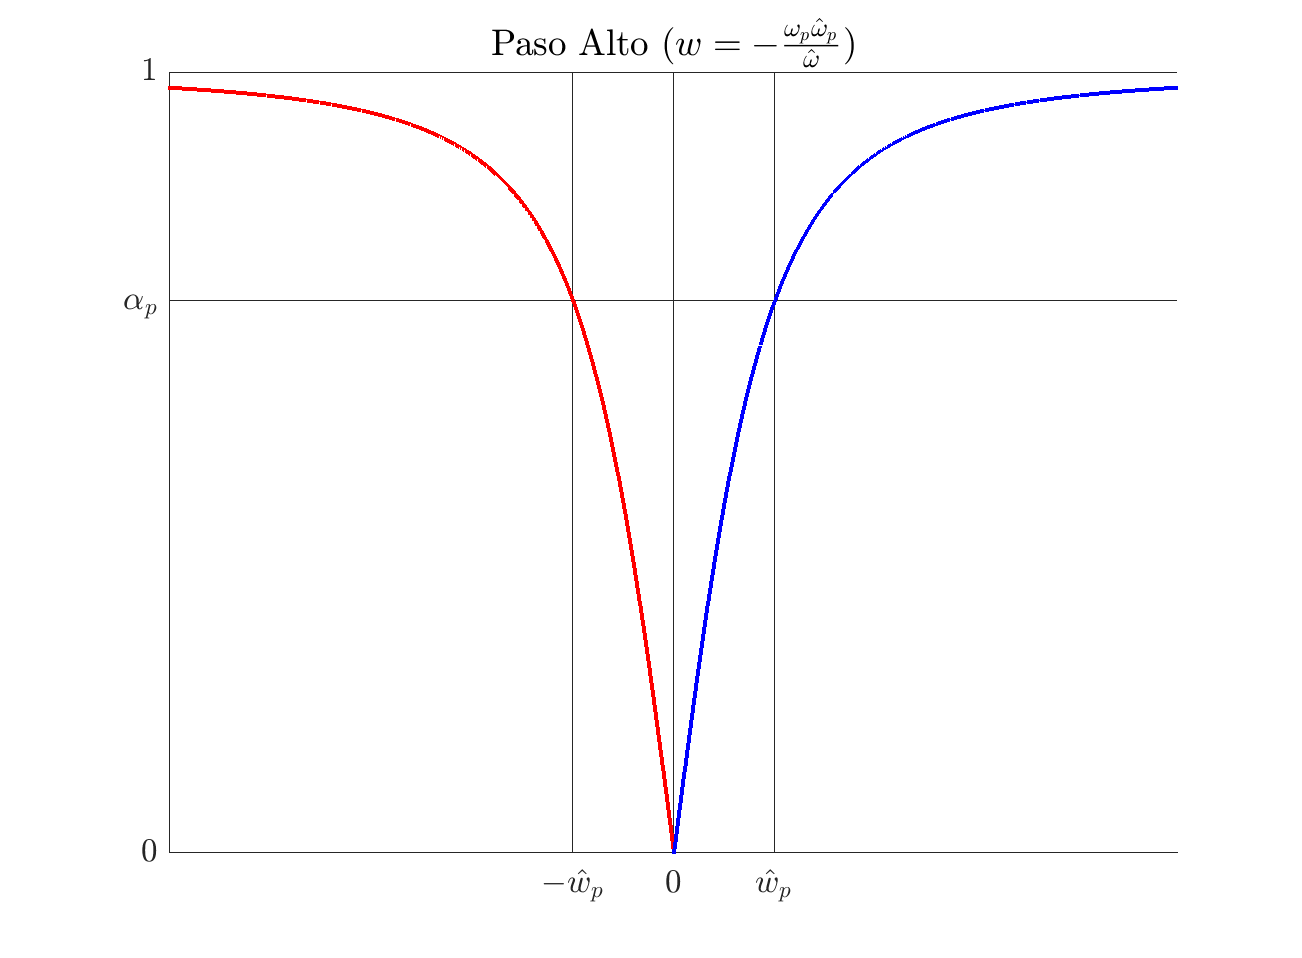
\includegraphics[height=4.25cm]{Figures/TE_1c.png}
  \end{center}
\end{frame}

\begin{frame}{Transformaciones espectrales}
\begin{columns}
  \begin{column}{0.45\textwidth}
      \centering\footnotesize
      Paso bajo $\rightarrow$ Paso banda\\
      \[s=\frac{\omega_p(\hat{s}^2+\hat{\omega_0}^2)}{\hat{s}(\hat{\omega}_{p_2}-\hat{\omega}_{p_1})} \Leftrightarrow
      \omega=\frac{\omega_p(\hat{\omega}^2-\hat{\omega}_0^2)}{\hat{\omega}(\hat{\omega}_{p_2}-\hat{\omega}_{p_1})}\]\\
  \end{column}
  \begin{column}{0.55\textwidth}
      \centering
      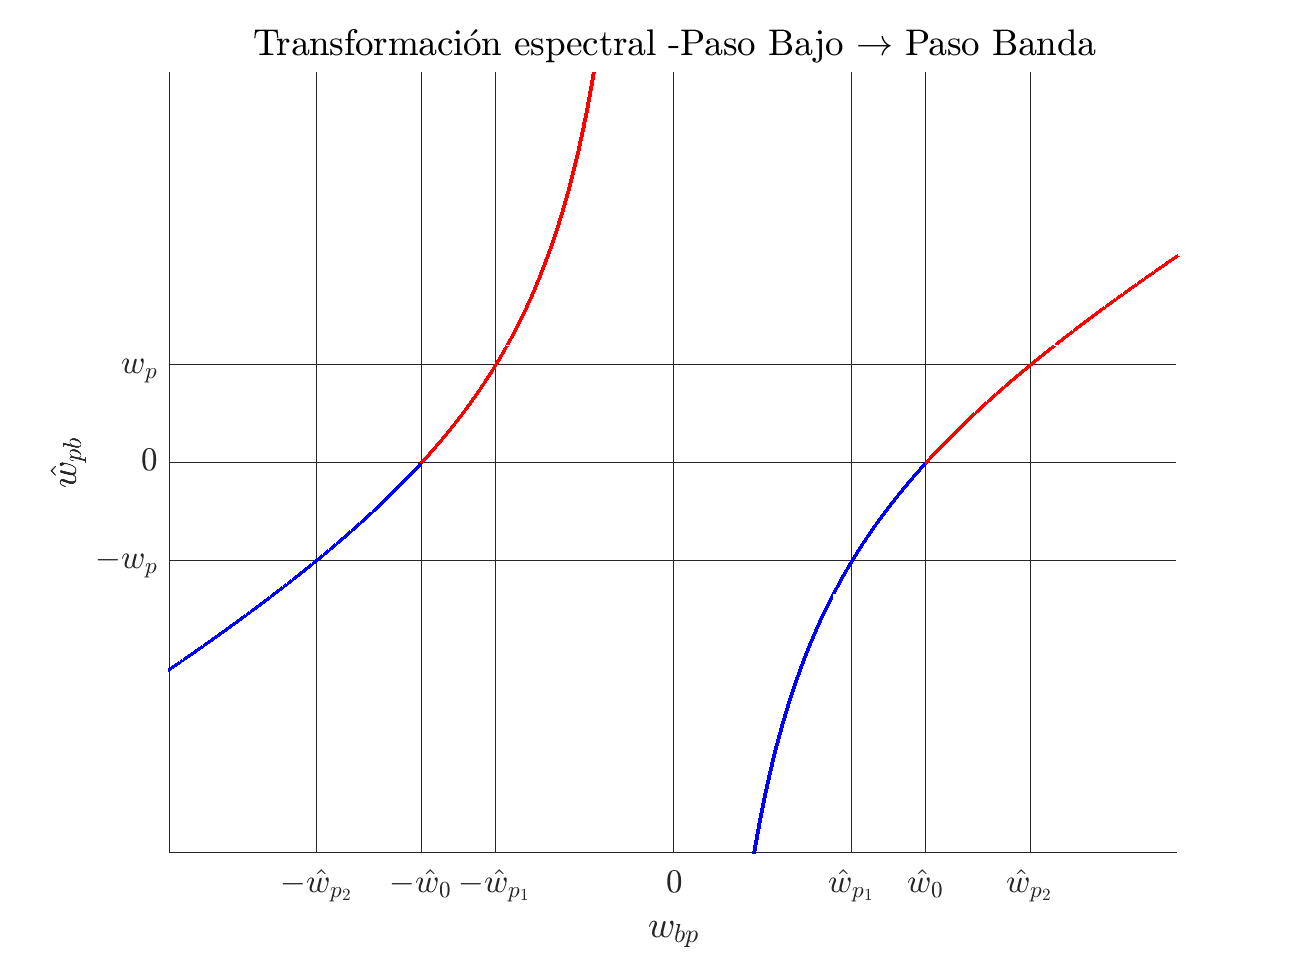
\includegraphics[height=4cm]{Figures/TE_2a.png}\\
  \end{column}
\end{columns}
\begin{center}
  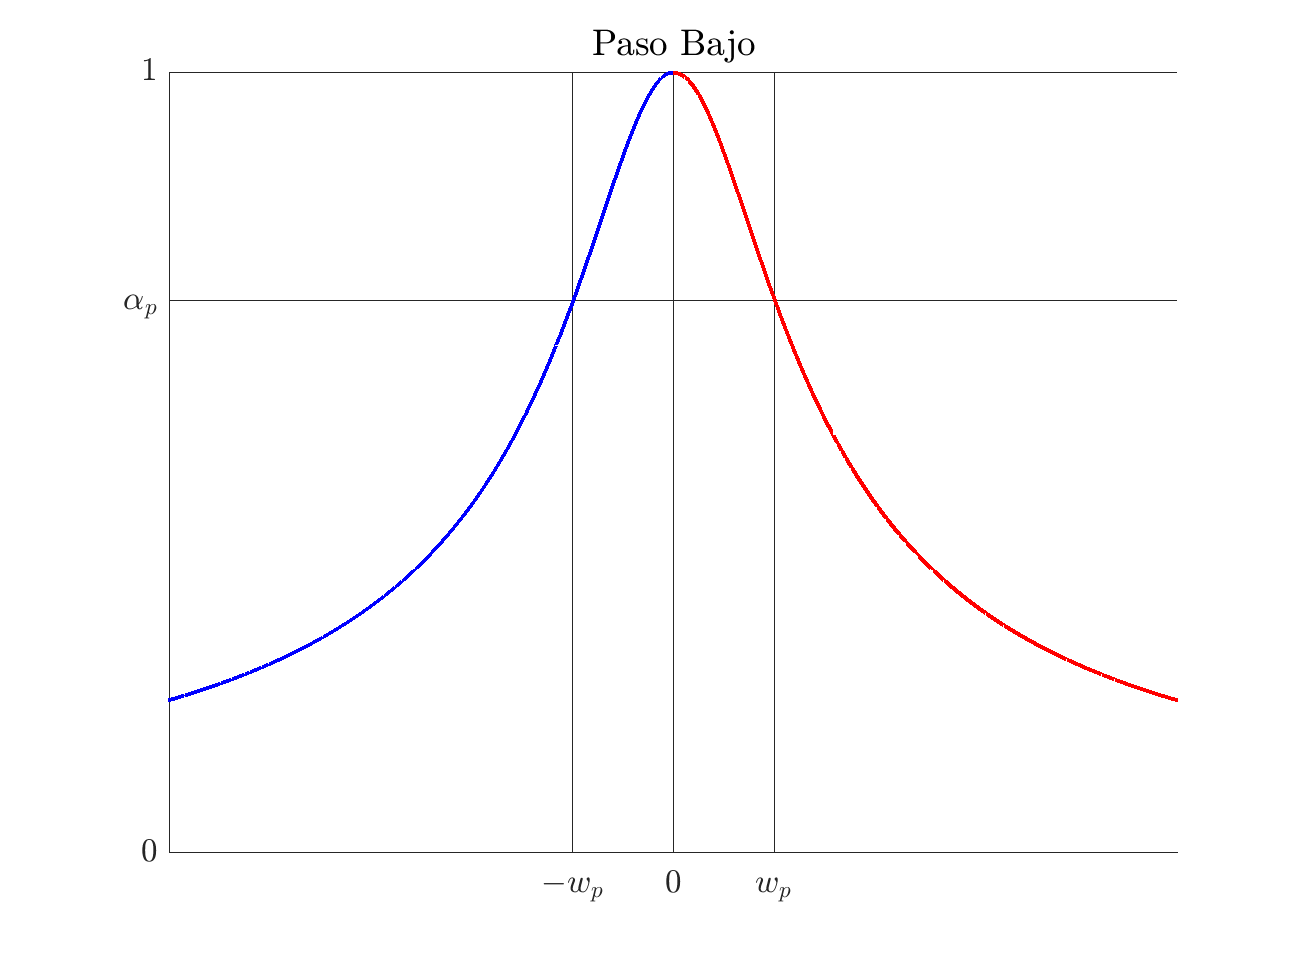
\includegraphics[height=4.25cm]{Figures/TE_2b.png}%
  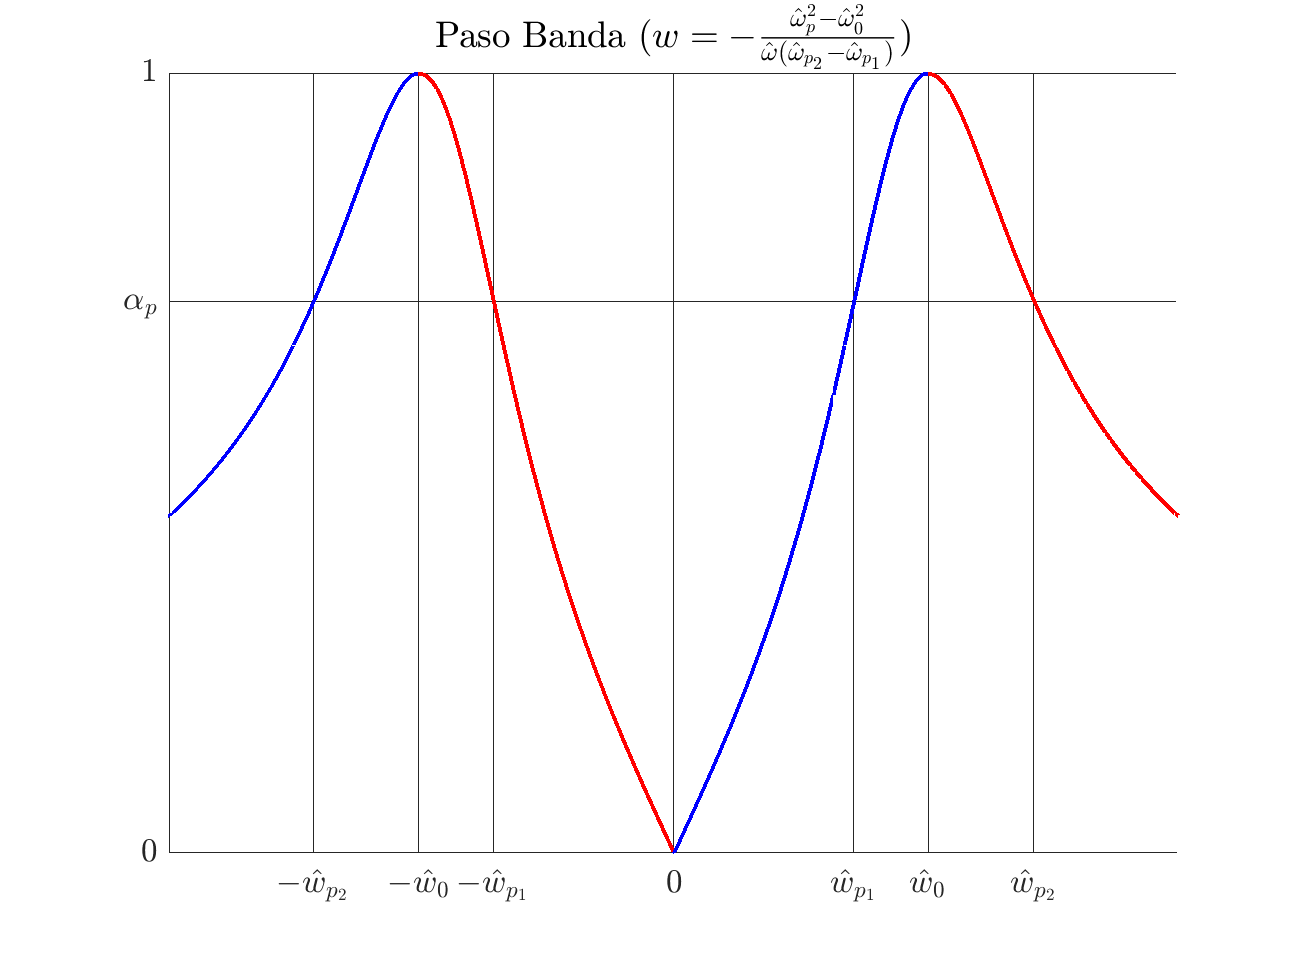
\includegraphics[height=4.25cm]{Figures/TE_2c.png}
\end{center}
\end{frame}


\begin{frame}{Transformaciones espectrales}
\begin{columns}
  \begin{column}{0.45\textwidth}
      \centering\footnotesize
      Paso bajo $\rightarrow$ Supresor de banda\\
      \[s=\omega_s\frac{\hat{s}(\hat{\omega}_{s_2}-\hat{\omega}_{s_1})}{\hat{s}^2+\hat{\omega_0}^2}\Leftrightarrow\omega=\omega_s\frac{\hat{\omega}(\hat{\omega}_{s_2}-\hat{\omega}_{s_1})}{\hat{\omega_0}^2-\hat{\omega}^2}\]\\
  \end{column}
  \begin{column}{0.55\textwidth}
      \centering
      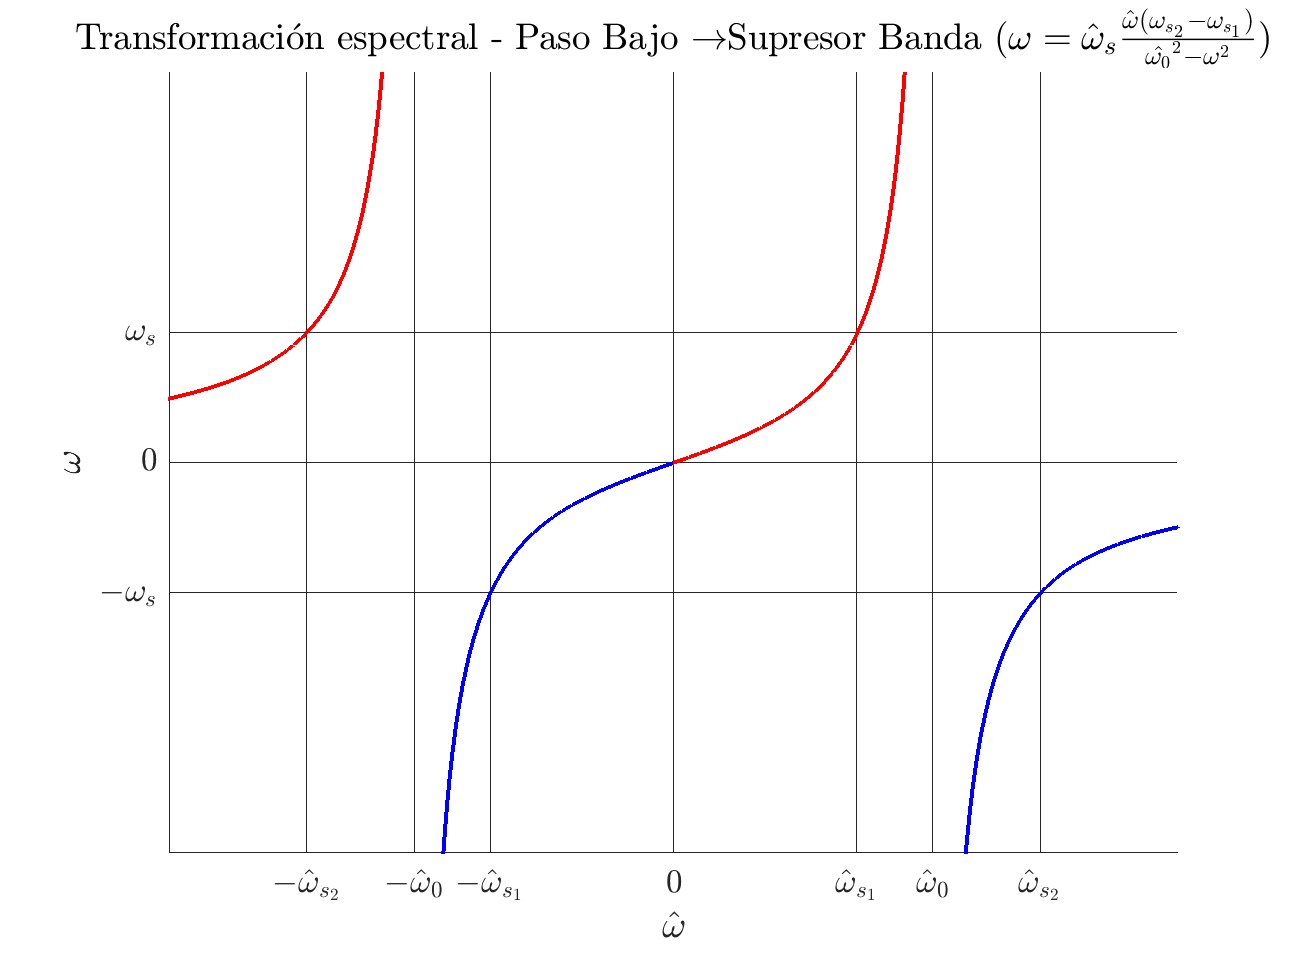
\includegraphics[height=4cm]{Figures/TE_3a.png}\\
  \end{column}
\end{columns}
\begin{center}
  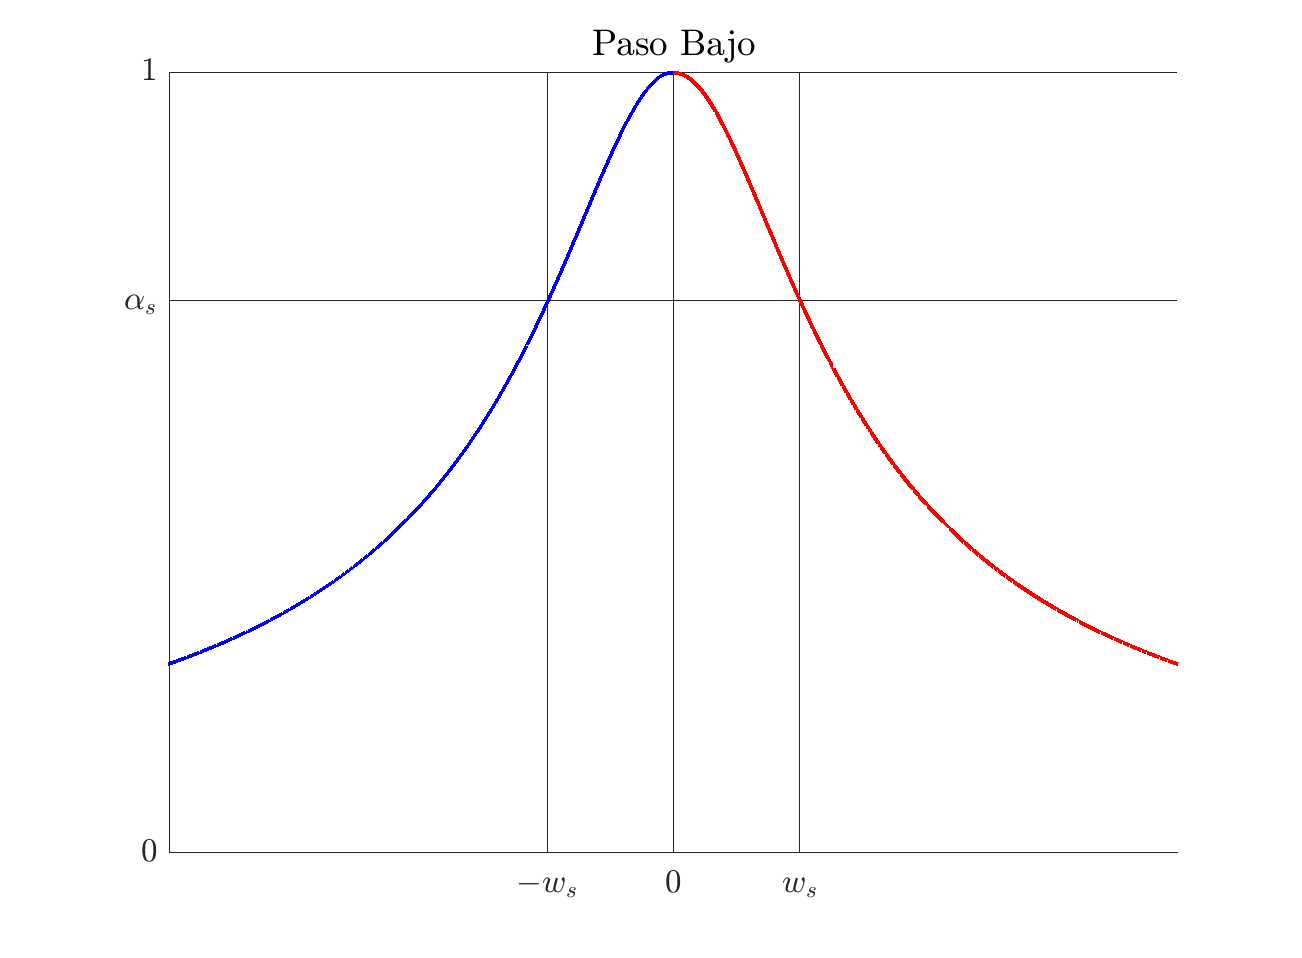
\includegraphics[height=4.25cm]{Figures/TE_3b.png}%
  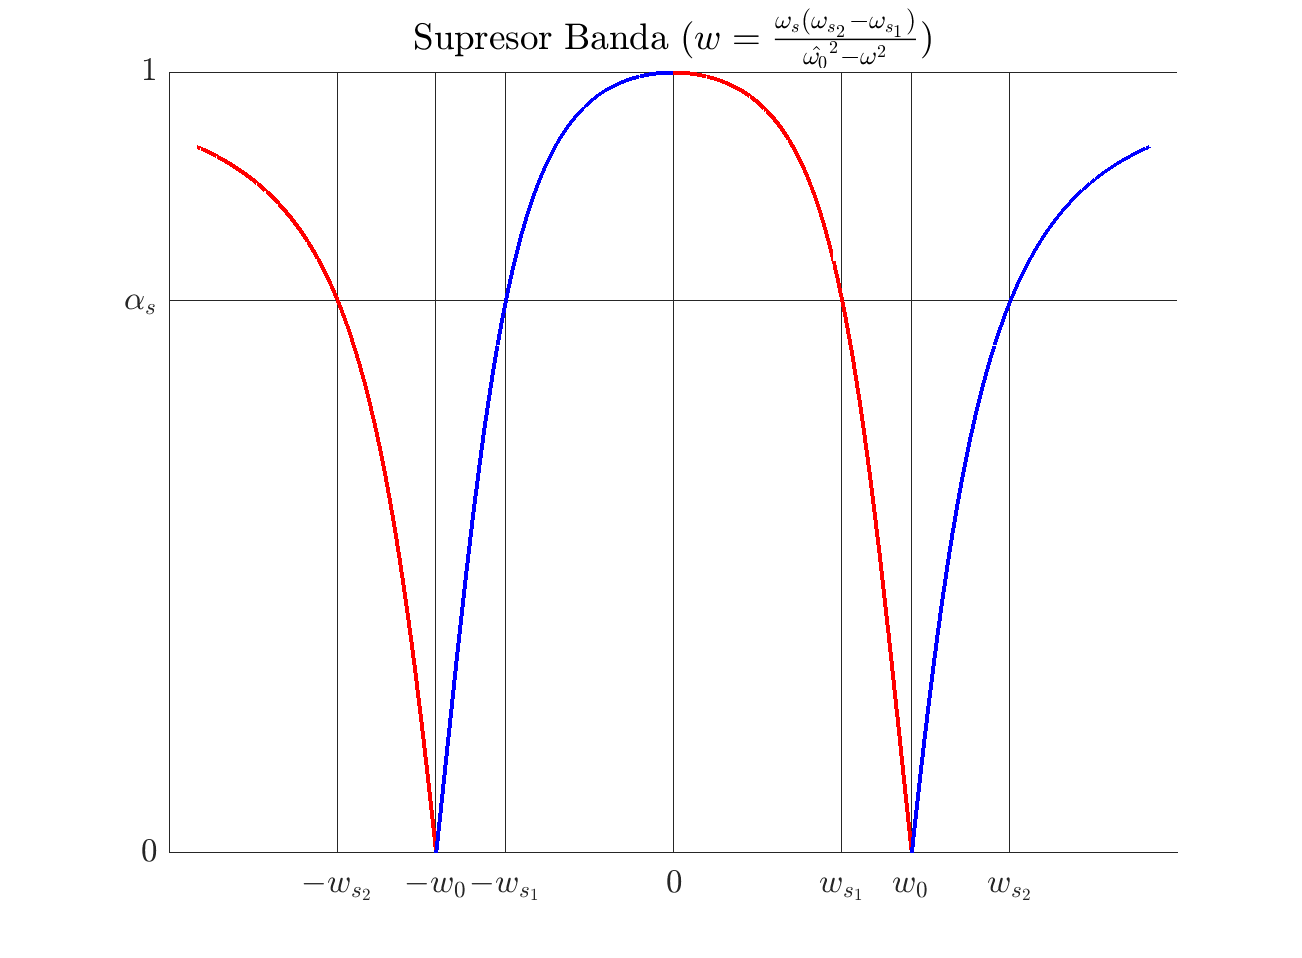
\includegraphics[height=4.25cm]{Figures/TE_3c.png}
\end{center}
\end{frame}


\begin{frame}
\frametitle{Ejemplo filtro paso alto continuo}

\footnotesize

\color{olivegreen}Diseñar un filtro de Butterworth paso altas con un borde paso banda a 4KHz, borde supresor de banda a 1KHz, rizo paso banda de 0.1dB y atenuación supresora de banda mínima 40dB.

\color{gray}
\begin{itemize}
\item $\left . \begin{array}{l}\hat \omega_p=2\pi \cdot 4000\\ \hat \omega_s=2\pi \cdot 1000\end{array}\right \}$ Suponemos $\omega_p=1 \rightarrow \omega_s=-\frac{\omega_p \hat \omega_p}{\hat \omega_s}=-4 $

\item Diseñar el filtro paso bajo con las ordenes correspondientes de Matlab

\item Convertir el filtro paso bajo a paso alta, con la relación espectral o la orden de Matlab  \alert{\texttt{[num,den]=lp2hp(num,den,$\hat{w}_p$)}}.

\end{itemize}

\begin{columns}[c]
\begin{column}{5.1cm}
\vspace{-0.5cm}
\lstinputlisting{./Matlab/ButterCode.m}
\end{column}
\begin{column}{4cm}
\vspace{0.1cm}
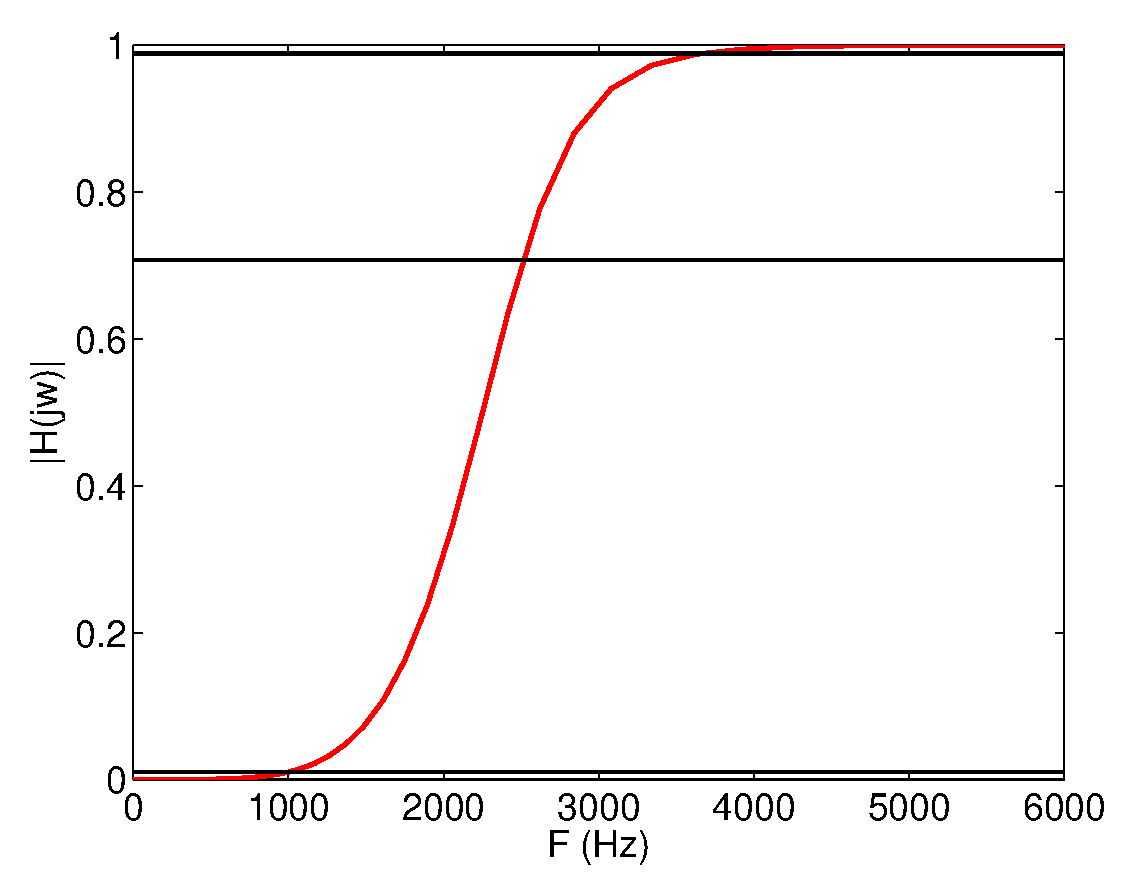
\includegraphics[width=4cm]{./Figures/FiltroButterPA.eps}
\end{column}
\end{columns}

\end{frame}


%%%%%%%%%%%%%%%%%%%%%%%%%%%%%%%%%%%%%%%%%%%%


\begin{frame}
\frametitle{Ejemplo filtro paso banda continuo}

\vspace{-0.1cm}

\footnotesize

\color{olivegreen}Diseñar un filtro elíptico con borde de la banda de paso a 4KHz y 7KHz, bordes supresores de banda a 3KHz y 8KHz, rizo de la banda de paso 1dB y atenuación superiora de banda mínima a 22dB.

\vspace{-0.1cm}

\color{gray}
\begin{itemize}

\scriptsize
\item $\left . \begin{array}{ll}\hat \omega_{p1}=2\pi \cdot 4000 & \hat \omega_{p2}=2\pi \cdot 7000\\\hat \omega_{s1}=2\pi \cdot 3000 & \hat \omega_{s2}=2\pi \cdot 8000\end{array}\right \}$ $\begin{array}{l}\omega_0^2=(2\pi)^2 \cdot 28 \cdot 10^6\\ \omega_0^2=(2\pi)^2 \cdot 24 \cdot 10^6\end{array} $



$\omega_0^2\!=\!(2\pi)^2 \!\cdot \!24 \!\cdot 10^6 \rightarrow  \hat \omega_{p1}\!=\!\frac{\omega_0^2}{\omega_{p2}}\!=\!2\pi \frac{24}{7}10^3$ $\rightarrow \hat \omega_{p2}\!-\!\hat \omega_{p1}\!=\!2\pi(7\!-\!\frac{24}{7})10^3 \!=\!2\pi \frac{25}{7}10^3 $

\vspace{-0.1cm}

Suponemos $\omega_p=1 \rightarrow \omega_s=\omega_p\frac{\hat w^2-\hat \omega_0^2}{\hat w (\hat \omega_{p2}-\hat \omega_{p1})}=\frac{9-24}{3(7-24/7)}=-1.4$

 \footnotesize

\item Diseñar el filtro paso bajo con las ordenes correspondientes de Matlab

\item Convertir el filtro paso bajo a paso alta, con la relación espectral o la orden de Matlab  \alert{\texttt{[num,den]=lp2bp(num,den,$\hat{w}_0$,$\hat{w}_{p2}-\hat \omega_{p1}$)}}.

\end{itemize}

\vspace{-0.1cm}

\begin{columns}[c]
\begin{column}{5.1cm}
\vspace{-0.5cm}
\lstinputlisting{./Matlab/EllipCode.m}
\end{column}
\begin{column}{4cm}
\vspace{0.1cm}
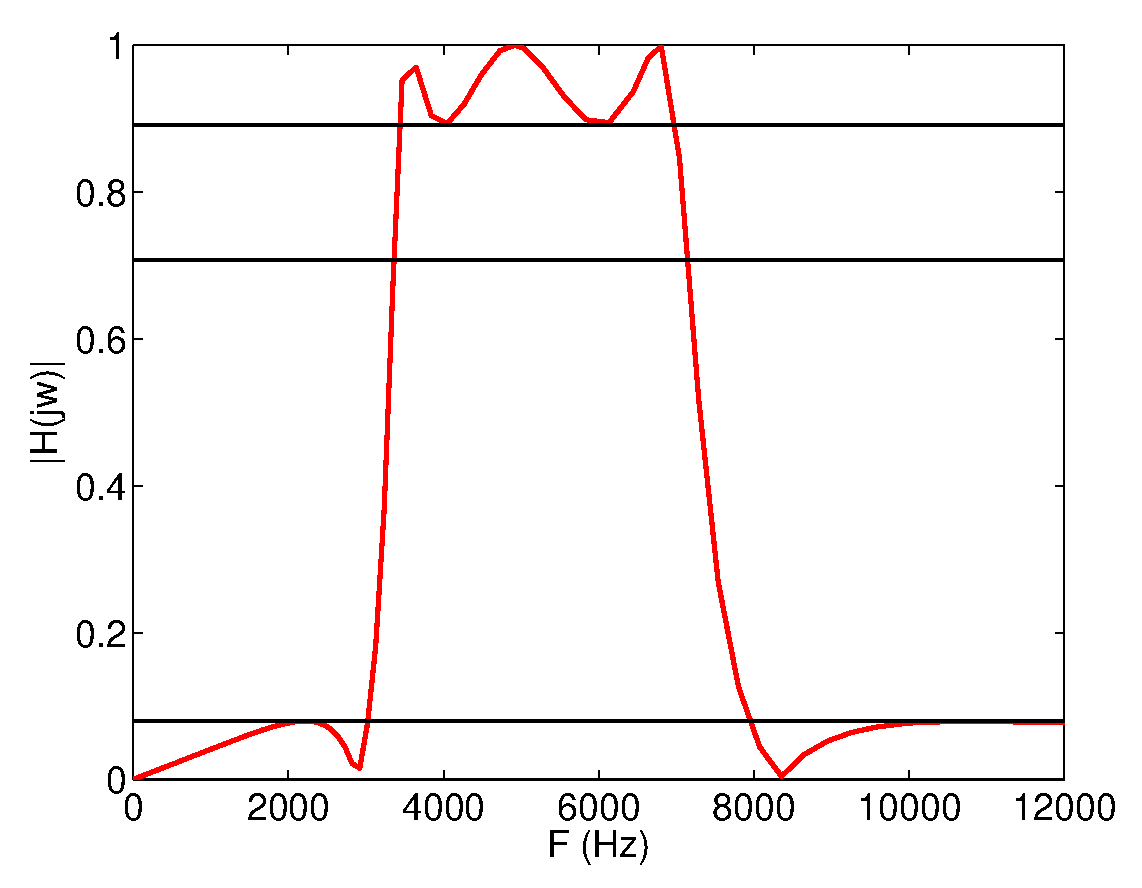
\includegraphics[width=4cm]{./Figures/FiltroEllipPB.eps}
\end{column}
\end{columns}

\end{frame}


%%%%%%%%%%%%%%%%%%%%%%%%%%%%%%%%%%%%%%%%%%%%

\begin{frame}
\frametitle{Ejemplo filtro supresor de banda continuo}

\vspace{-0.1cm}

\footnotesize

\color{olivegreen}Diseñar un filtro de Chebyshev tipo II con borde de la banda de paso a 4KHz y 7KHz, bordes supresores de banda a 5KHz y 6KHz, rizo de la banda de paso 2dB y atenuación superiora de banda mínima a 30dB.

\vspace{-0.1cm}

\color{gray}
\begin{itemize}

\scriptsize
\item $\left . \begin{array}{ll}\hat \omega_{p1}=2\pi \cdot 4000 & \hat \omega_{p2}=2\pi \cdot 7000\\\hat \omega_{s1}=2\pi \cdot 5000 & \hat \omega_{s2}=2\pi \cdot 6000\end{array}\right \}$ $\begin{array}{l}\omega_0^2=(2\pi)^2 \cdot 28 \cdot 10^6\\ \omega_0^2=(2\pi)^2 \cdot 30 \cdot 10^6\end{array} $



$\omega_0^2\!=\!(2\pi)^2 \!\cdot \!28 \!\cdot 10^6 \rightarrow  \hat \omega_{s1}\!=\!\frac{\omega_0^2}{\omega_{s2}}\!=\!2\pi \frac{28}{6}10^3$ $\rightarrow \hat \omega_{s2}\!-\!\hat \omega_{s1}\!=\!2\pi(6\!-\!\frac{28}{6})10^3 \!=\!2\pi \frac{8}{6}10^3 $

\vspace{-0.1cm}

Suponemos $\omega_s=1 \rightarrow \omega_p=\omega_s\frac{\hat \omega_p (\hat \omega_{s2}-\hat \omega_{s1})}{\hat \omega_0^2-\hat \omega_p^2}=\frac{4(6-28/6)}{28-16}=0.44$

 \footnotesize

\item Diseñar el filtro paso bajo con las ordenes correspondientes de Matlab

\item Convertir el filtro paso bajo a paso alta, con la relación espectral o la orden de Matlab  \alert{\texttt{[num,den]=lp2bs(num,den,$\hat{w}_0$,$\hat{w}_{s2}-\hat \omega_{s1}$)}}.

\end{itemize}

\vspace{-0.1cm}

\begin{columns}[c]
\begin{column}{5.1cm}
\vspace{-0.5cm}
\lstinputlisting{./Matlab/ChebyCode.m}
\end{column}
\begin{column}{4cm}
\vspace{0.1cm}
\includegraphics[width=4cm]{./Figures/FiltroChebySB1.eps}
\end{column}
\end{columns}

\end{frame}


%%%%%%%%%%%%%%%%%%%%%%%%%%%%%%%%%%%%%%%%%%%%


\begin{frame}
\frametitle{Filtro continuos con Matlab}

\footnotesize
\begin{itemize}
\item Alternativamente se puede hacer todo en un único paso con las funciones de Matlab que ya conocemos.
\item Veamos un ejemplo con las de Chebyshev de tipo II
\begin{itemize}
\item \alert{\texttt{[N,wn]=cheb2ord(wp,ws,alphap,alphas,'s');}}

\vspace{0.1cm}

{\footnotesize
\hspace{0.5cm}Paso bajo: wp=3, ws=5;

\vspace{0.1cm}

\hspace{0.5cm}Paso alto: wp=5, ws=3;

\vspace{0.1cm}

\hspace{0.5cm}Paso banda: wp=[5 7], ws=[4 8];

\vspace{0.1cm}

\hspace{0.5cm}Eliminación de banda: wp=[5 7], ws=[5.5 6.5];}

\vspace{0.1cm}

\item\alert{\texttt{[num,den]=cheby2(N,alphas,wn,tipo,'s');}}

\vspace{0.1cm}

\hspace{0.5cm}tipo: 'low', 'high', nada, 'stop'
\end{itemize}

\end{itemize}

\end{frame}

%%%%%%%%%%%%%%%%%%%%%%%%%%%%



\begin{frame}
\frametitle{Ejemplos de filtros continuos con Matlab I}

\vspace{-0.1cm}

\footnotesize

\color{olivegreen}Diseñar un filtro de Butterworth paso altas con un borde paso banda a 4KHz, borde supresor de banda a 1KHz, rizo baso banda de 0.1dB y atenuación supresora de banda mínima 40dB.

\vspace{-0.15cm}

\color{gray}

\begin{columns}[c]
\begin{column}{6cm}
\vspace{-0.5cm}
\lstinputlisting{./Matlab/ButterCode2.m}
\end{column}
\begin{column}{4cm}
\vspace{0.1cm}
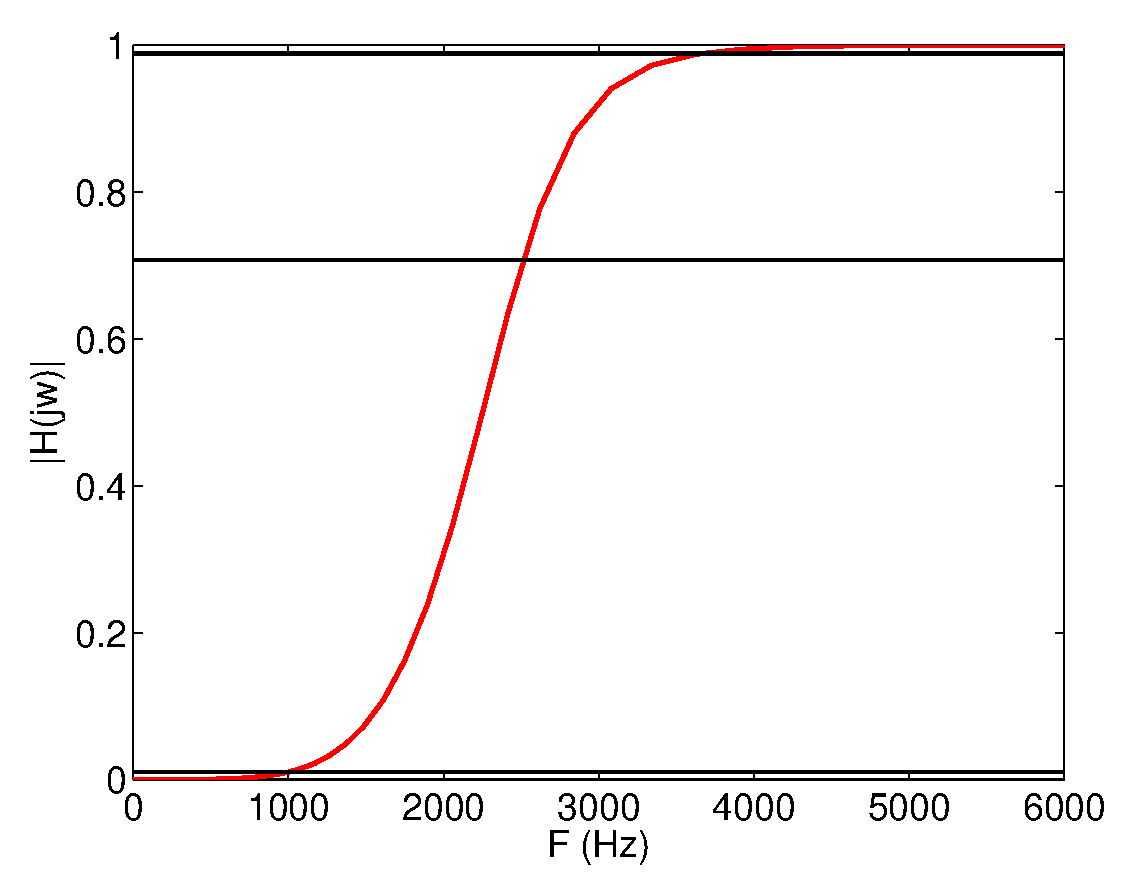
\includegraphics[width=3.8cm]{./Figures/FiltroButterPA.eps}
\end{column}
\end{columns}

\vspace{-0.15cm}

\color{olivegreen}Diseñar un filtro elíptico con borde de la banda de paso a 4KHz y 7KHz, bordes supresores de banda a 3KHz y 8KHz, rizo de la banda de paso 1dB y atenuación superiora de banda mínima a 22dB.

\vspace{-0.1cm}

\color{gray}

\begin{columns}[c]
\begin{column}{6cm}
\vspace{-0.5cm}
\lstinputlisting{./Matlab/EllipCode2.m}
\end{column}
\begin{column}{4cm}
\vspace{0.1cm}
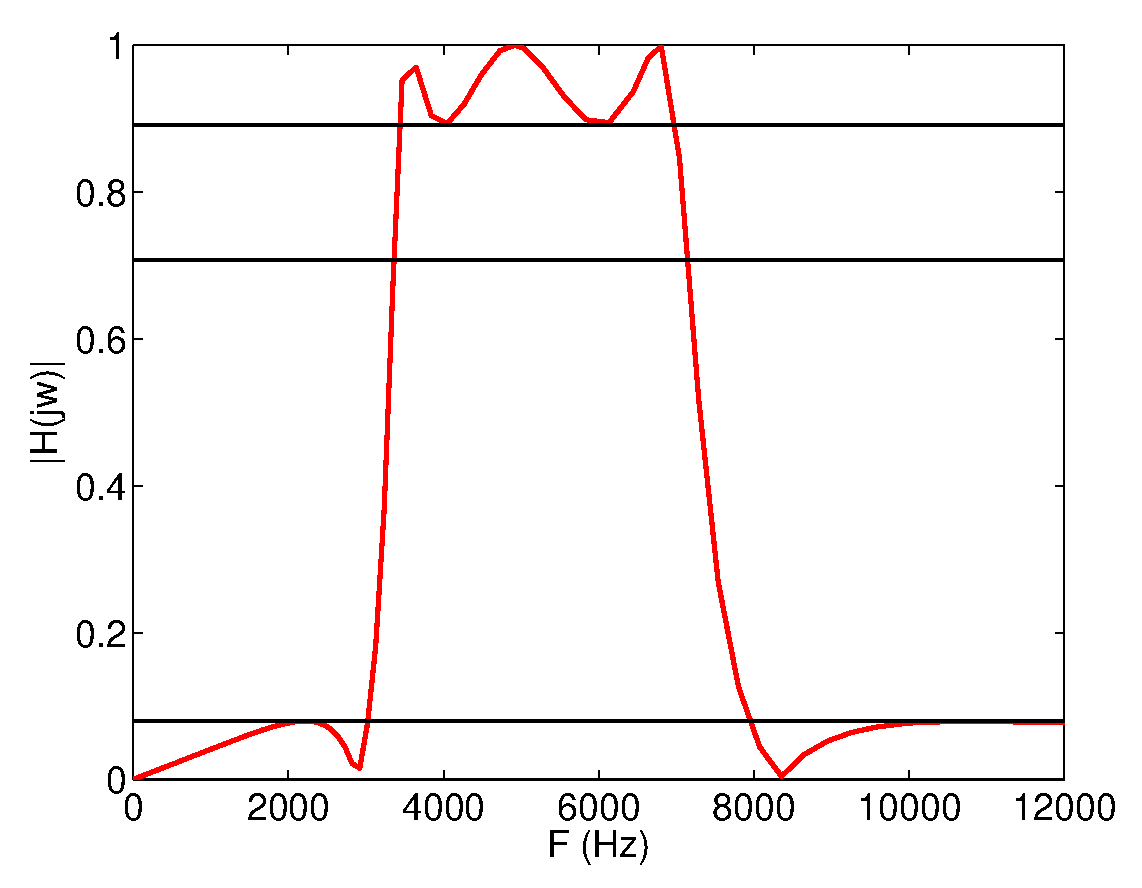
\includegraphics[width=3.8cm]{./Figures/FiltroEllipPB.eps}
\end{column}
\end{columns}

\end{frame}

%%%%%%%%%%%%%%%%%%%%%%%%%%%%%%%%%%%%%%%%%%%%%%%%


\begin{frame}
\frametitle{Ejemplos de filtros continuos con Matlab II}

\vspace{-0.1cm}

\footnotesize

\color{olivegreen}Diseñar un filtro de Chebyshev tipo I supresor de banda con borde de la banda supresora de 2 KHz a 6 KHz, borde de la banda de paso de 1KHz a 7 KHz, rizo baso banda de 0.5dB y atenuación supresora de banda mínima 20dB.

\vspace{0.2cm}


\color{gray}

\begin{columns}[c]
\begin{column}{6cm}
\vspace{-0.5cm}
\lstinputlisting{./Matlab/ChebyCode2.m}
\end{column}
\begin{column}{4cm}
\vspace{0.1cm}
\includegraphics[width=3.8cm]{./Figures/FiltroChebySB.eps}
\end{column}
\end{columns}

\vspace{-0.15cm}



\end{frame}

%%%%%%%%%%%%%%%%%%%%%%%%%%%%%%%%%%%%%%%%%%%%%%%%

% 
\section{Filtros Discretos}


\subsection{Filtros IIR}

\begin{frame}
\frametitle{Procedimiento de diseño de filtros IIR}

\footnotesize

\begin{itemize}
\item Diseño a partir de las aproximaciones de filtros analógicos:

\hspace{2.5cm}\alert{$H_a(s)=\frac{N_a(s)}{D_a(s)}  \:\:\: \rightarrow \:\:\:   H(z)=K \frac{N(z)}{D(z)}$}
\visible<2->{
\begin{itemize}
\footnotesize
\item Aprovechan los avances existentes en la definición de los filtros analógicos (y la existencia de tablas/programas que permiten definirlos)
\item Suelen producir soluciones con forma cerrada (la expresión matemática de la función de transferencia)
\item El procedimiento sirve también para simular el comportamiento de los filtros analógicos antes de construirlos.
\item En algunos casos es necesario normalizar H(z) ya que en la conversión no se conserva que la magnitud máxima sea igual a 1.
\end{itemize}}
\visible<3->{
\item De forma asistida por computador, utilizando algoritmos que optimicen la posición de los polos/ceros del filtro. La optimización suele consistir en minimizar el error entre la respuesta en frecuencia deseada y la del filtro diseñado. Se utiliza para diseñar filtros con prestaciones particulares.
}

\end{itemize}
\end{frame}

%%%%%%%%%%%%%%%%%%%%%%%


\begin{frame}
\frametitle{Transformación del espacio de trabajo ($s \leftrightarrow z$)}
\footnotesize

\begin{itemize}

\item \alert{Filtro continuo $H_a(s)$ $\rightarrow$  filtro discreto: $H(z)=H_a(s)|_{s=F(z)}$}

\visible<2->{
\item Existen diferentes tipos de funciones $s=F(z)$:}

\begin{itemize}
\footnotesize



\visible<3->{
\item \alert{Relación a la respuesta al impulso: $z=e^{Ts}$}
\vspace{-0.2cm}
\begin{columns}[c]
\hspace{1cm}\begin{column}{7cm}
\begin{itemize}
\scriptsize
\item Asigna bandas de anchura $2\pi/T$ en el plano s negativo con puntos dentro la circunferencia unidad en el plano z. Este hecho esta relacionado con el fenómeno del aliasing.

\item Es una correspondencia de muchos (continuo) a uno (discreto).

\item Debido al aliasing, solo sirve para diseñar filtros paso baja y paso banda.

\end{itemize}
\end{column}
\hspace{-0.5cm}\begin{column}{3.5cm}
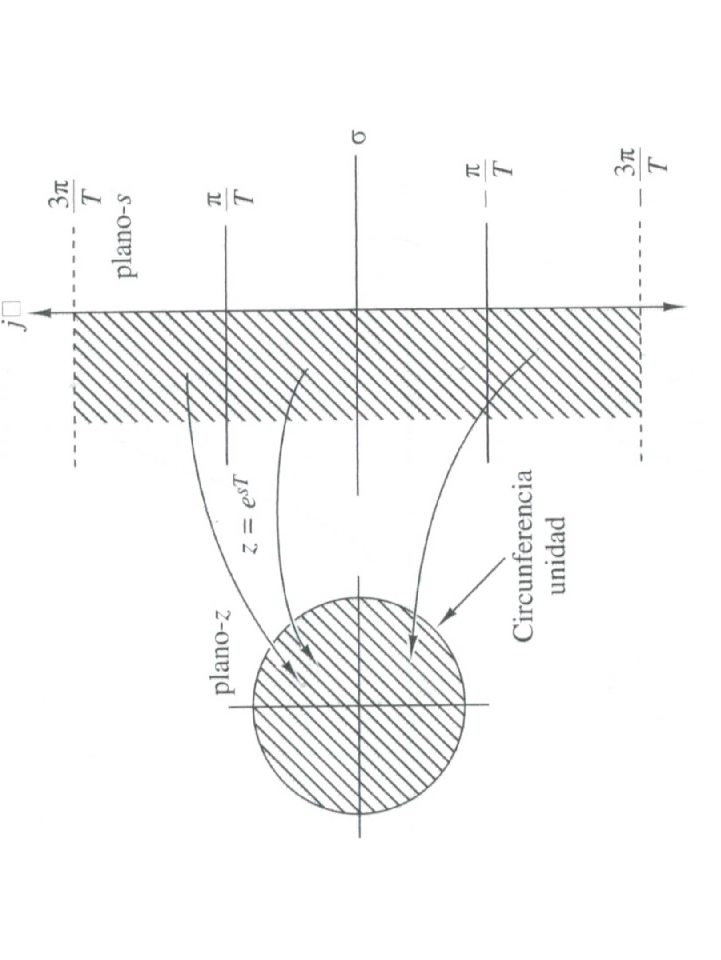
\includegraphics[trim=0cm 1cm 0cm 1cm, clip=true,angle=-90,width=3.5cm]{Figures/Impulso.png}
\end{column}
\end{columns}
}
\visible<4->{
\item \alert{Aproximación por derivadas: $\:\:s= \frac{1-z^{-1}}{T} \: \: \leftrightarrow \:\: z=\frac{1}{1-T\cdot s}$}


\vspace{-0.1cm}
\begin{columns}[c]
\hspace{1cm}\begin{column}{7cm}
\begin{itemize}
\scriptsize
\item Se obtiene sustituyendo la $df(t)/dt$ por $[f(nT)-f((n-1)T)]/T$
\item Puntos del semiplano izquierdo s se relacionan con los puntos internos de la circunferencia pequeña. Se mantiene la estabilidad.
\item Los polos del filtro digital están confinados en la circunferencia pequeña: no se puede diseñar cualquier filtro digital.
\end{itemize}
\end{column}
\hspace{-0.5cm}\begin{column}{3.5cm}
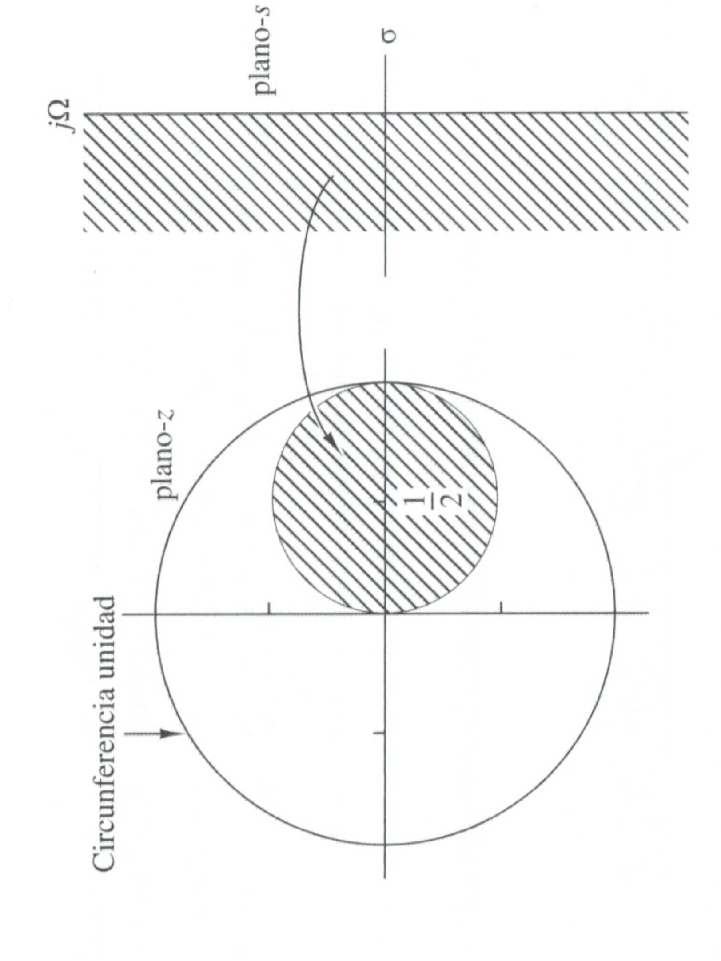
\includegraphics[angle=-90,width=3.5cm]{Figures/Derivada.png}
\end{column}
\end{columns}}
\end{itemize}
\end{itemize}

\end{frame}




%%%%%%%%%%%%%%%%%%%%%%%

\begin{frame}
\frametitle{Transformación del espacio de trabajo ($s \leftrightarrow z$)}
\footnotesize

\begin{itemize}
\item \alert{Filtro continuo $H_a(s)$ $\rightarrow$  filtro discreto: $H(z)=H_a(s)|_{s=F(z)}$}
\item \alert{Transformada bilineal: $\:\:s=\frac{2}{T}\left ( \frac{1-z^{-1}}{1+z^{-1}}\right) \: \: \leftrightarrow \:\: z=\frac{1+T\cdot s/2}{1-T\cdot s/2}$}
\vspace{-0.2cm}
\begin{columns}[T]
\hspace{1cm}\begin{column}{7.5cm}
\begin{itemize}
\scriptsize
\item Se obtiene mediante la aplicación del método de integración numérica trapezoidal a la representación de la ecuación diferencial correspondiente a $H_a(s)$. T es el periodo del paso de integración.

\item Puntos del semiplano izquierdo s se relacionan con los puntos internos a la circunferencia.

\end{itemize}
\end{column}
\begin{column}{4cm}
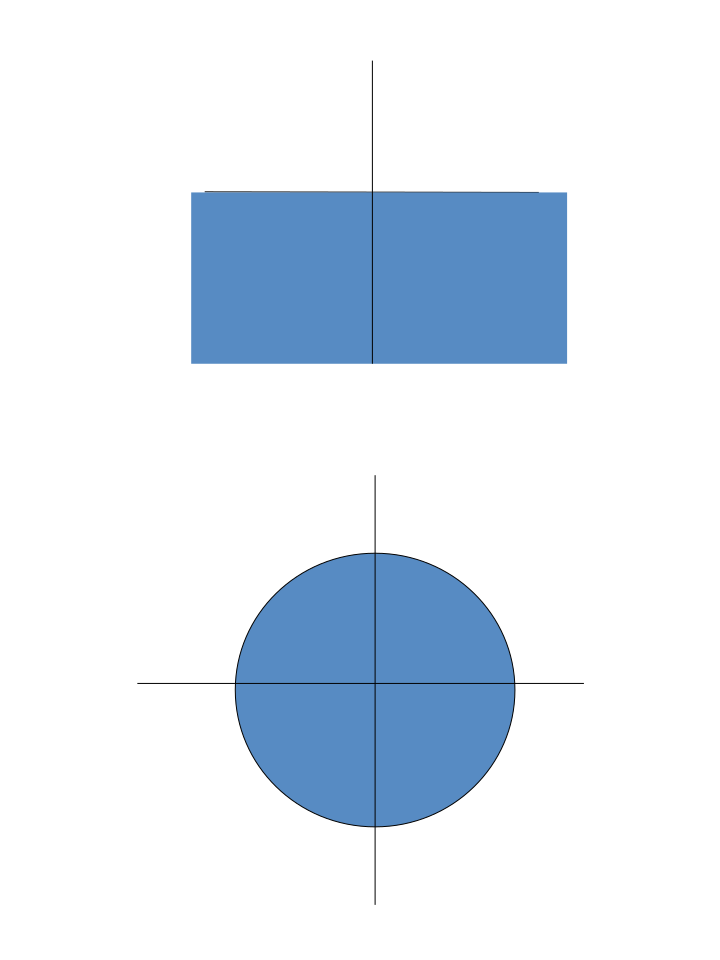
\includegraphics[trim=0cm 0cm 0cm 0cm, clip=true,angle=-90,width=3.5cm]{Figures/Bilineal.png}
\end{column}
\end{columns}


\begin{columns}[T]
\hspace{0.4cm}\begin{column}{11cm}
\begin{itemize}
\scriptsize
\item Es una transformada punto a punto. Se puede utilizar para todos los filtros.

\visible<2->{

\item Relación en frecuencias: \alert{$w_a=\frac{2}{T}tan(w_d/2)$} permite obtener la caracterización del filtro continuo a partir de la caracterización discreta.

\color{gray}
Se establece la relación de s y z con las frecuencias continuas ($s=jw_a$) y discretas ($z=e^{jw_d}$)

$jw_a=\frac{2}{T}\left ( \frac{1-e^{-jw_d}}{1+e^{-jw_d}}\right)=\frac{2}{T}\left ( \frac{e^{jw_d/2}-e^{-jw_d/2}}{e^{jw_d/2}+e^{-jw_d/2}}\right)=\frac{2}{T} j \frac{sen(w_d/2)}{cos(w_d/2)}=\frac{2j}{T} tan(w_d/2)$

Se cumple que  $w_d \!\in \![0,\pi] \leftrightarrow w_a \!\in\! [0,\infty)$; $w_d  \!\in\! [0,-\pi] \leftrightarrow w_a \!\in\! [0,-\infty)$
}
\visible<3->{
\color{black}
\item Se produce un combado de las frecuencias, asociado al comportamiento no lineal de la tangente.
}
\visible<4->{
\item \alert{Si hacemos T=2, las expresiones se simplifican.}
}
\end{itemize}
\end{column}
\end{columns}

\end{itemize}

\end{frame}



%%%%%%%%%%%%%%%%%%%%%%%

\begin{frame}
\frametitle{Diseño de filtros IIR paso bajo}
\small
\begin{enumerate}
\item Aplicar la relación entre las frecuencias ($w_a=\frac{2}{T}tan(w_d/2)$) para obtener la especificación en frecuencias del filtro continuo.
\item Diseñar el filtro continuo correspondiente (Butterworth, Chebyshev, Elíptico). Obtener su función de transferencia $H_a(s)$.
\item Aplicar la transformada bilineal ($s=\frac{2}{T}\left ( \frac{1-z^{-1}}{1+z^{-1}}\right)$) para obtener la función de transferencia del filtro discreto.
\begin{itemize}
\item Con Matlab: \alert{\texttt{[numz,denz]=bilinear(nums,dens,1/T)}}
\end{itemize}

\item Representar la respuesta en frecuencia del filtro (no hay que normalizarlo).
\begin{itemize}
\item Con Matlab: \alert{\texttt{[Hw,w]=freqz(numz,denz)}}


\end{itemize}

\end{enumerate}

\rule{12cm}{0.4pt}
\footnotesize

T=2 para simplificar las expresiones, hacen de la orden bilineal se llamen con tercer parámetro igual a 0.5.

\end{frame}

%%%%%%%%%%%%%%%%%%%%%%%%%%



\begin{frame}
\frametitle{Ejemplo de diseño de filtro  IIR paso bajo}

\footnotesize
\color{olivegreen} Diseñar un IIR de Butterworth paso bajas que opera con una tasa de muestreo de 200 KHz, con una frecuencia de paso de 25KHz y una frecuencia supresora de 55KHz, con un rizo paso banda que no exceda los 0.5 dB y una atenuación mínima en la banda supresora de 15dB.
\color{gray}
\vspace{0.1cm}

1)  Especificaciones del filtro continuo:

\vspace{0.1cm}

$\left . \begin{array}{l}w_{pd}=w_pT_s=2\pi 25/200=0.25\pi\\w_{sd}=w_sT_s=2\pi 55/200=0.55\pi\end{array}\right \}$ $\rightarrow \left . \begin{array}{l}w_{pa}=tan(w_{pd}/2)=0.4142\\w_{sa}=tan(w_{sd}/2)=1.1708\end{array}\right \}$

\vspace{0.1cm}

2) Cálculo del filtro continuo (utilizando expresiones/Matlab):

\vspace{0.1cm}

\hspace{0.3cm}\texttt{[N,wca]=buttord(0.4142,1.1708,.5,15,'s')}

\vspace{0.1cm}

\hspace{0.3cm}\texttt{[numc,denc]=butter(N,wca,'low','s')};

\vspace{0.1cm}

\begin{columns}[T]
\begin{column}{7cm}
3) Conversión al filtro discreto

\vspace{0.1cm}

\hspace{0.3cm}\texttt{[numd,dend]=bilinear(numc,denc,0.5)}

\vspace{0.1cm}

4) Representación del espectro del filtro:

\vspace{0.1cm}

\hspace{0.3cm}\texttt{[Hw,w]=freqz(numz,denz)}

\vspace{0.1cm}

\hspace{0.3cm}\texttt{plot(w/pi,abs(Hw))}
\end{column}
\begin{column}{4cm}

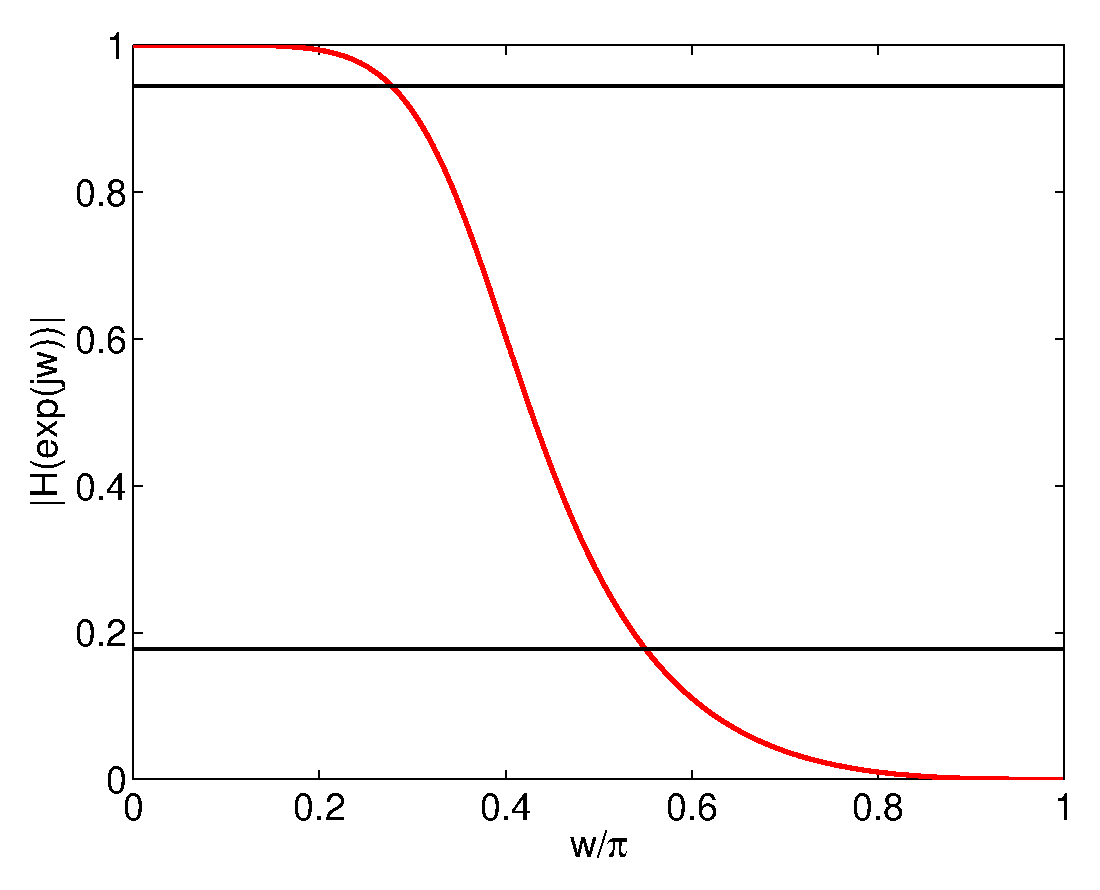
\includegraphics[width=4cm]{Figures/FiltroDiscretoPB_Butter.eps}
\end{column}
\end{columns}


\end{frame}

%%%%%%%%%%%%%%%%%%%%%%%%%%%%


\begin{frame}
\frametitle{Filtros  IIR paso alto, paso banda, supresor de banda}
\small

\visible<2->{
\vspace{-0.4cm}
\begin{enumerate}
\item Aplicar la relación entre las frecuencias ($w_a=\frac{2}{T}tan(w_d/2)$) para obtener la especificación en frecuencias del filtro continuo $H_a(s)$.
\vspace{-0.1cm}
\item Convertir las especificaciones del filtro continuo $H_a(s)$ en las de un filtro paso baja continuo $H_{LP}(s)$.
\vspace{0.1cm}

\begin{columns}[T]
\hspace{0.8cm}\begin{column}{2cm}
\scriptsize
Paso alto:

\vspace{0.2cm}

$s=\frac{w_p \hat w_p}{\hat s}$

\vspace{0.2cm}

 $- w \hat w=w_p \hat w_p$
\end{column}
\hspace{-0.8cm}\begin{column}{3cm}
\scriptsize
Paso banda:

\vspace{0.1cm}

 $s=w_p\frac{\hat s^2+\hat w_0^2}{\hat s (\hat w_{p2}-\hat w_{p1})}$

$w=w_p\frac{\hat w^2-\hat w_0^2}{\hat w (\hat w_{p2}-\hat w_{p1})}$

$\hat w_0^2=\hat w_{p1}\hat w_{p2}=\hat w_{s1}\hat w_{s2}$

\end{column}
\hspace{-0.8cm}\begin{column}{3cm}
\scriptsize
Supresor de banda:

\vspace{0.1cm}

$s=w_s\frac{\hat s (\hat w_{s2}-\hat w_{s1})}{\hat s^2+\hat w_0^2}$

$w=w_s\frac{\hat w (\hat w_{s2}-\hat w_{s1})}{\hat w_0^2-\hat w^2}$

$\hat w_0^2=\hat w_{p1}\hat w_{p2}=\hat w_{s1}\hat w_{s2}$


\end{column}

\end{columns}

\vspace{-0.2cm}

\item Diseñar el filtro continuo paso bajas $H_{LP}(s)$

\vspace{-0.1cm}
}
\visible<4->{
\item Seguir uno de los dos procedimientos siguientes:
}
\end{enumerate}
\vspace{-0.3cm}
\begin{columns}[T]
\begin{column}{5.5cm}
\footnotesize \visible<5->{
\hspace{1.5cm}Procedimiento 1
\begin{itemize}
\scriptsize
\item Convertir el filtro paso baja $H_{LP}(s)$ en el filtro destino $H_a(s)$ usando la relación espectral correspondiente.
\vspace{-0.1cm}
\item  Convertir el filtro $H_a(s)$ en el filtro discreto $H(z)$ con la transformación bilineal ($s=\frac{2}{T}\left ( \frac{1-z^{-1}}{1+z^{-1}}\right)$)
\end{itemize}}
\end{column}
\begin{column}{5.5cm}
\footnotesize \visible<6->{
\hspace{1.5cm}Procedimiento 2
\begin{itemize}
\scriptsize
\item Convertir el filtro paso baja $H_{LP}(s)$ en el filtro $H_{LP}(z)$ con la  transformación bilineal ($s=\frac{2}{T}\left ( \frac{1-z^{-1}}{1+z^{-1}}\right)$).
\vspace{-0.1cm}
\item Convertir el filtro $H_{LP}(z)$ en el filtro destino $H(z)$ usando la relación espectral discreta correspondiente.
\end{itemize}}
\end{column}
\end{columns}
\end{frame}



\begin{frame}
\frametitle{Ejemplo de un filtro  IIR  paso alto}
\footnotesize

\footnotesize
\color{olivegreen} Diseñar con el procedimiento 1 un IIR de Chebyshev Tipo 1 paso altas con las siguientes características: borde de la frecuencia de paso 700Hz, borde de la banda supresora 500Hz, rizo paso banda 1dB, atenuación mínima banda supresora 32 dB, frecuencia de muestreo 2KHz.
\color{gray}
\vspace{0.1cm}

1)  Obtener las especificaciones del filtro continuo paso alta $H_a(s)$:

$\left . \begin{array}{l}w_{pd}=w_pT_s=2\pi 700/2000=0.7\pi\\w_{sd}=w_sT_s=2\pi 500/2000=0.5\pi\end{array}\right \}$ $\rightarrow \left . \begin{array}{l}\hat w_{pa}=tan(w_{pd}/2)=1.9626\\\hat w_{sa}=tan(w_{sd}/2)=1.0\end{array}\right \}$

\vspace{0.1cm}

2) Obtener las especificaciones del filtro continuo paso baja $H_{LP}(s)$:

\vspace{0.1cm}


\hspace{0.25cm}$w\hat w=w_{pa}\hat w_{pa}$. Suponiendo que $w_{pa}=1 \rightarrow w_{sa}=\hat w_{pa}/\hat w_{sa}=1.9626$.

\vspace{0.1cm}

\begin{columns}[T]
 \hspace{0.2cm}\begin{column}{7.7cm}
3) Diseño filtro Chebyshev Tipo 1

\vspace{0.1cm}

\hspace{0.25cm}\texttt{[N,wn]=cheb1ord(1,1.9626,1,32,'s')}

\hspace{0.25cm}\texttt{[numlp,denlp]=cheby1(N,1,wn,'low','s')}

\vspace{0.1cm}

 4) Seguir el procedimiento 1:

 \vspace{0.1cm}

 \hspace{0.25cm}\texttt{[numhp,denhp]=lp2hp(numlp,denlp,1.9626)}

\hspace{0.25cm}\texttt{[numz,denz]=bilinear(numhp,denhp,0.5);}
 \end{column}
 \hspace{-0.5cm}\begin{column}{3.8cm}
 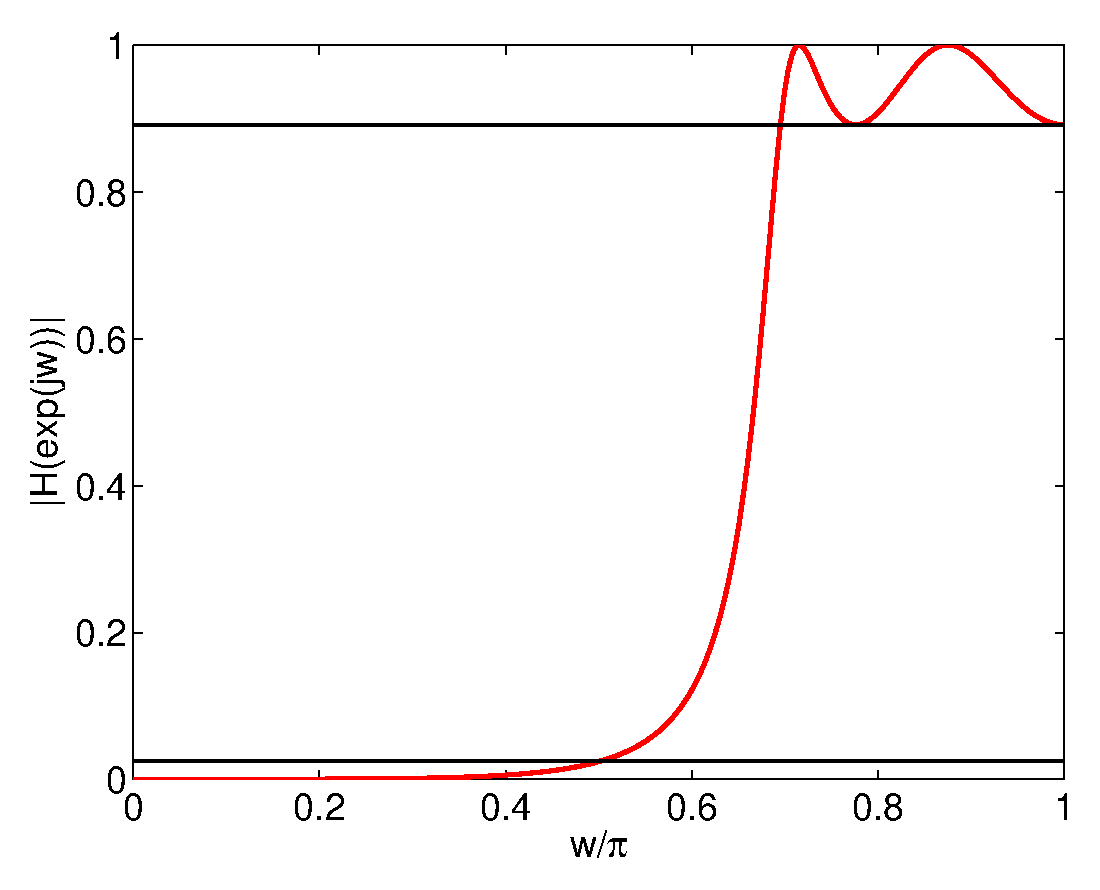
\includegraphics[width=3.8cm]{Figures/FiltroDiscretoPA_Cheby1.eps}
 \end{column}
 \end{columns}

\end{frame}


%%%%%%%%%%%%%%%%%%%%%%%%%%%%%%%%



\begin{frame}
\frametitle{Ejemplo de un filtro  IIR paso banda}
\footnotesize

\footnotesize
\color{olivegreen} Diseñar con el procedimiento 1 un IIR de Butterworth paso banda con las siguientes características: bordes normalizados de la banda de paso 0.45$\pi$ y 0.65$\pi$, bordes normalizados de la banda supresora 0.3$\pi$ y 0.75$\pi$, rizo paso banda 1dB, atenuación mínima banda supresora 40 dB.
\color{gray}
\vspace{0.1cm}

1)  Características del filtro continuo paso banda $H_a(s)$, usando $\hat w_{a}=tan(w_{d}/2)$  :

$\begin{array}{ll}w_{p1d}=0.45\pi \rightarrow \hat w_{p1a}=0.8541 &\:\: w_{p2d}=0.65\pi \rightarrow \hat w_{p2a}=1.6319 \\
w_{s1d}=0.3\pi \rightarrow \hat w_{s1a}=0.5095 &\:\: w_{s2d}=0.75\pi \rightarrow \hat w_{s2a}=2.4142
\end{array}$

\vspace{0.1cm}

2) Obtener las especificaciones del filtro continuo paso baja $H_{LP}(s)$:

\vspace{0.1cm}

$\left . \begin{array}{l}\hat w_0^2 =\hat w_{p1a}\hat w_{p2a}=1.3938\\w_0^2 =\hat w_{s1a}\hat w_{s2a}=1.23
\end{array} \right \}$ $\rightarrow \hat w_{s1a}=\frac{1.3938}{w_{s2a}}=0.5772$, $\hat w_0=1.1806$


\hspace{0.25cm}Si $w_p=1$, $w_{s}=w_p\frac{\hat w_{s1a}^2-\hat w_0^2}{\hat w_{s1a} (\hat w_{p2}-\hat w_{p1})}=2.3617$


\vspace{0.1cm}

\begin{columns}[T]
 \hspace{0.2cm}\begin{column}{7.7cm}
3) Diseño filtro Butterworth

\vspace{0.1cm}

\hspace{0.25cm}\texttt{[N,wn]=buttord(1,2.3617,1,40,'s')}

\hspace{0.25cm}\texttt{[nlp,dlp]=butter(N,wn,'low','s')}

\vspace{0.1cm}

 4) Seguir el procedimiento 1:

 \vspace{0.1cm}
  \hspace{0.28cm}\texttt{banda=1.6139-0.8541;}

 \hspace{0.25cm}\texttt{[npb,dpb]=lp2bp(nlp,dlp,1.1806,banda)}

\hspace{0.25cm}\texttt{[numz,denz]=bilinear(npd,dpd,0.5);}
 \end{column}
 \hspace{-0.5cm}\begin{column}{3.8cm}
 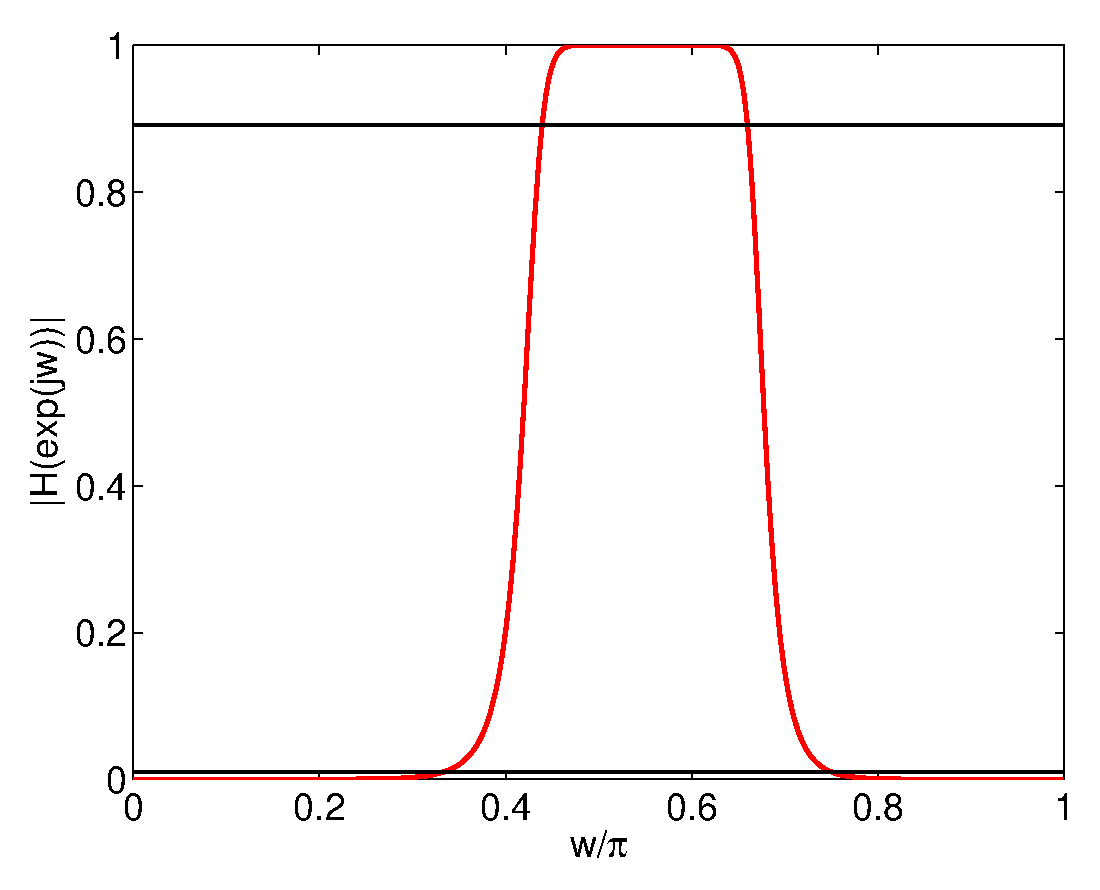
\includegraphics[width=3.8cm]{Figures/FiltroDiscretoPBanda_Butter.eps}
 \end{column}
 \end{columns}

\end{frame}

%%%%%%%%%%%%%%%%%%%%%%%%%%%%%%%%%%%%%%%%%%%%%%%%%%%%%

\begin{frame}
\frametitle{Relaciones espectrales discretas}

\begin{itemize}
\footnotesize
\item La transformación espectral discreta $z=F(\hat z)$ permite obtener a partir de un filtro discreto paso bajo $H_{LP}(z)$  otro filtro discreto$^1$ (paso alto, paso banda, supresor de banda) $H(\hat z)=H_{LP}(z)|_{z=F(\hat z)}$.
\begin{itemize}
\footnotesize

\item Filtro paso alta: $z^{-1}=-\frac{\hat z^{-1}+\lambda}{1+\lambda \hat z^{-1}}$, con
$\lambda=-\frac{cos((w_c-	\hat w_c)/2)}{cos((w_c+	\hat w_c)/2)}$



\item Filtro paso banda: $z^{-1}=-\frac{\hat z^{-2}-\frac{2\lambda \rho}{\rho+1}\hat z^{-1}+\frac{\rho-1}{\rho+1}}{\frac{\rho-1}{\rho+1}\hat z^{-2}-\frac{2\lambda \rho}{\rho+1}\hat z^{-1}+1}$,

$\lambda=\frac{cos((\hat w_{c2}+	\hat w_{c1})/2)}{cos((\hat w_{c2}-	\hat w_{c1})/2)}$, $\rho=\cot((\hat w_{c2}-\hat w_{c1})/2)\tan(w_c/2)$

\item Filtro supresor banda: $z^{-1}=\frac{\hat z^{-2}-\frac{2\lambda}{\rho+1}\hat z^{-1}+\frac{1-\rho}{\rho+1}}{\frac{1-\rho}{\rho+1}\hat z^{-2}-\frac{2\lambda}{\rho+1}\hat z^{-1}+1}$,

$\lambda=\frac{cos((\hat w_{c2}+\hat w_{c1})/2)}{cos((\hat w_{c2}-\hat w_{c1})/2)}$, $\rho=\tan((\hat w_{c2}-\hat w_{c2})/2)\tan(w_c/2)$


\end{itemize}

\item Con Matlab$^{2}$
\begin{itemize}
\footnotesize
\item \texttt{[npa,dpa]=iirlp2hp(numlp,denlp,wplp,wphp)}
\item \texttt{[npa,dpa]=iirlp2bp(numlp,denlp,wplp,[wp1d,wp2d])}
\item \texttt{[nbs,dbs]=iirlp2sp(numlp,denlp,wslp,[ws1d,ws2d])}
\end{itemize}
\end{itemize}

\vspace{-0.2cm}
\rule{10cm}{0.4pt}

\scriptsize
$^1$También existe una relación espectral que permite transformar un filtro paso bajo en otro paso bajo, que se utiliza para cambiar las especificaciones en frecuencia de un filtro paso baja ya diseñado.

$^2$ Las frecuencias tienen que estar  normalizadas entre $[0,1]$ que se corresponden a los valores discretos entre $[0,\pi]$


\end{frame}



\begin{frame}
\frametitle{Ejemplo de un filtro  IIR paso banda}
\footnotesize

\footnotesize
\color{olivegreen} Diseñar con el procedimiento 2 un IIR de Butterworth paso banda con las siguientes características: bordes normalizados de la banda de paso 0.45$\pi$ y 0.65$\pi$, bordes normalizados de la banda supresora 0.3$\pi$ y 0.75$\pi$, rizo paso banda 1dB, atenuación mínima banda supresora 40 dB.
\color{gray}
\vspace{0.1cm}

1)  Características del filtro continuo paso banda $H_a(s)$, usando $\hat w_{a}=tan(w_{d}/2)$  :

$\begin{array}{llll}\hat w_{p1a}=0.8541 &\hat w_{p2a}=1.6319  & \hat w_{s1a}=0.5095 & \hat w_{s2a}=2.4142
\end{array}$

\vspace{0.1cm}

2) Obtener las especificaciones del filtro continuo paso baja $H_{LP}(s)$:

\vspace{0.1cm}

\hspace{0.25cm}$\hat w_{s1a}=\frac{1.3938}{w_{s2a}}=0.5772$, $\hat w_0=1.1806$, $w_p=1$, $w_{s}=2.3617$


\vspace{0.1cm}

\begin{columns}[T]
 \hspace{0.2cm}\begin{column}{7.7cm}
3) Diseño filtro Butterworth

\vspace{0.1cm}

\hspace{0.25cm}\texttt{[N,wn]=buttord(1,2.3617,1,40,'s')}

\hspace{0.25cm}\texttt{[nlp,dlp]=butter(N,wn,'low','s')}

\vspace{0.1cm}

 4) Seguir el procedimiento 2:

 \vspace{0.1cm}

  \hspace{0.25cm}\texttt{[nlpz,dlpz]=bilinear(nlp,dlp,0.5);}

\visible<2->{
  \hspace{0.25cm}\texttt{[Hlpw,w]=freqz(nlpz,dlpz);}

  \hspace{0.25cm}\texttt{plot(w/pi,abs(Hw))}

   \hspace{0.25cm}\texttt{plot(w/pi,10\^ (-1/20)*ones(length(w),1))};

  }

 \visible<3->{
  \hspace{0.25cm}\texttt{a=ginput(1);} \hspace{0.25cm}\texttt{wp=a(1);}}

  \hspace{0.25cm}\texttt{wpasod=[0.45,0.65];}


 \hspace{0.25cm}\texttt{[nz,dz]=irrlp2bp(nlpz,dlpz,wp,wpasod)}


 \end{column}
 \hspace{-0.5cm}\begin{column}{3.8cm}
\only<2-3|handout=0>{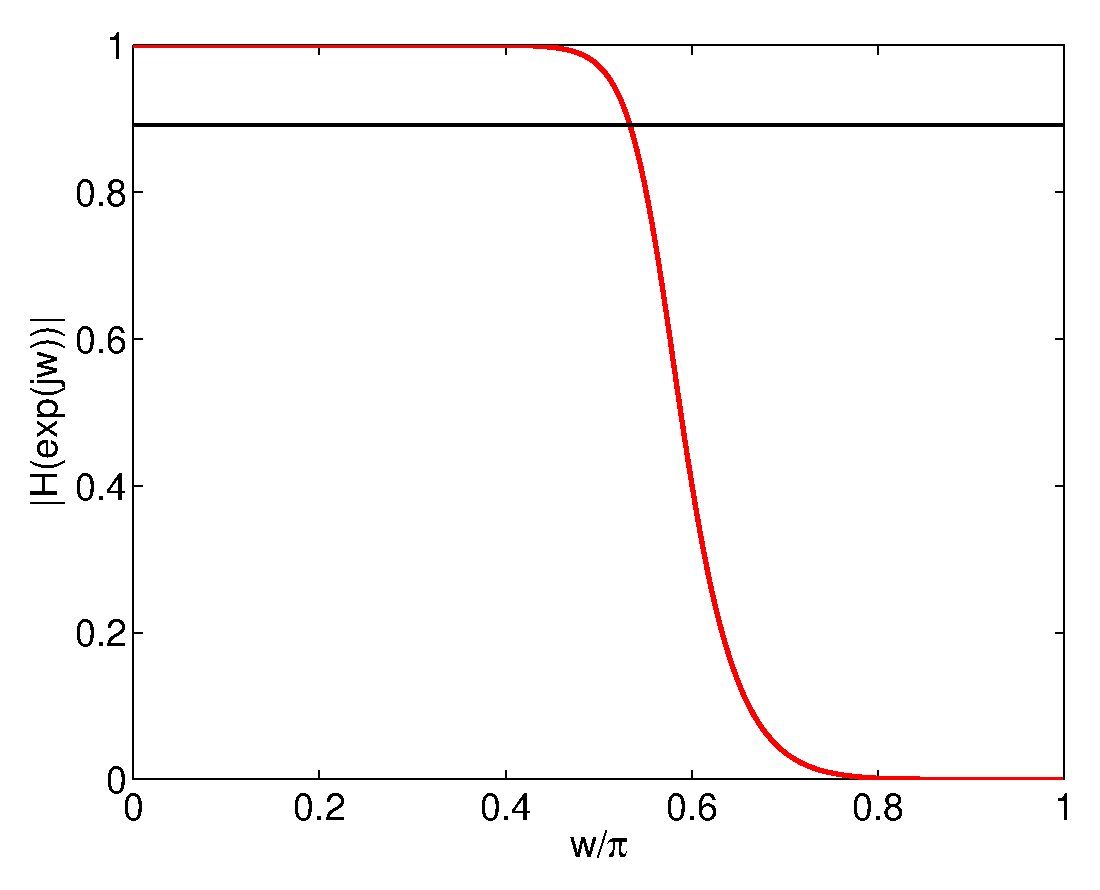
\includegraphics[width=3.8cm]{Figures/FiltroDiscretoPBanda_Butter21.eps}}
\visible<4->{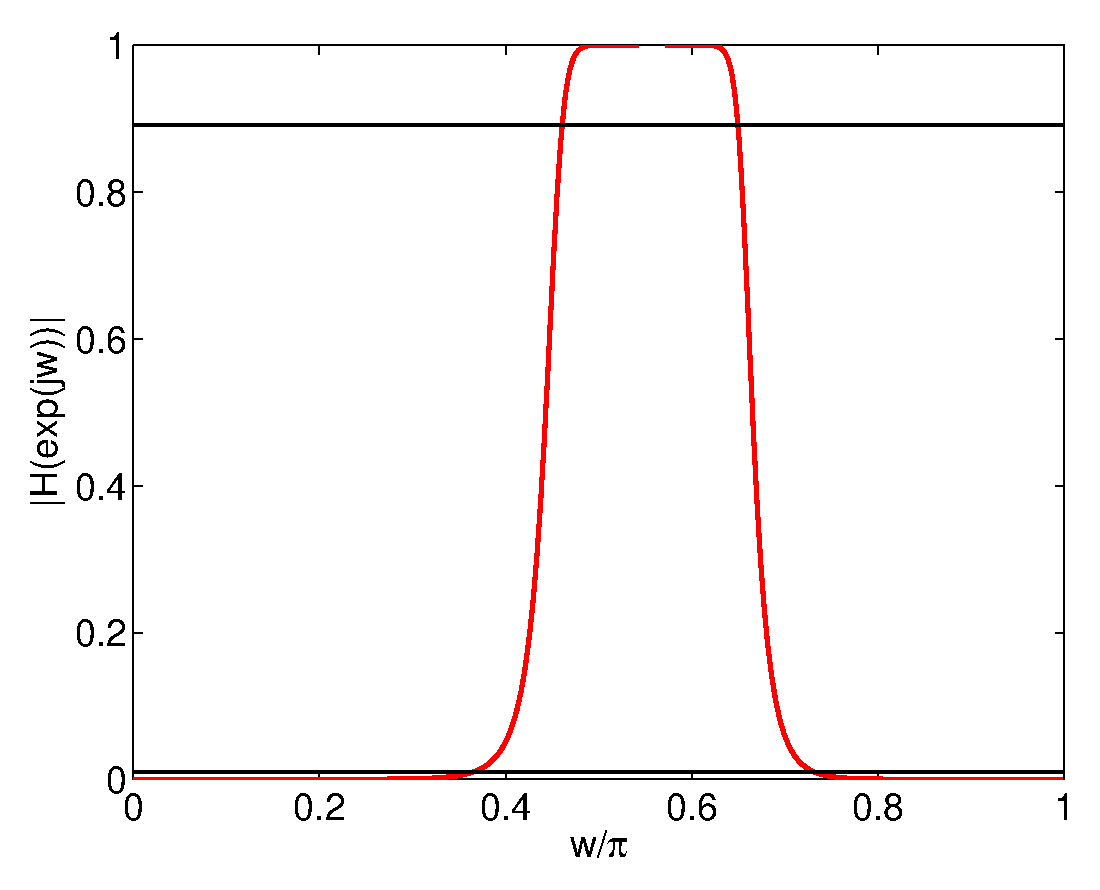
\includegraphics[width=3.8cm]{Figures/FiltroDiscretoPBanda_Butter22.eps}}

 \end{column}
 \end{columns}

\end{frame}

%%%%%%%%%%%%%%%%%%%%%%%%%%%%%%%%%%%%%%%%


\begin{frame}
\frametitle{Diseño de filtros  IIR con Matlab}
\footnotesize
\begin{itemize}
\item Matlab permite realizar directamente el diseño de los filtros discretos, sin necesidad de realizar los pasos intermedios.
\item Para ello, hay que poner en las funciones que ya conocemos las frecuencias normalizadas [0,1] y eliminar la llamada a 's'.

\item Veamos un ejemplo con las funciones de Chebyshev de tipo II
\begin{itemize}
\item \alert{\texttt{[N,wn]=cheb2ord(wp,ws,alphap,alphas);}}

\vspace{0.1cm}

{\footnotesize
\hspace{0.5cm}Paso bajo: wp=0.3, ws=0.5;

\vspace{0.1cm}

\hspace{0.5cm}Paso alto: wp=0.5, ws=0.3;

\vspace{0.1cm}

\hspace{0.5cm}Paso banda: wp=[0.5 0.7], ws=[0.4 0.8];

\vspace{0.1cm}

\hspace{0.5cm}Eliminación de banda: wp=[0.5 0.7], ws=[0.55 0.65];}

\vspace{0.1cm}

\item\alert{\texttt{[num,den]=cheby2(N,alphas,wn,tipo);}}

\vspace{0.1cm}

\hspace{0.5cm}tipo: 'low', 'high', nada, 'stop'

\end{itemize}


\item Los resultados de Matlab coinciden con los obtenidos a través del procedimiento 1.

\end{itemize}

\end{frame}





\begin{frame}
\frametitle{Ejemplo de un filtro  IIR paso banda}
\footnotesize

\footnotesize
\color{olivegreen} Diseñar directamente con Matlab un IIR de Butterworth paso banda con las siguientes características: bordes normalizados de la banda de paso 0.45$\pi$ y 0.65$\pi$, bordes normalizados de la banda supresora 0.3$\pi$ y 0.75$\pi$, rizo paso banda 1dB, atenuación mínima banda supresora 40 dB.
\color{gray}
\vspace{0.1cm}


\vspace{0.1cm}

\begin{columns}[T]
\begin{column}{6cm}
\lstinputlisting{./Matlab/ButterDCode.m}


 \end{column}
\hspace{-0.5cm} \begin{column}{4.5cm}
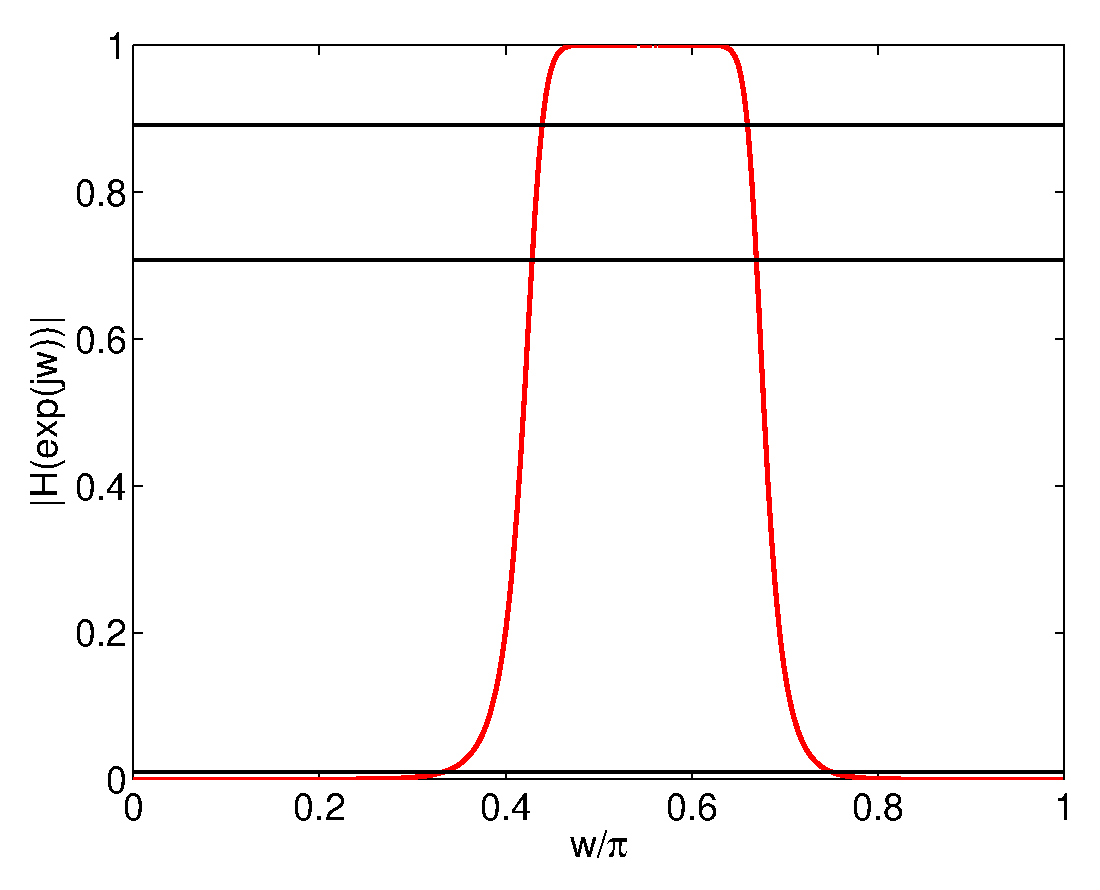
\includegraphics[width=4.5cm]{Figures/FiltroDiscretoPBanda_ButterMatlab.eps}

 \end{column}
 \end{columns}

\end{frame}


\subsection{Filtros FIR}

\begin{frame}
\frametitle{Procedimiento de diseño de filtros FIR}

\begin{itemize}
\footnotesize
\item Los filtros discretos FIR no tienen conexión directa con ningún filtro continuo, y por lo tanto, su diseño no se puede basar en la construcción de ningún filtro analógico.

\visible<2->{\item El diseño de estos filtros se basa en la aproximación directa de la respuesta en frecuencia deseada (i.e. calcular los valores de $h(n)$ para que $H(e^{jw})$ tenga la forma deseada).

\hspace{0.8cm}$H(e^{jw})=\sum_{n=-\infty}^{\infty} h(n)e^{-jwn} \rightarrow H(e^{jw})=\sum_{n=0}^{N} h(n)e^{-jwn} $   }

\visible<3->{
\item Los filtros que vamos a estudiar cumplen dos propiedades adicionales: son filtros con \alert{$h(n)$ real} y \alert{fase lineal} en la respuesta en frecuencia: $arg(H(e^{jw}))=\alpha w+\beta$. Ambos hechos\visible<5->{$^1$} hacen que el desfase sea introducido por el filtro a cada frecuencia sea $-Nw/2$.

\begin{itemize}
\footnotesize
\item Transformada de Fourier con ventana.
\item \color{gray} Muestreo en frecuencia.\color{black}
\item Diseño asistido por computador.
\end{itemize}
}

\visible<4->{
\item Veremos que para diseñar los filtros será necesario primero estimar el valor $N$ y a continuación los valores de las h(n).
}

\end{itemize}

\visible<5->{
\rule{12cm}{0.4pt}
\scriptsize
$^1$ Al final del tema veremos las propiedades que cumplen todos los filtros FIR con $h(n)$ real y fase lineal. En esta sección nos centraremos en el diseño de un subconjunto de estos filtros.}
\end{frame}



\begin{frame}
\frametitle{Diseño FIR por la TF con ventana  }

\vspace{-0.2cm}

\footnotesize


\begin{itemize}
\item La TF en tiempo discreto relaciona la respuesta en frecuencia del filtro con la respuesta del filtro a la señal impulso $h(n)$.  La segunda expresión permite obtener la $h_d(n)$ a partir de la respuesta en frecuencia $H_d(e^{jw})$.



\hspace{1cm}$H_d(e^{jw})=\sum_{n=-\infty}^{\infty}h_d(n)e^{-jwn}$

\hspace{1cm}$h_d(n)=\frac{1}{2\pi}\int_{-\pi}^\pi H_d(e^{jw}) e^{jwn} dw\:\:$  con $\:\:\infty \le n \le \infty$


\end{itemize}

\vspace{-0.3cm}

\visible<2->{

\begin{columns}[c]
\begin{column}{8cm}
\begin{itemize}

\item El problema surge cuando se desea diseñar un filtro cuya respuesta en frecuencia toma un valor constante en módulo por secciones, ya que esto implica que la respuesta a la función impulso es de longitud doblemente infinita (no causal y distinta de cero $\:\:\infty \le n \le \infty$).
\end{itemize}
\end{column}
\hspace{-0.4cm}\begin{column}{3cm}
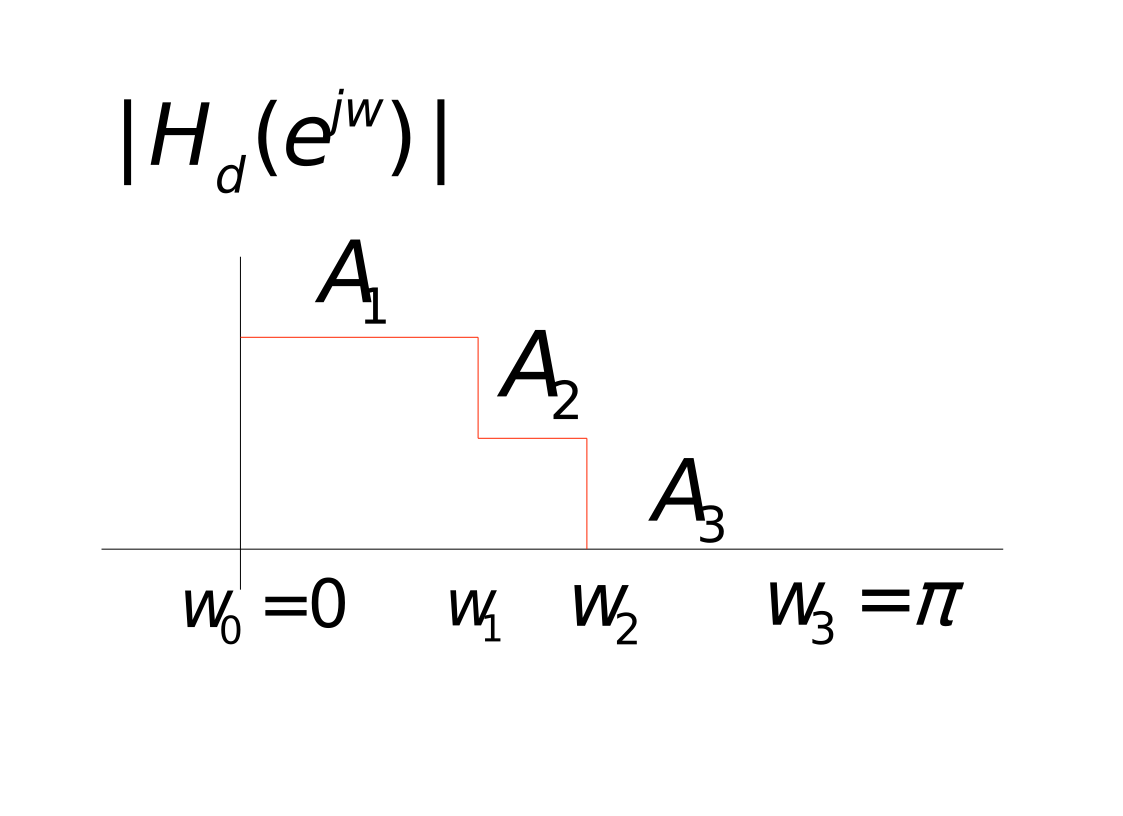
\includegraphics[trim=0cm 1cm 0cm 1cm,clip=true,width=3.5cm]{Figures/PorTramos}
\end{column}
\end{columns}
}

\vspace{-0.1cm}
\begin{itemize}

\visible<3->{
\item Para convertir el filtro deseado $h_d(n)$ en un FIR de orden N+1 podemos:
}

\begin{enumerate}
\footnotesize
\visible<4->{\item Limitar el tamaño de la respuesta al impulso (truncarla/enventanarla,  $h_t(n)=v(n)h_d(n)$) con una ventana $v(n)$ de tamaño 2L+1=N+1.}
\visible<5->{
\item Retardar la respuesta del filtro $L=N/2$ unidades, para convertirlo en causal: $h(n)=h_t(n-L)$. Esto permite que el desfase en frecuencia sea lineal ya que $H(e^{jw})=e^{-jLw}H_t(e^{jw})=e^{-jwN/2}H_t(e^{jw})$.
}
\end{enumerate}
\end{itemize}

\vspace{-0.2cm}

\visible<6->{
\rule{12cm}{0.4pt}
\scriptsize
$h_d(n)$ es el filtro que $d$eseamos diseñar, $h_t(n)$ el sistema  que se obtiene $t$runcando/enventanando $h_d(n)$, y h(n) el filtro FIR (causal) final. }
\end{frame}

%%%%%%%%%%%%%%%%%%%%%%%%%%

\begin{frame}
\frametitle{Respuesta al impulso de filtros deseados I}
\footnotesize

\begin{itemize}
\item Se calcula la $h_d(n)$  de los filtros deseados con $h_d(n)\!=\!\frac{1}{2\pi}\!\!\int_{-\pi}^\pi H_d(e^{jw}) e^{jwn} dw$ o a través de las propiedades de la TFDT.
\end{itemize}

\begin{columns}[T]


\begin{column}{5cm}
\scriptsize
\visible<2->{\centering{
\alert{Filtro paso bajo}}


\vspace{0.1cm}

$\scriptsize H_{LPd}(e^{jw})\!=\!\left \{  \!\!\!\begin{array}{l} 1, \:\:\: |w|\!\!<\!\!w_c\\0,\:\:\: w_c\le |w| \le \pi \end{array}\right .$


\vspace{0.1cm}
\color{gray}$h_{LPd}(n)=\frac{1}{2\pi}\int_{-w_c}^{w_c} e^{jwn}dw$\color{black}


\vspace{0.1cm}
$h_{LPd}(n)=\!\left \{\!\!\!\begin{array}{l}\frac{w_c}{\pi}, \:\:\:  \:\:\: \:\:\: n=0\\ \frac{sen(nw_c)}{\pi n},  \:\:\: c.c.\end{array}  \right . $


\vspace{0.1cm}
}
\visible<3->{
\scriptsize
\centering{
\alert{Filtro paso alto}}

\vspace{0.1cm}
$\scriptsize H_{HPd}(e^{jw})\!=\!\left \{  \!\!\!\begin{array}{l} 0, \:\:\: |w|\!\!<\!\!w_c\\1,\:\:\: w_c\le |w| \le \pi \end{array}\right .$


\vspace{0.1cm}

\color{gray}
$H_{HPd}(e^{jw})=1-H_{LPd}(e^{jw})$

\vspace{0.1cm}

$h_{HPd}(n)=\delta(n)-h_{LPd}(n)$

\color{black}

\vspace{0.1cm}

$h_{HPd}(n)=\!\left \{\!\!\!\begin{array}{l}1-\frac{w_c}{\pi}, \:\:\:  \:\:\: \:\:\: n=0\\ -\frac{sen(nw_c)}{\pi n},  \:\:\: c.c.\end{array}  \right . $

}

\end{column}
\begin{column}{5.5 cm}
\scriptsize
\visible<4->{
\centering{
\alert{Filtro paso banda}}

\vspace{0.1cm}


$\scriptsize H_{BPd}(e^{jw})\!=\!\left \{  \!\!\!\begin{array}{l} 1, \:  w_{1}\!\!<\!\!|w|\!\!<\!\!w_{2}\\0, \:\textrm{c.c.}  \end{array}\right .$


\vspace{0.1cm}
\color{gray}


\vspace{0.1cm}

$H_{BPd}(e^{jw})=H_{HPd,w_1}(e^{jw})-H_{HPd,w_2}(e^{jw})$


\vspace{0.1cm}

\color{black}

$h_{BPd}(n)=\!\left \{\!\!\!\begin{array}{l}\frac{w_2-w_1}{\pi}, \:\:\:  \:\:\: \:\:\: n=0\\ \frac{sen(w_2n)-sen(w_1n)}{\pi n},  \:\:\: c.c.\end{array}  \right . $

}
\vspace{0.1cm}

\visible<5->{
\centering{
\alert{Filtro supresor banda}}

\vspace{0.1cm}


$\scriptsize H_{SPd}(e^{jw})\!=\!\left \{  \!\!\!\begin{array}{l} 0, \:  w_{1}\!\!<\!\!|w|\!\!<\!\!w_{2}\\1, \:\textrm{c.c.}  \end{array}\right .$


\vspace{0.1cm}

\color{gray}
$H_{SPd}(e^{jw})=1-H_{BPd}(e^{jw})$


\vspace{0.1cm}

$h_{SPd}(n)=\delta(n)-h_{BPd}(n)$

\color{black}


\vspace{0.1cm}

$h_{SPd}(n)=\!\left \{\!\!\!\begin{array}{l}1-\frac{w_2-w_1}{\pi}, \:\:\:  \:\:\: \:\:\: n=0\\ -\frac{sen(w_2n)-sen(w_1n)}{\pi n},  \:\:\: c.c.\end{array}  \right . $
}

\end{column}
\end{columns}




\end{frame}

%%%%%%%%%%%%%%%%%%%%%%%%%%

\begin{frame}
\frametitle{Respuesta al impulso de filtros deseados II}
\footnotesize

\begin{itemize}
\item Respuesta al impulso de los diferentes filtros deseados (cuadro resumen en la columna izquierda, filtro multinivel en la columna derecha)
\end{itemize}

\begin{columns}[T]
\begin{column}{5cm}

\scriptsize

\centering{
\alert{Filtro paso bajo}}


\vspace{0.1cm}
$h_{LPd}(n)=\!\left \{\!\!\!\begin{array}{l}\frac{w_c}{\pi}, \:\:\:  \:\:\: \:\:\: n=0\\ \frac{sen(nw_c)}{\pi n},  \:\:\: c.c.\end{array}  \right . $

\vspace{0.1cm}

\centering{
\alert{Filtro paso alto}}



\vspace{0.1cm}

$h_{HPd}(n)=\!\left \{\!\!\!\begin{array}{l}1-\frac{w_c}{\pi}, \:\:\:  \:\:\: \:\:\: n=0\\ -\frac{sen(nw_c)}{\pi n},  \:\:\: c.c.\end{array}  \right . $

\vspace{0.1cm}

\centering{
\alert{Filtro paso banda}}

\vspace{0.1cm}


$h_{BPd}(n)=\!\left \{\!\!\!\begin{array}{l}\frac{w_2-w_1}{\pi}, \:\:\:  \:\:\: \:\:\: n=0\\ \frac{sen(w_2n)-sen(w_1n)}{\pi n},  \:\:\: c.c.\end{array}  \right . $


\vspace{0.1cm}

\centering{
\alert{Filtro supresor banda}}


\vspace{0.1cm}

$h_{SPd}(n)=\!\left \{\!\!\!\begin{array}{l}1-\frac{w_2-w_1}{\pi}, \:\:\:  \:\:\: \:\:\: n=0\\ -\frac{sen(w_2n)-sen(w_1n)}{\pi n},  \:\:\: c.c.\end{array}  \right . $




\end{column}
\hspace{-0.3cm}\begin{column}{6 cm}
\scriptsize

\visible<2->{
\centering{
\alert{Filtro FIR multinivel}}

\vspace{0.1cm}


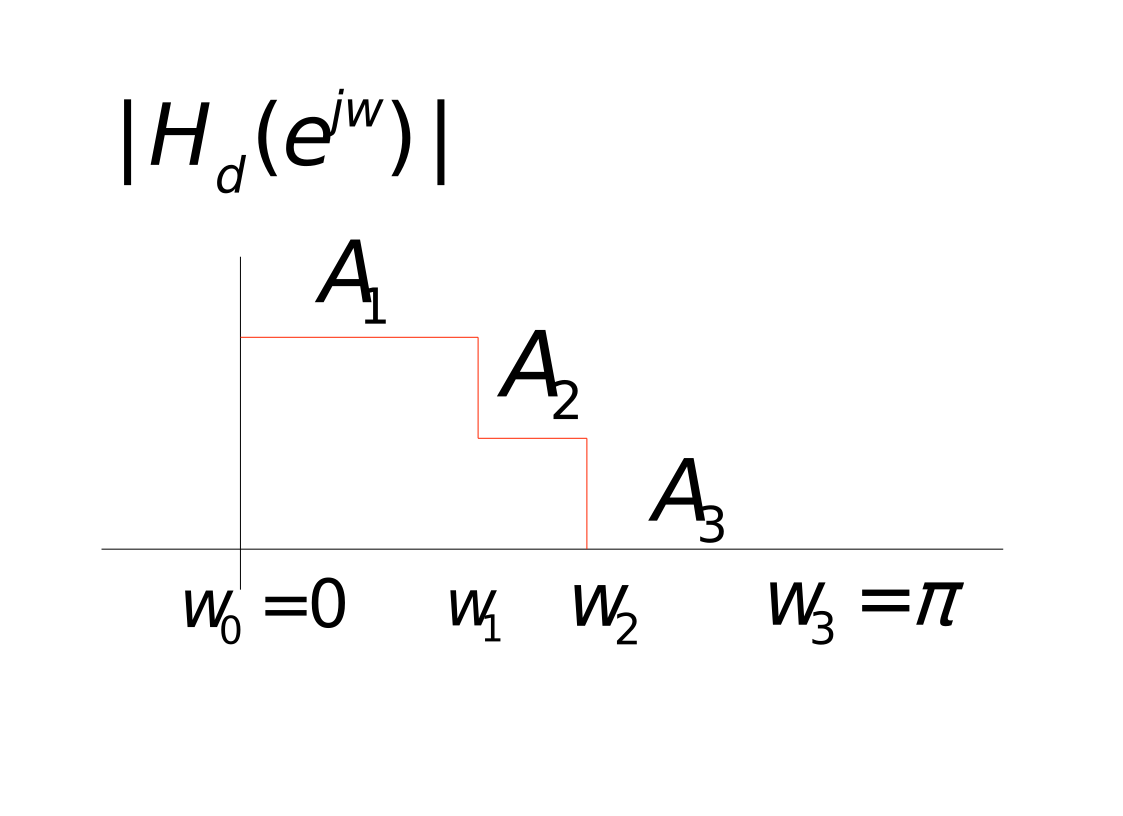
\includegraphics[trim=0cm 1cm 0cm 1cm,clip=true,width=3.5cm]{Figures/PorTramos}


$\scriptsize H_{MNd}(e^{jw})\!=A_k,  \:\:\: w_{k-1}\le|w|\le w_k$

\hspace{1.4cm}$k\!\in\![0,M]$

\hspace{1.0cm}$w_0\!=\!0$

\hspace{1.1cm}$w_M\!=\!\pi$


\vspace{0.1cm}
\color{gray}


\vspace{0.1cm}

$H_{MNd}(e^{jw})=\sum_{k=1}^{M}A_{k}H_{BPd,[w_{k-1},w_k]}(e^{jw})$


\vspace{0.1cm}

\color{black}

$h_{MNd}(n)=\!\left \{\!\!\!\begin{array}{l}\sum_{k=1}^MA_k\frac{w_k-w_{k-1}}{\pi}, \:\:\:  \:\:\: \:\:\: n=0\\ \sum_{k=1}^M(A_k-A_{k-1})\frac{sen(w_kn)}{\pi n},  \: c.c.\end{array}  \right . $


\vspace{0.1cm}
}

\end{column}
\end{columns}

\end{frame}

\begin{frame}
\frametitle{Diseño del filtro FIR por truncamiento I}

\footnotesize

\begin{itemize}
\item EL filtro FIR correspondiente se puede diseñar truncando la función $h_d(n)$ correspondiente, haciéndola  cero para valores $|n|>L$ y retardándola L unidades temporales.


\visible<2->{
\item A continuación vemos la respuesta en frecuencia de los filtros así obtenidos para diferentes valores de N:

\vspace{-0.4cm}



\begin{columns}[c]
\begin{column}{5cm}
\lstinputlisting{./Matlab/FIRLowTrunc.m}


 \end{column}
\hspace{-0.5cm} \begin{column}{5cm}

\centering

\visible<3->{

\scriptsize
Filtro paso bajo



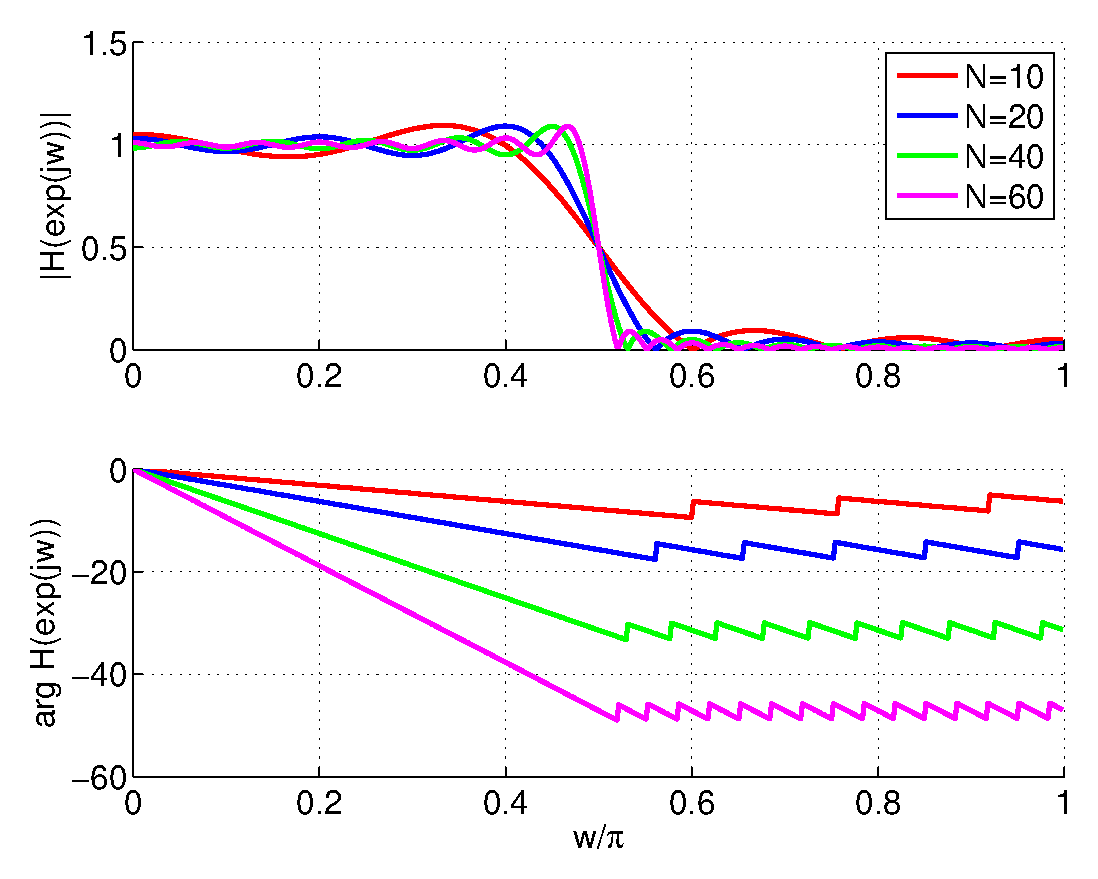
\includegraphics[width=5cm]{Figures/FIRLowTrunc.eps}
}

\visible<4->{
Desfase lineal ($-wN/2$, discont. $\pi$)

$N$ crece $\rightarrow \#_{rizos}$ crece

Tamaño rizos es constante.
}
 \end{column}
 \end{columns}
}


\end{itemize}

\end{frame}

%%%%%%%%%%%%%%%%%%%%%%%%%%

\begin{frame}
\frametitle{Diseño del filtro FIR por truncamiento II}

\begin{columns}[c]
\begin{column}{5cm}
\centering
\scriptsize

Filtro paso bajo

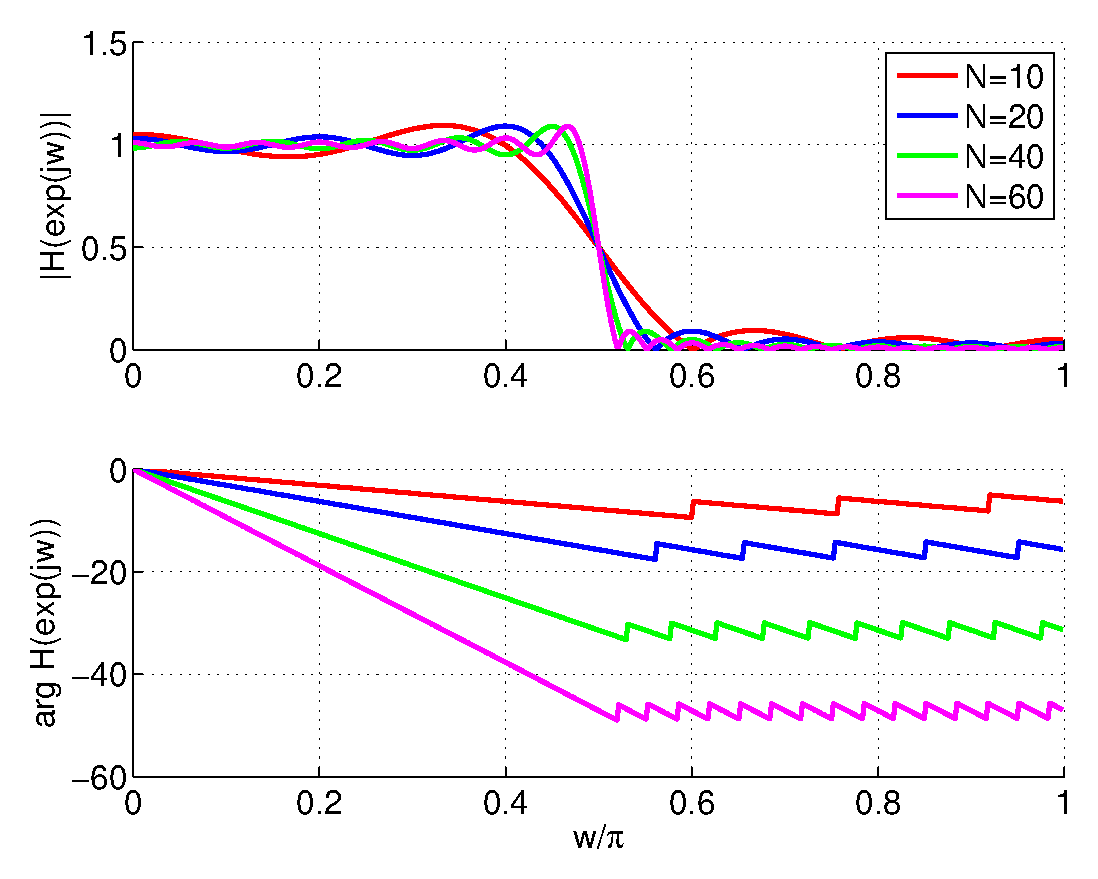
\includegraphics[width=4cm]{Figures/FIRLowTrunc.eps}

\visible<2->{

Filtro paso alto

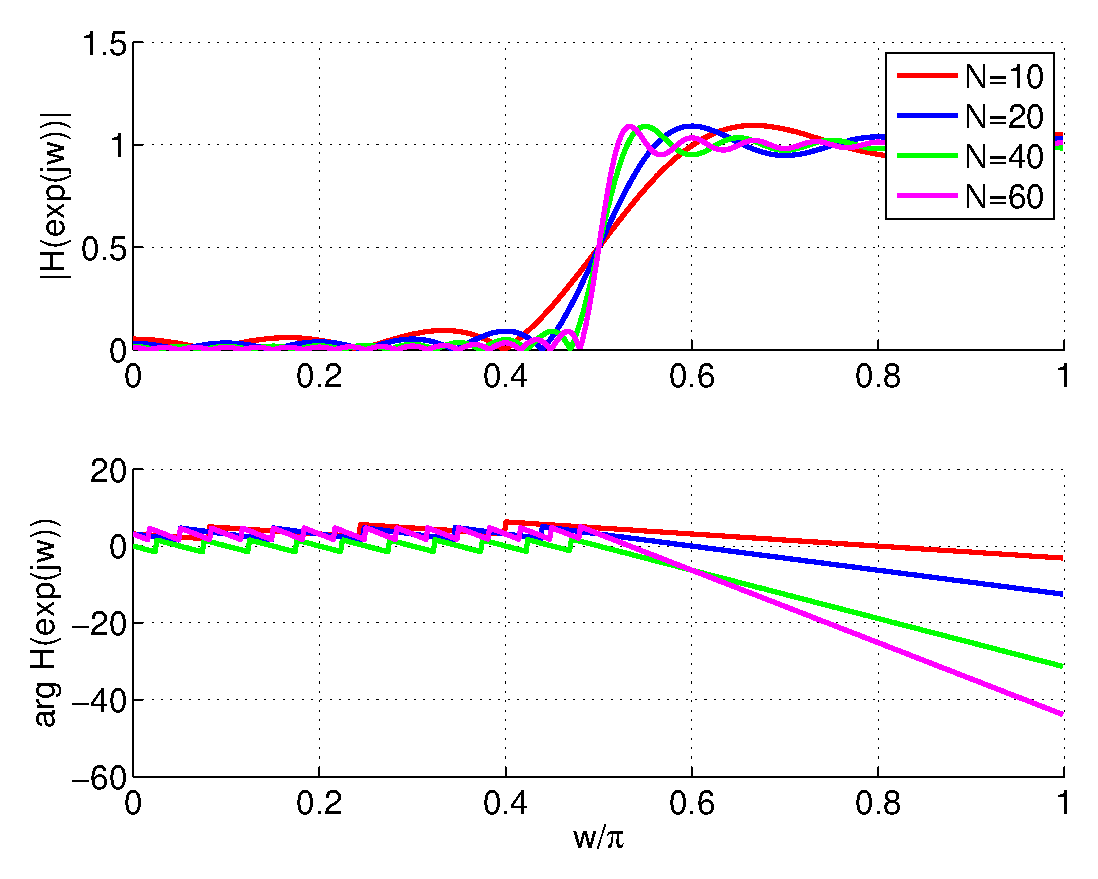
\includegraphics[width=4cm]{Figures/FIRHighTrunc.eps}

}

 \end{column}
\hspace{-0.5cm} \begin{column}{5cm}
\scriptsize

\visible<3->{
Filtro paso banda
\centering

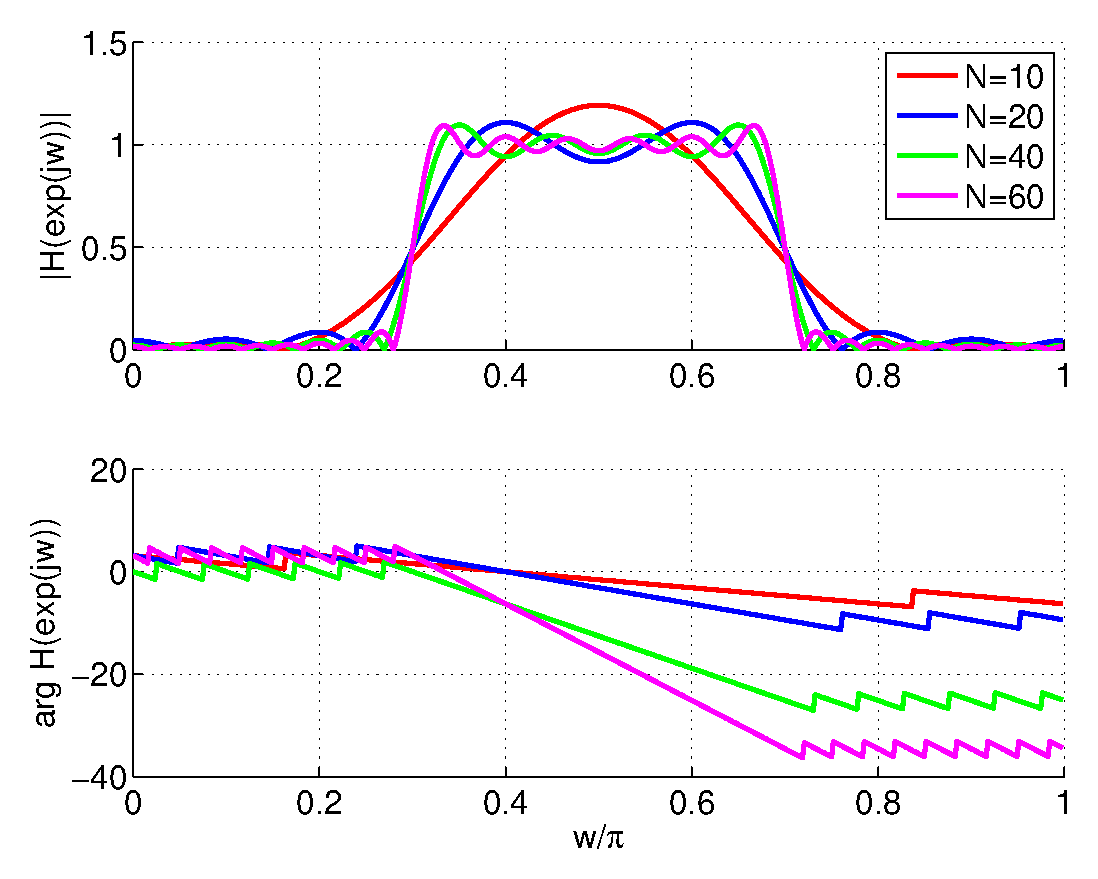
\includegraphics[width=4cm]{Figures/FIRPassTrunc.eps}

Filtro supresor banda

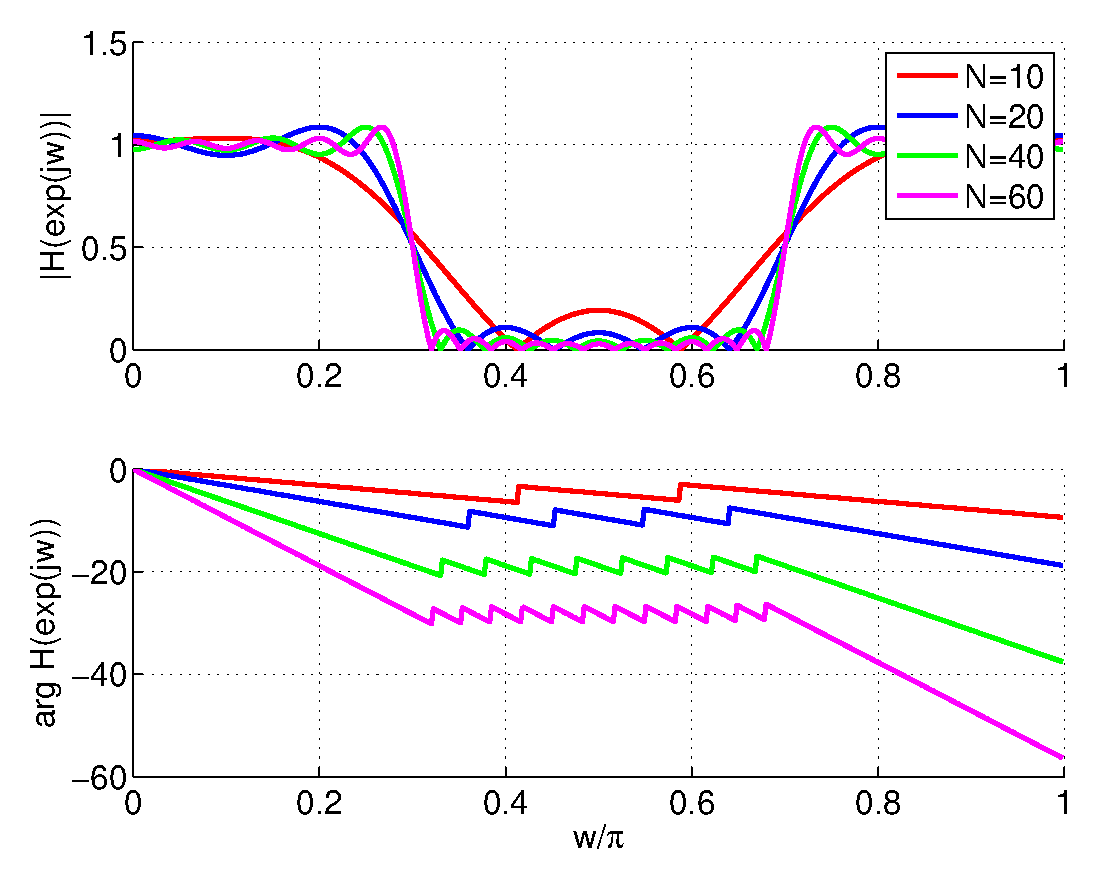
\includegraphics[width=4cm]{Figures/FIRStopTrunc.eps}

}

 \end{column}
 \end{columns}

\scriptsize

{

Desfase lineal ($-wN/2$, discont. $\pi$); tamaño rizos en el borde es constante; y según $N$ crece $\rightarrow \#_{rizos}$ crece, los rizos son más estrechos y la banda de transición decrece.
}

\end{frame}

%%%%%%%%%%%%%%%%%%%%%%%%%

\begin{frame}
\frametitle{Diseño del filtro FIR por truncamiento III}

\footnotesize

\vspace{-0.3cm}

\begin{itemize}
\item Los rizos que se producen tanto en la banda de paso como en la banda de supresión al truncar el filtro son una consecuencia directa del proceso de truncamiento. Este hecho se llama  fenómeno de Gibbs.

\visible<2->{

\item El truncamiento se puede expresar  alternativamente como el producto de la $h_d(n)$ y una ventana $v(n)$ cuadrada de longitud 2L+1: $h_t(n)\!\!=\!\!v(n)h_d(n)$.
}

\visible<3->{
\item Propiedad producto: $h_t(n)=v(n)h_d(n)$} \visible<4->{$\leftrightarrow H_t(e^{jw})=\frac{1}{2\pi}(V*H_d)_{2\pi}(e^{jw})$
}

\visible<5->{
$H_t(e^{jw})=\frac{1}{2\pi}\int_{-\pi}^\pi H_d(e^{jw})V(e^{j(w-\phi)}d\phi$
}
\vspace{-1cm}

\hspace{0.3cm}\begin{columns}[c]
\begin{column}{4cm}
\visible<6->{
$v(n)=\left \{  \begin{array}{l} 1, \:\:-L\le n \le L\\0, \:\: c.c. \end{array} \right .$

\vspace{0.1cm}

$V(e^{jw})=\frac{sen\left([2L+1]w/2\right)}{sen(w/2)}$

\vspace{0.1cm}

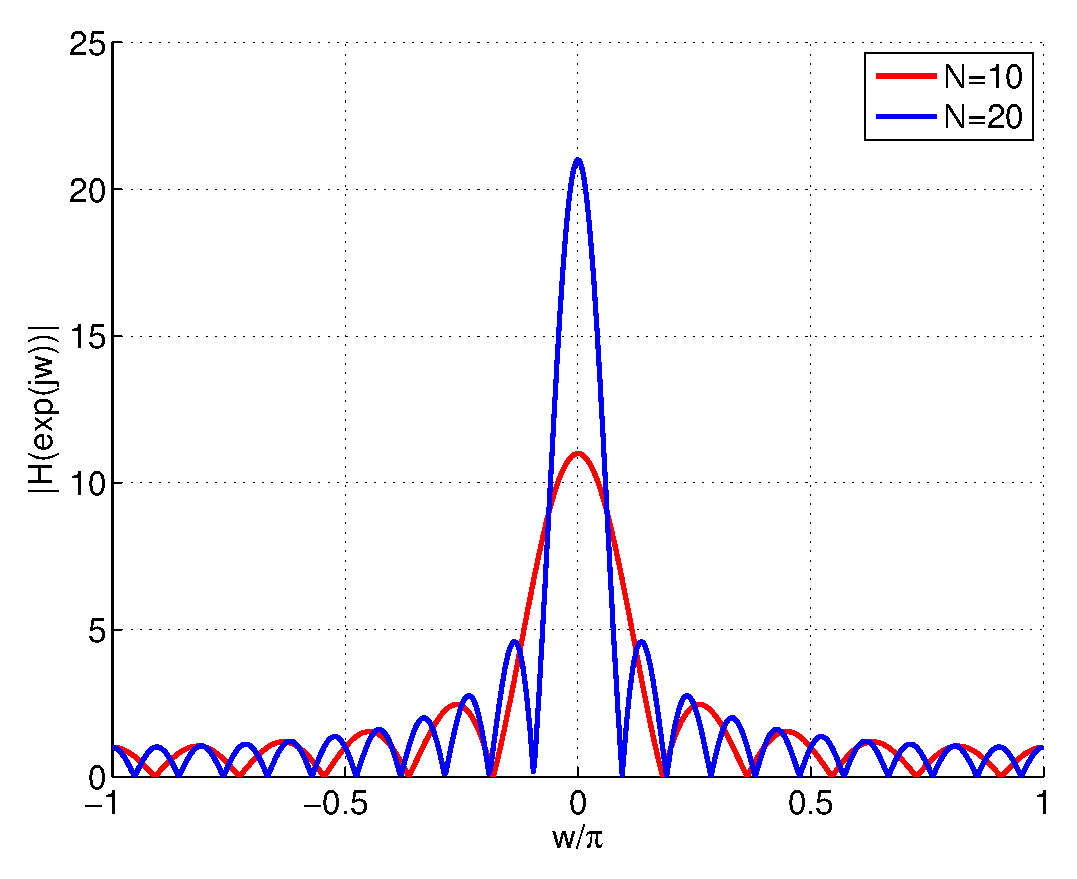
\includegraphics[width=3cm]{Figures/HwTrunc.eps}
}
\end{column}
\hspace{-2cm}\begin{column}{6.5cm}
\visible<7->{
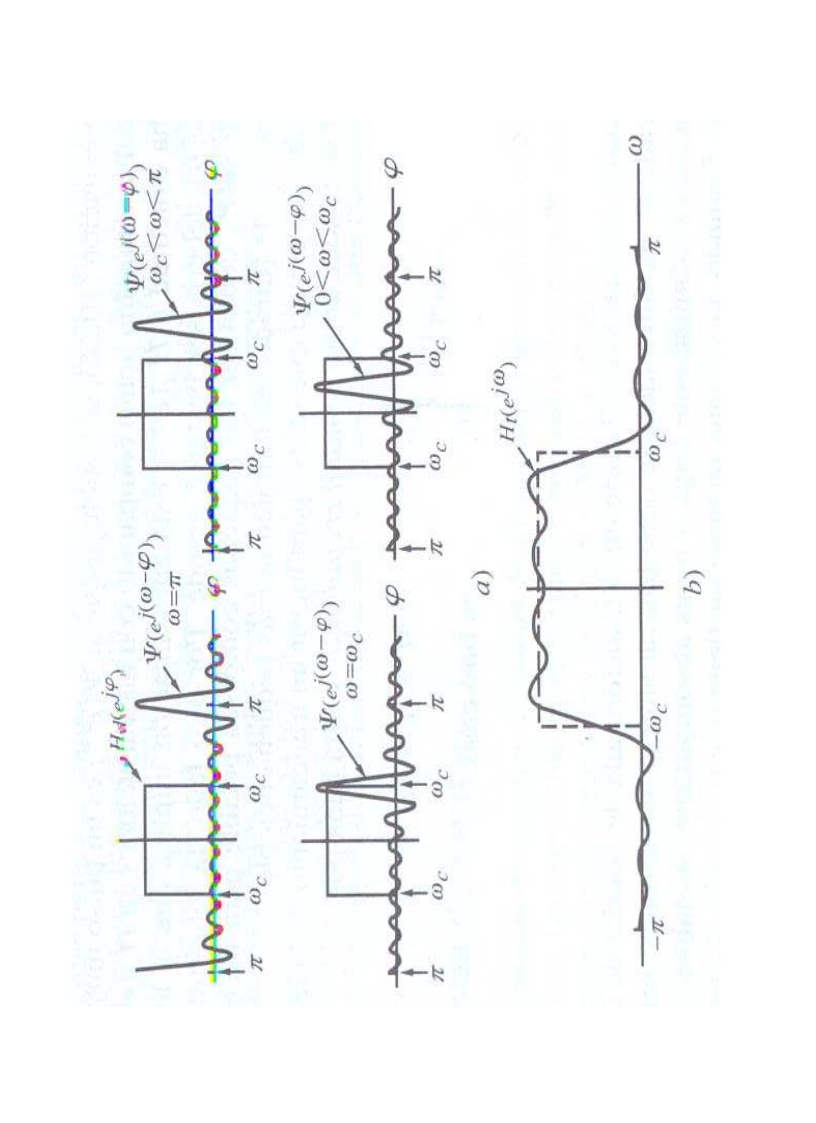
\includegraphics[trim=0cm 1cm 0cm 1cm, clip=true,angle=-90,width=6.5cm]{Figures/ConvTrunc}
}
\end{column}

\end{columns}
\visible<6->{
\vspace{-0.6cm}
\item Si $N$ crece, el lóbulo principal de $V(e^{jw})$ es más estrecho pero el area permanece cte} \visible<7->{ $\rightarrow$ los rizos de $H_t(e^{jw})$ están más cerca de la $w_c$ pero su tamaño permanece cte.
}


\end{itemize}

\end{frame}


%%%%%%%%%%%%%%%%%%%%%%%%%%



\begin{frame}
\frametitle{Diseño del filtro FIR con ventana fija I}

\vspace{-0.4cm}

\footnotesize
\begin{itemize}
\item La aparición del fenómeno de Gibbs se debe a que la ventana $v(n)$ rectangular tiene una transición abrupta.

\visible<2->{
\item Para mitigarlo, se pueden escoger ventanas con transiciones mas suaves ($-L\le n \le L$)
\begin{itemize}
\footnotesize
\item Barlett: $v(n)=1-\frac{|n|}{L+1}$
\item Hann: $v(n)=\frac{1}{2}\left [1+cos\left (\frac{2\pi n}{2L+1}\right )\right ]$
\item Hamming: $v(n)=0.54+0.46 cos \left (\frac{2\pi n}{2L+1}\right )$
\item Blackman: $v(n)=0.42+0.5 cos \left (\frac{2\pi n}{2L+1}\right )+0.08 cos \left (\frac{4\pi n}{2L+1}\right )$
\end{itemize}}
\visible<3->{
\item Las ventanas se pueden obtener con Matlab con las ordenes: \alert{\texttt{rectwin, bartlett, hann, hamming, blackman}.}
\begin{itemize}
\footnotesize
\item Ejemplo: \color{gray} \texttt{v=rectwin(2*L+1)}\color{black}
\end{itemize}}
\end{itemize}

\vspace{-0.2cm}

\begin{columns}[c]
\visible<4->{
\hspace{1cm}\begin{column}{4cm}
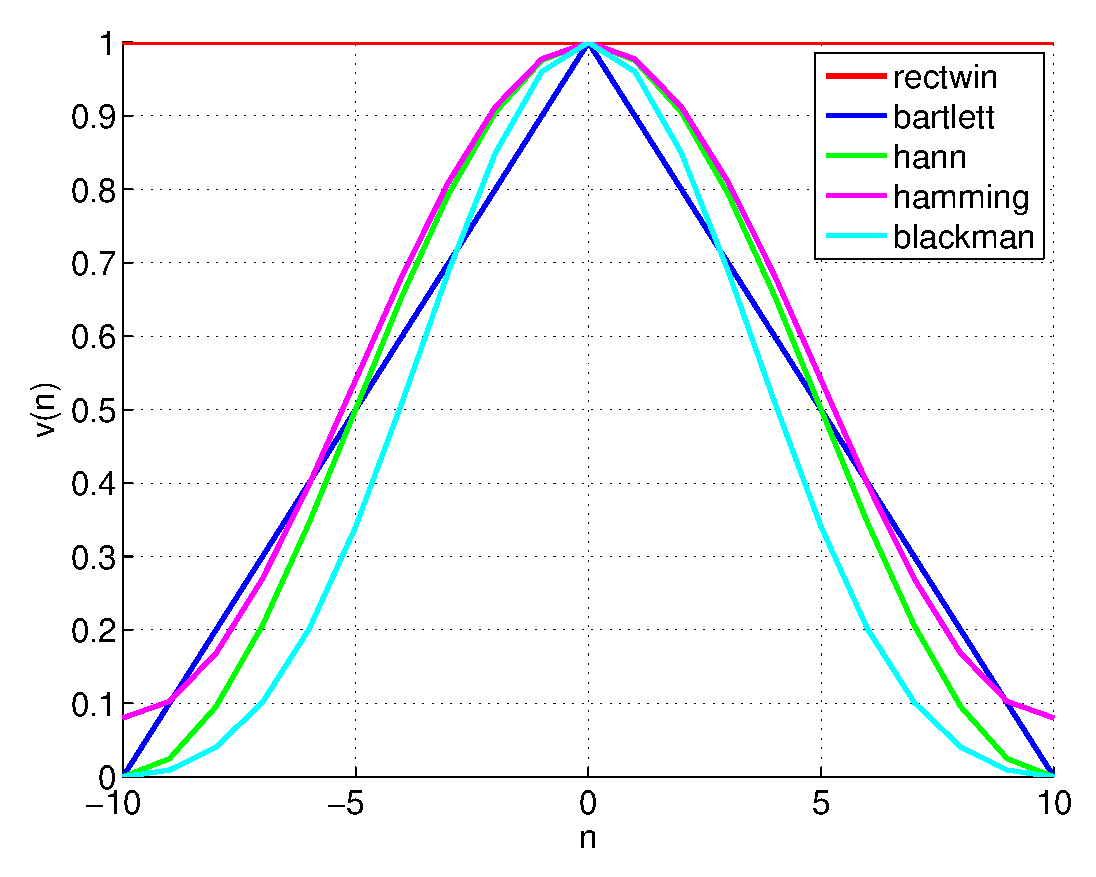
\includegraphics[trim=0cm 0cm 0cm 0cm, clip=true,angle=0,width=3.5cm]{Figures/hnWindow.eps}
\end{column}}

\visible<5->{
\hspace{-0.3cm}\begin{column}{4cm}
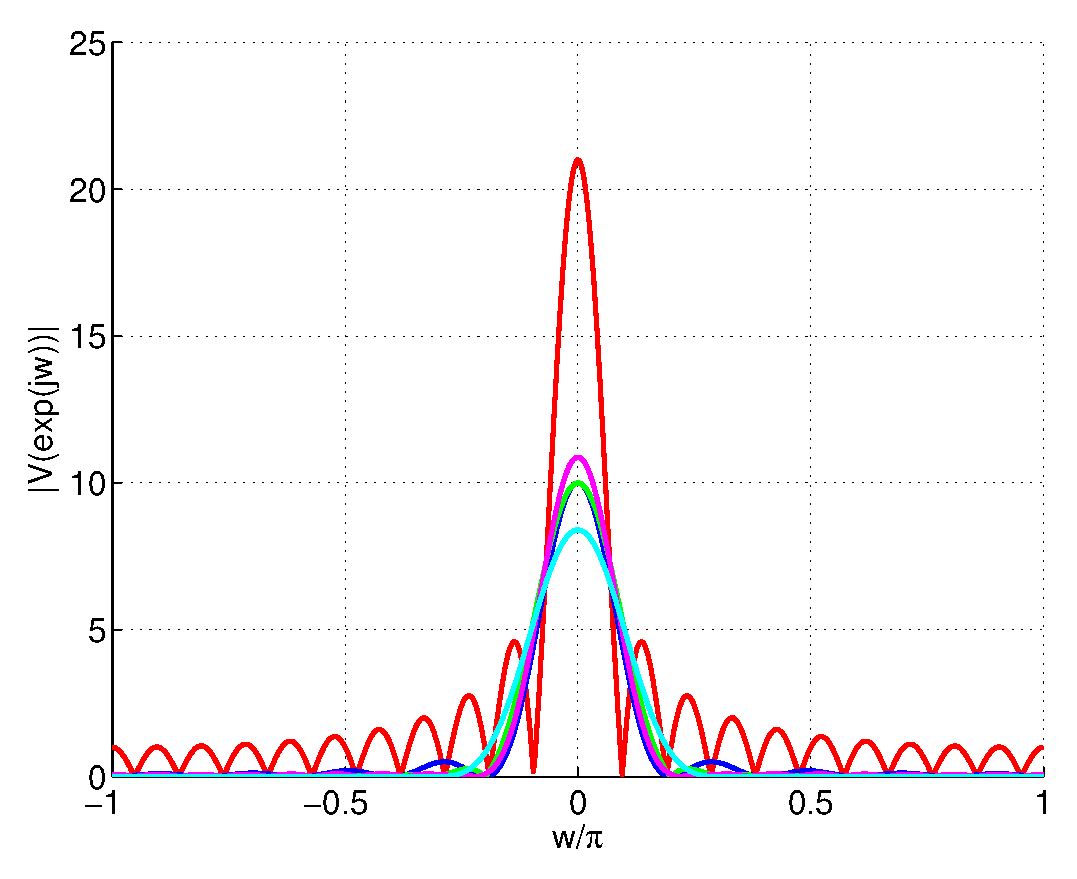
\includegraphics[trim=0cm 0cm 0cm 0cm, clip=true,angle=0,width=3.5cm]{Figures/HwWindow.eps}
\end{column}}
\hspace{-0.2cm}\begin{column}{4cm}
\scriptsize
\visible<5->{
$\Delta_{ML}$: Ancho (frecuencias) del lóbulo principal

$A_{ML}$: Nivel relativo (respecto al siguiente lóbulo) del lóbulo principal

Ambos parámetros están relacionados con el comportamiento de $H_t(n)$
}
\end{column}
\end{columns}

\end{frame}

%%%%%%%%%%%%%%%%%%%%%%%%%%%%%

\begin{frame}
\frametitle{Diseño del filtro FIR con ventana fija II}

\begin{columns}[c]
\begin{column}{7.5cm}
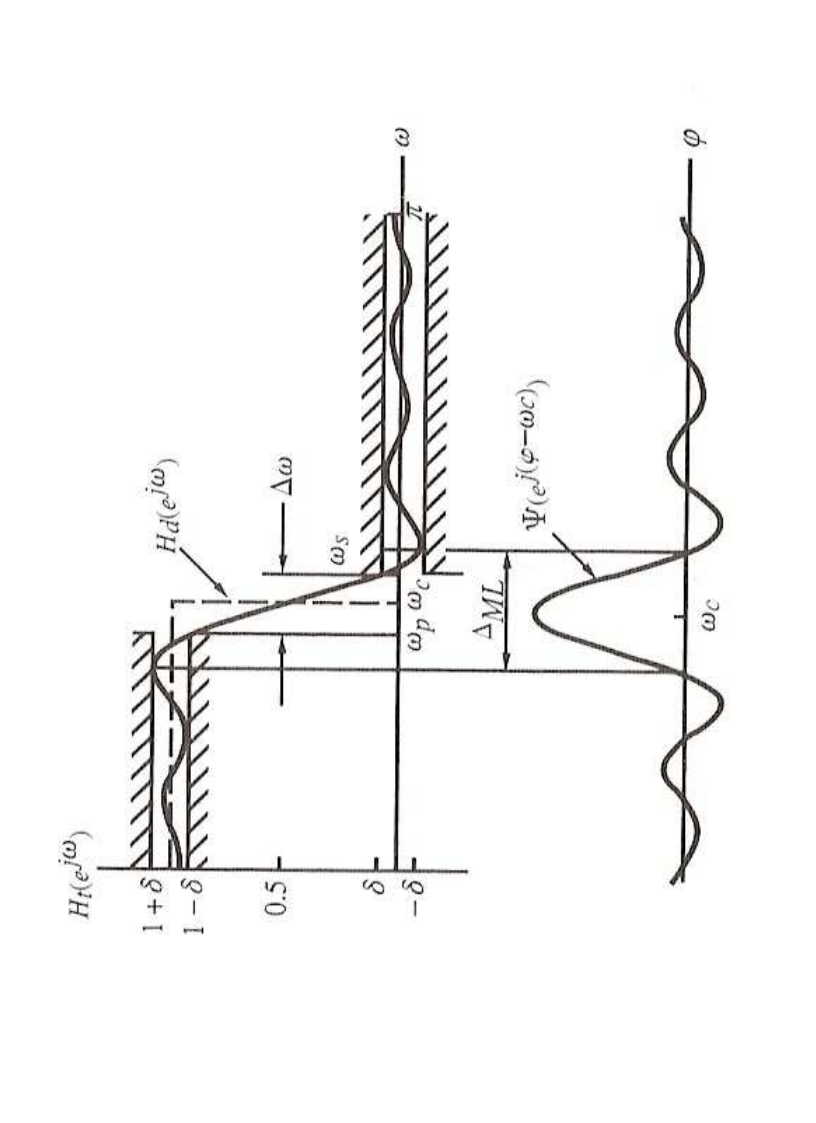
\includegraphics[trim=0cm 0cm 0cm 0cm, clip=true,angle=-90,width=7.5cm]{Figures/WindowFija1}
\end{column}

\hspace{-0.3cm}\begin{column}{4.5cm}

\begin{itemize}
\footnotesize
\item $|H(e^{jw_c})|=0.5$

\item $w_c=\frac{w_p+w_s}{2}$

\item $\Delta_w=w_s-w_p<\Delta_{ML}$

\item Tamaño del rizado $\delta$ es el mismo en ambas bandas

\item Son filtros de ventana fija, porque la atenuación (rizado) es constante.

\visible<2->{
\item M en la tabla es L.}
\end{itemize}
\end{column}

\end{columns}

\vspace{-0.5cm}
\visible<2->{
\hspace{-0.3cm}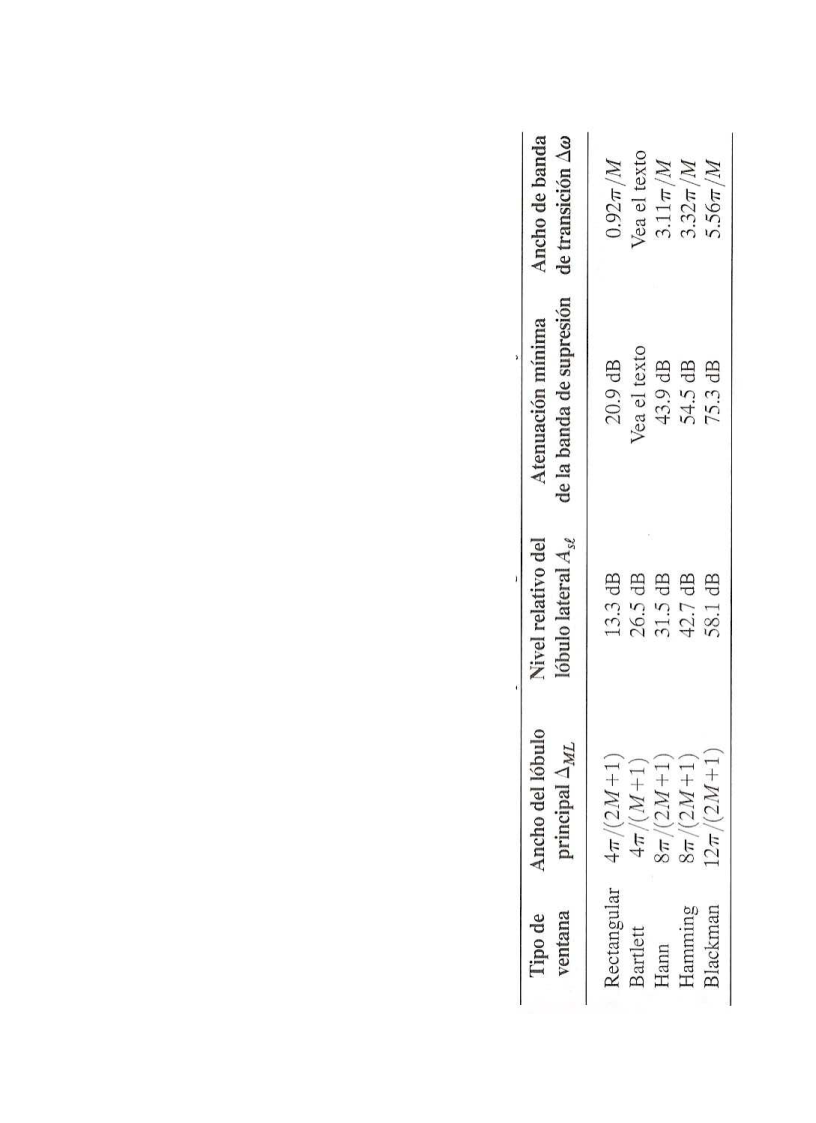
\includegraphics[trim=13cm 0cm 0cm 0cm, clip=true,angle=-90,width=12cm]{Figures/WindowFija2}}

\end{frame}

%%%%%%%%%%%%%%%%%%%%%%%%%%%%%%%%%%%%%%%%%%


\begin{frame}
\frametitle{Ejemplo FIR paso baja de ventana fija}

\footnotesize

\color{olivegreen}Diseñar un filtro paso bajo con las siguientes especificaciones:

 $w_p=0.3\pi$, $w_s=0.5\pi$, $\alpha_s=40dB$.

\color{gray}

\vspace{-0.3cm}

\hspace{-0.3cm}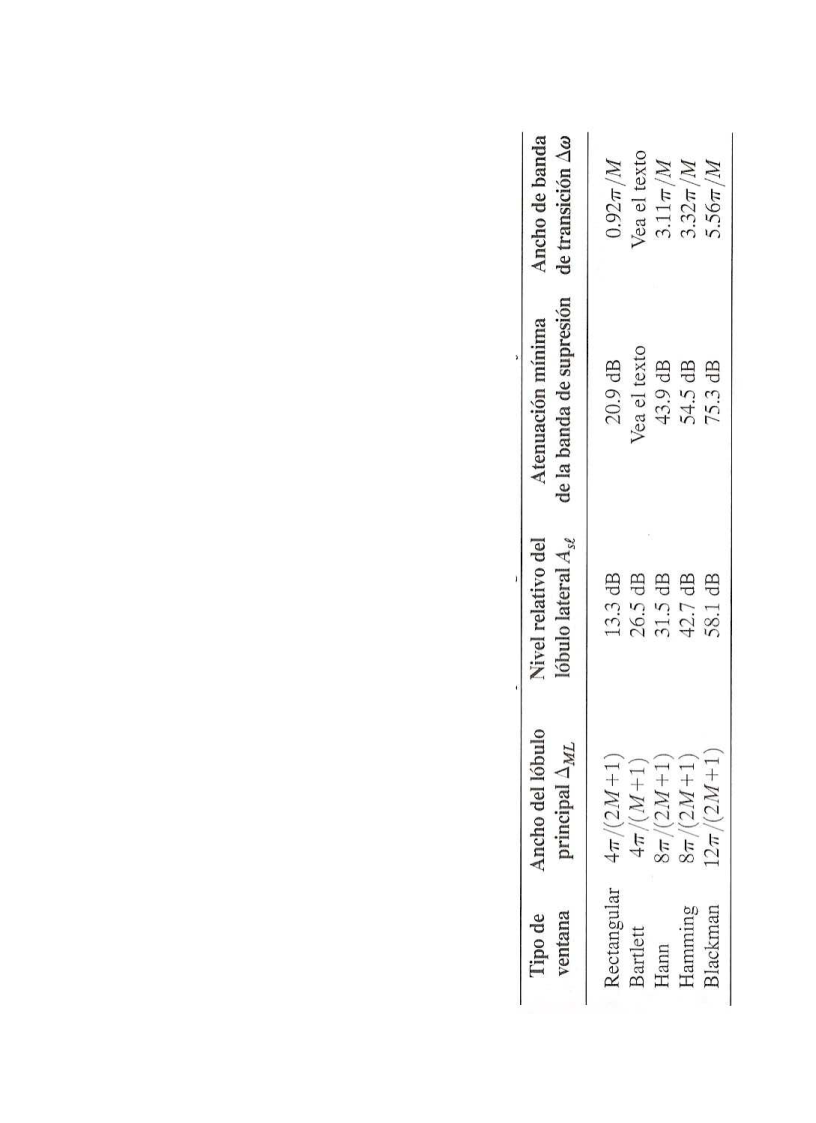
\includegraphics[trim=13.5cm 0cm 1cm 0cm, clip=true,angle=-90,width=10.5cm]{Figures/WindowFija2}

\vspace{-0.1cm}

\scriptsize

 $w_c= \frac{w_p+w_s}{2}=0.4\pi$   $\:\:\:\:\:\Delta_w=w_s-w_p=0.2\pi$

$\alpha_s=40dB$: Filtros posibles son Hann, Hamming, y Hamming



Hann: $\Delta_w=3.11\pi/L  \rightarrow L=3.11\pi/\Delta_w=15.55 \rightarrow L=16$

Hamming: $\Delta_w=3.32\pi/L  \rightarrow L=3.32\pi/\Delta_w=16.6 \rightarrow L=17$

Blackman: $\Delta_w=5.56\pi/L  \rightarrow L=5.56\pi/\Delta_w=27.8 \rightarrow L=28$

\vspace{-0.4cm}

\begin{columns}[T]
\hspace{1cm}\begin{column}{5.5cm}
\lstinputlisting{./Matlab/FIREjemplo1.m}
\end{column}
\hspace{1cm}\begin{column}{4.5cm}

\vspace{0.4cm}
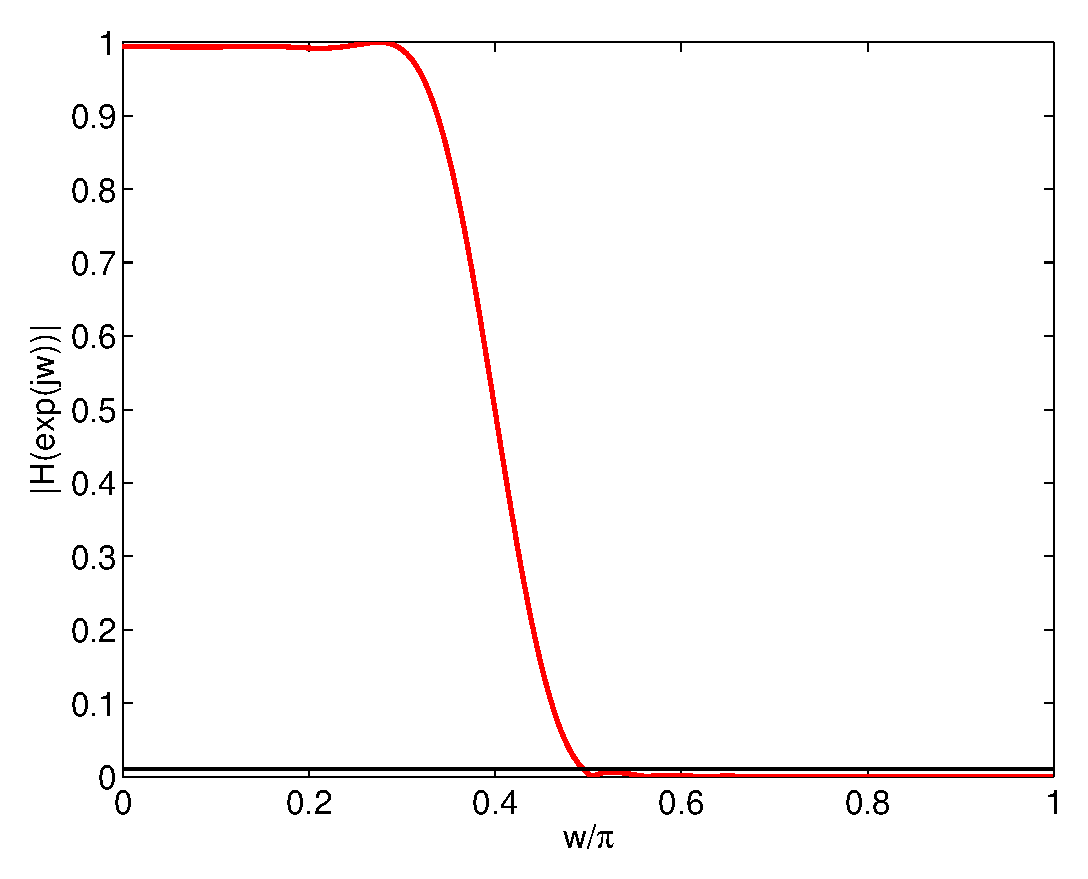
\includegraphics[trim=0cm 0cm 0cm 0cm, clip=true,angle=0,width=4cm]{Figures/FIREx1.eps}

\end{column}
\end{columns}

\end{frame}


%%%%%%%%%%%%%%%%%%%%%%%%%%%%%%%%%
\begin{frame}
\frametitle{Diseño del filtro FIR con ventana variable}
\footnotesize
\begin{itemize}
\item  El rizado de las ventanas fijas es constante
\item Para tener control sobre el valor del rizado, se  pueden usar las ventanas ajustables:
\begin{itemize}
\footnotesize
\item \alert{Dolph-Chebyshev}: \texttt{ v=chebwin(2*L+1,Asl)}
$v(n)=\frac{1}{2L+1}\left[ \frac{1}{\gamma}+\sum_{k=1}^L T_{2N}\left( \beta cos (\frac{k\pi}{2L+1})\right) cos (\frac{2nk\pi}{2L+1})\right]$

$\gamma=\frac{\mathrm{amplitud \:\: lobulo  \:\: lateral}}{\mathrm{amplitud \:\: lobulo  \:\: principal}}$,  $\:\:\:\beta=cosh\left(\frac{1}{2L}acosh(1/\gamma)\right)$

$T_l(x)=\left \{ \begin{array}{l}cos(l \cdot acos(x)), \:\: |x|<1\\cosh(l \cdot acosh(x)), \:\: |x|<1 \end{array}\right .$
 \alert{$\:\:2L=\frac{2.056\alpha_s-16.4}{2.285\Delta w}$}


\vspace{0.2cm}


\item \alert{Kaiser}: \texttt{ v=kaiser(2*L+1,beta)}

\vspace{0.1cm}

$v(n)=\frac{I_o\left(\beta \sqrt{1-(n/L)^2}\right)}{I_o\left(\beta\right)}$

\vspace{0.1cm}

$I_o(u)=1+\sum_{r=1}^\infty \left(\frac{(u/2)^r}{r!}\right).$

$\beta=\left\{\begin{array}{l}0.11102(\alpha_s-8.7), \:\: \alpha_s>50\\0.5482(\alpha_s-21)^{0.4}+0.07886(\alpha_s-21), \:\: 50 \le \alpha_s \le 21\\0, c.c.\end{array} \right .$


\alert{$2L=\frac{\alpha_s-8}{2.285\Delta w}$}

\end{itemize}

\end{itemize}

\end{frame}

%%%%%%%%%%%%%%%%%%%%%%%%%%%%%%%%

\begin{frame}
\frametitle{Ejemplo FIR paso baja de ventana Dolph-Chebyshev}

\footnotesize

\color{olivegreen}Diseñar un filtro paso bajo con las siguientes especificaciones:

 $w_p=0.3\pi$, $w_s=0.5\pi$, $\alpha_s=40dB$.

\color{gray}

 $w_c= \frac{w_p+w_s}{2}=0.4\pi$   $\:\:\:\:\:\Delta_w=w_s-w_p=0.2\pi$

$2L=\frac{2.056\alpha_s-16.4}{2.285\Delta w}  \rightarrow L=22.92  \rightarrow L=23$


\begin{columns}[T]
\hspace{1cm}\begin{column}{5.5cm}
\lstinputlisting{./Matlab/FIREjemplo2.m}
\end{column}
\hspace{1cm}\begin{column}{4.5cm}

\vspace{0.4cm}
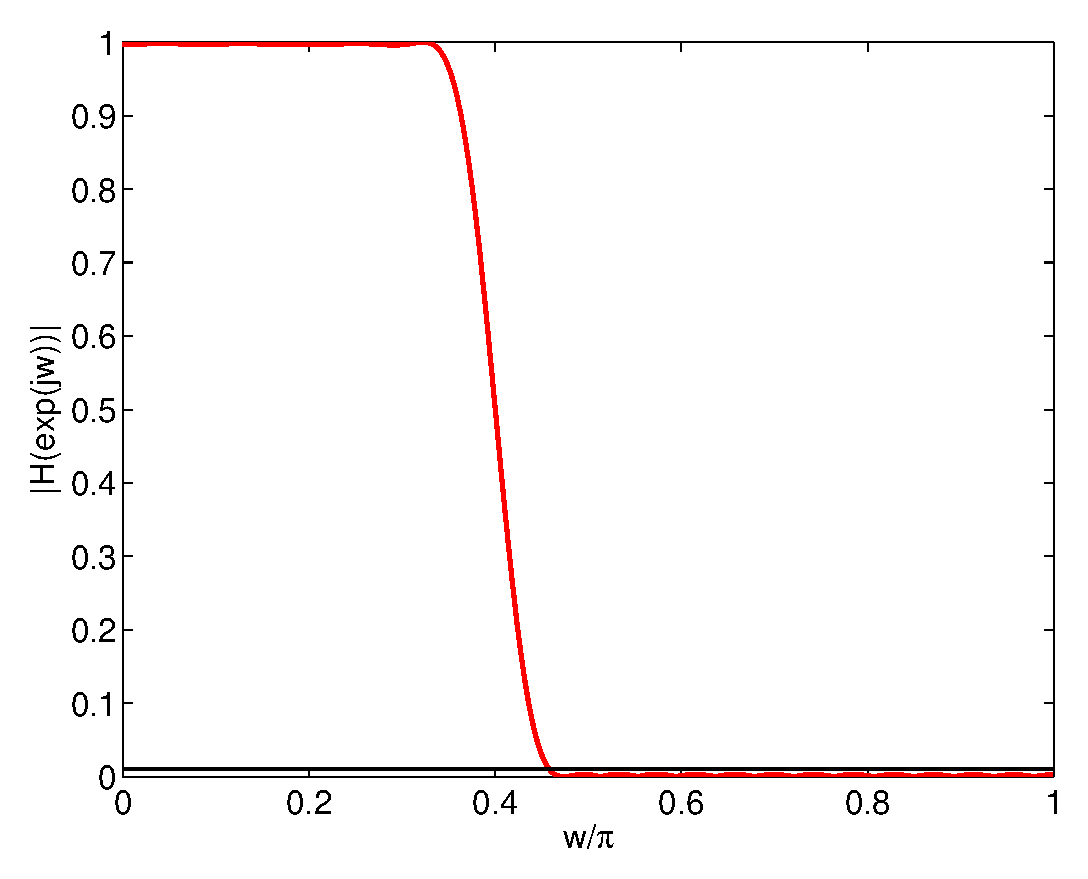
\includegraphics[trim=0cm 0cm 0cm 0cm, clip=true,angle=0,width=4.2cm]{Figures/FIREx2.eps}

\end{column}
\end{columns}

\end{frame}


\begin{frame}
\frametitle{Ejemplo FIR paso baja de ventana Kaiser}

\footnotesize

\color{olivegreen}Diseñar un filtro paso bajo con las siguientes especificaciones:

 $w_p=0.3\pi$, $w_s=0.5\pi$, $\alpha_s=40dB$.

\color{gray}

 $w_c= \frac{w_p+w_s}{2}=0.4\pi$   $\:\:\:\:\:\Delta_w=w_s-w_p=0.2\pi$

$2L=\frac{\alpha_s-8}{2.285\Delta w}  \rightarrow L=11.14  \rightarrow L=12$

$\beta=0.5482(\alpha_s-21)^{0.4}+0.07886(\alpha_s-21)=3.2784$

\begin{columns}[T]
\hspace{1cm}\begin{column}{5.5cm}
\lstinputlisting{./Matlab/FIREjemplo3.m}
\end{column}
\hspace{1cm}\begin{column}{4.5cm}

\vspace{0.4cm}
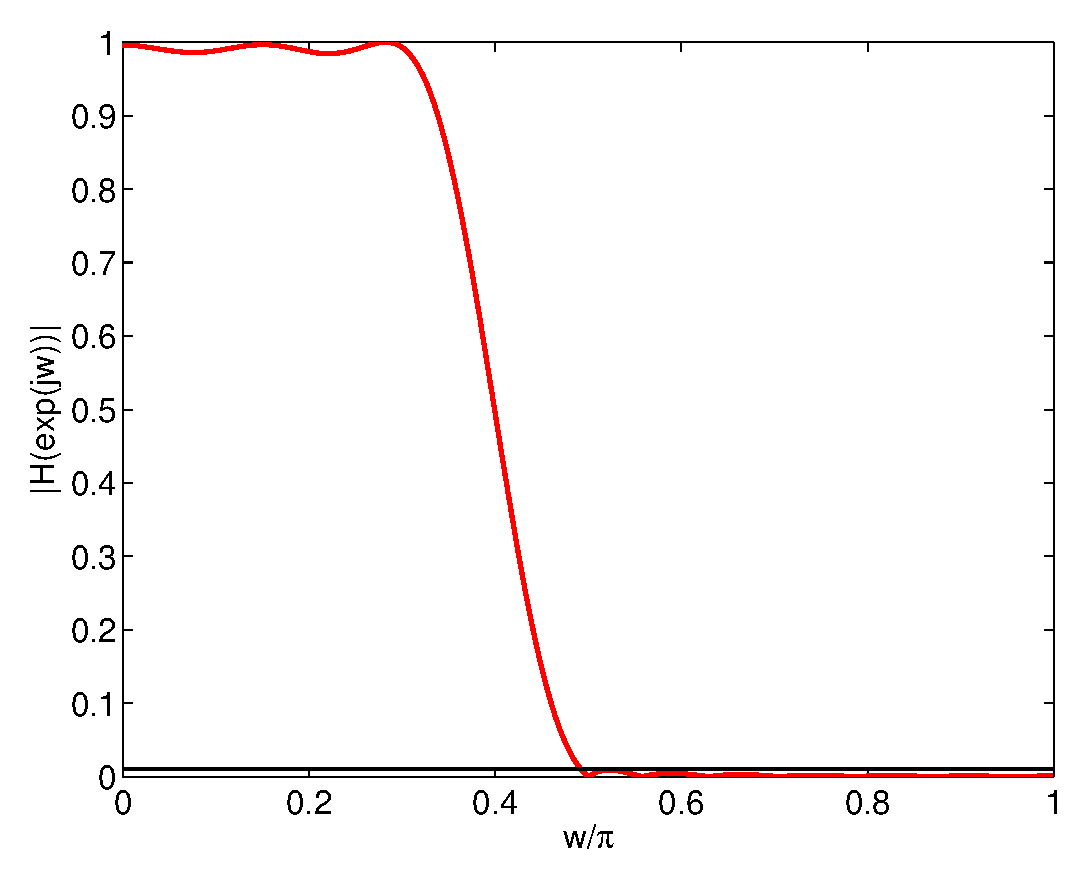
\includegraphics[trim=0cm 0cm 0cm 0cm, clip=true,angle=0,width=4.2cm]{Figures/FIREx3.eps}

\end{column}
\end{columns}

\end{frame}

%%%%%%%%%%%%%%%%%%%%%%%

\begin{frame}
\frametitle{Diseño de filtros avanzados con Matlab}
\footnotesize
\begin{itemize}
\item Adicionalmente, Matlab facilita los cálculos con ordenes adicionales:
\begin{itemize}
\footnotesize
\item Ordenes relacionadas con la ventana de Kaiser:

\texttt{[N,wc,beta,type]=kaiserord([wp,ws],[A1,A2],[dp,ds])}

\texttt{window=kaiser(N+1,beta);}

\texttt{h=fir1(N,wc,type,window);}

\item Ordenes para el diseño de filtros  multinivel:


\texttt{ws=[w0,w1,...,wM];}

\texttt{A=[A0,A1,...AM];}

\texttt{h=fir2(N,ws,A,window)};



\end{itemize}
\end{itemize}
\end{frame}




\begin{frame}
\frametitle{Ejemplo FIR paso alto de ventana Kaiser}

\footnotesize

\color{olivegreen}Diseñar un filtro paso alto con las siguientes especificaciones:

 $w_p=0.55\pi$, $w_s=0.4\pi$, $\delta_s=0.01$.

\color{gray}

\begin{columns}[T]
\begin{column}{6.5cm}
\lstinputlisting{./Matlab/FIREjemplo4.m}
\end{column}
\hspace{-0.5cm}\begin{column}{4.5cm}

\vspace{0.4cm}
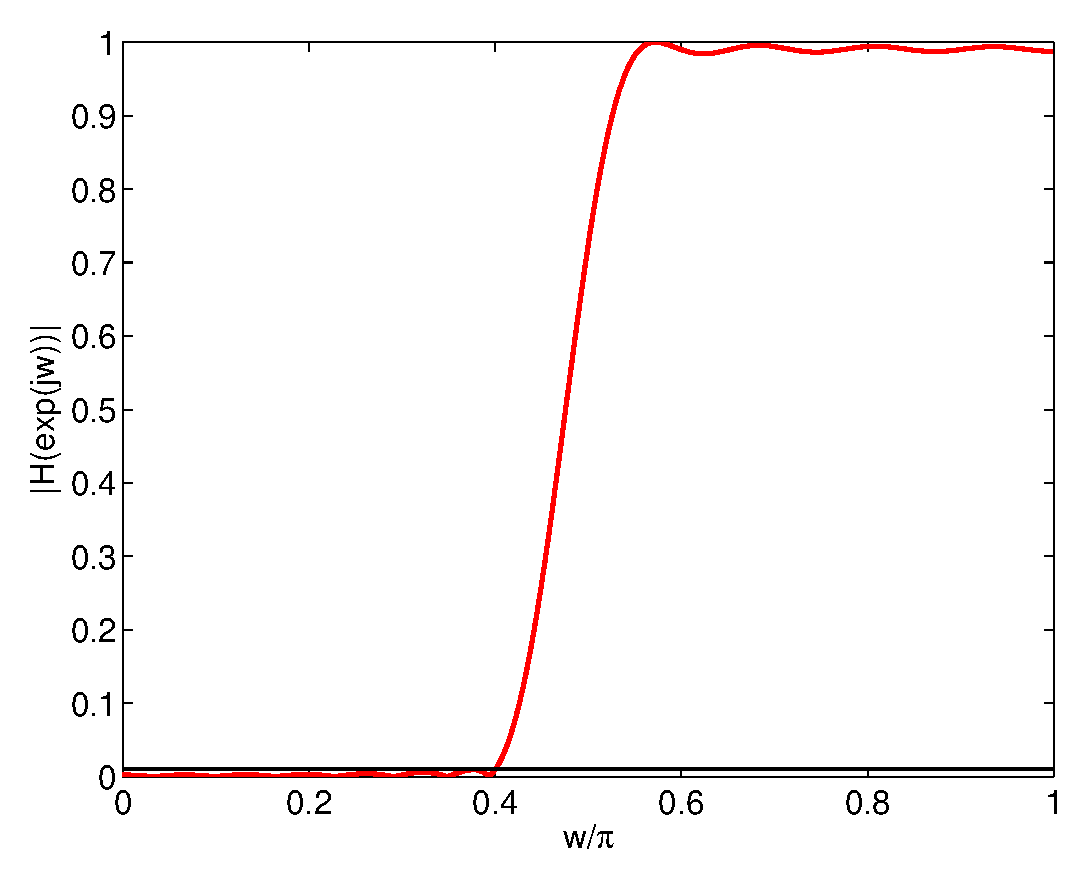
\includegraphics[trim=0cm 0cm 0cm 0cm, clip=true,angle=0,width=4.2cm]{Figures/FIREx4.eps}

\end{column}
\end{columns}

\end{frame}

%%%%%%%%%%%%%%%%%%%%%%%%%%%%%%%%%%%%%%%%%%%%%%%


\begin{frame}
\frametitle{Ejemplo FIR multibanda}

\footnotesize

\color{olivegreen}Diseñar un filtro multibanda con ventana de Hamming con las siguientes especificaciones:

w=[0,0.28,0.3,0.5,0.52,1];

A=[0.3,0.3,1.0,1.0,0.7,0.7];


\color{gray}

\begin{columns}[T]
\begin{column}{6.5cm}
\lstinputlisting{./Matlab/FIREjemplo5.m}
\end{column}
\hspace{-0.5cm}\begin{column}{4.5cm}

\vspace{0.4cm}
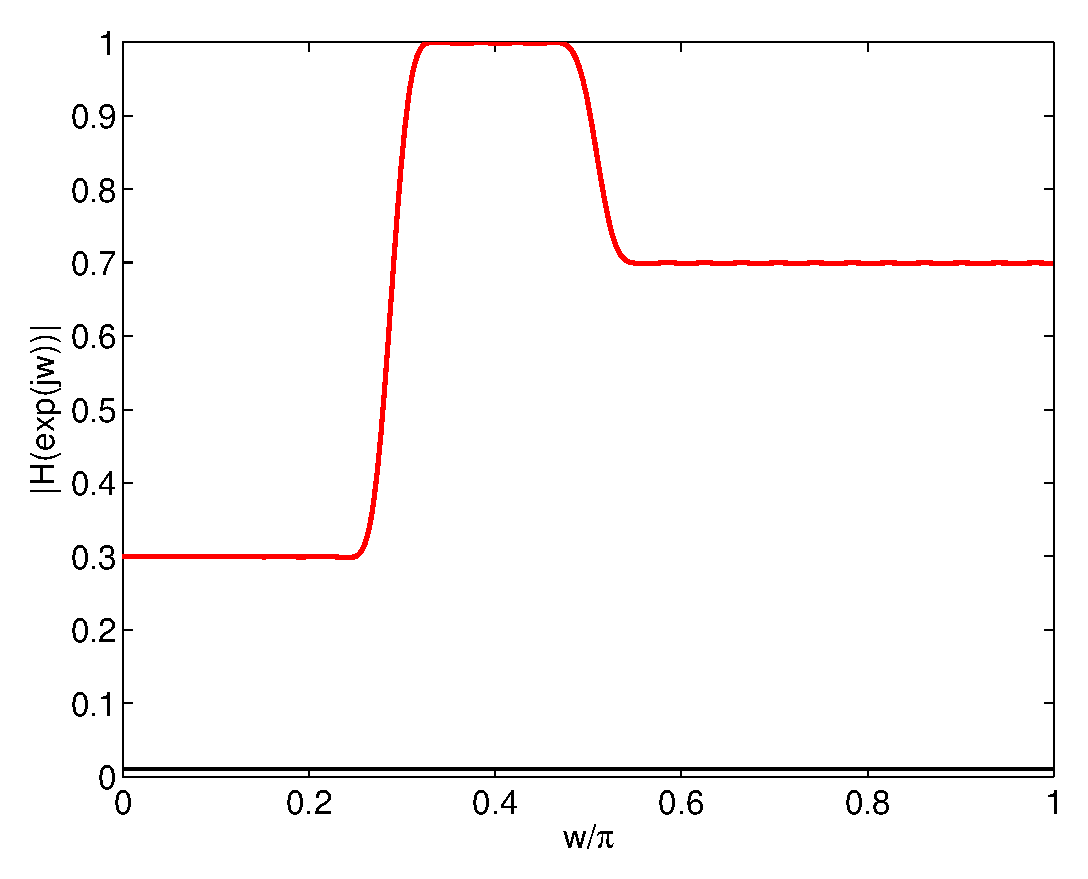
\includegraphics[trim=0cm 0cm 0cm 0cm, clip=true,angle=0,width=4.2cm]{Figures/FIREx5.eps}

\end{column}
\end{columns}

\end{frame}


\begin{frame}
\frametitle{Métodos alternativos cálculo de N}

\vspace{-0.4cm}

\footnotesize
\begin{itemize}
\item Existen expresiones  adicionales para estimar el orden (N+1) del filtro:

\begin{itemize}

\vspace{-0.1cm}

\footnotesize

\item Kaiser: $\displaystyle N \approx \frac{-20 log_{10}\left( \sqrt{\delta_p \delta_s}\right)-13}{14.6(w_s-w_p)/(2\pi)}$

%\vspace{0.1cm}

\item Bellanger: $\displaystyle  N \approx - \frac{-2 log_{10}( 10 \delta_p \delta_s)}{3(w_s-w_p)/(2\pi)}$

%\vspace{0.1cm}

\item Hermann: $\displaystyle  N \approx  \frac{D_\infty(\delta_p,\delta_s)-F_\infty(\delta_p,\delta_s)\left [(w_s-w_p)/(2\pi)\right ]^2}{(w_s-w_p)/(2\pi)}$

{\scriptsize
$D_\infty(\delta_p,\delta_s)=\left [a_1 \left (log_{10}(\delta_p)\right )^2+ a_2 log_{10}(\delta_p)+a_3\right ]log_{10}(\delta_s)-$

\hspace{1.8cm}$-\left [a_4 \left (log_{10}(\delta_p)\right )^2+ a_5 log_{10}(\delta_p)+a_6\right ]$

\vspace{0.1cm}

$F_\infty(\delta_p,\delta_s)=11.01217 + 0.51244 \left ( log_{10}(\delta_p)-log_{10}(\delta_s)\right )$

\vspace{0.1cm}


\hspace{-0.2cm}$\begin{array}{lll}a_1=0.005309 &a_2=0.07114 & a_3=-0.4761 \\ a_4=0.00266 &a_5=0.5941&a_6=0.4278\end{array}$

}


\end{itemize}
\vspace{-0.3cm}
\scriptsize{
\item Si $\delta_p < \delta_s$ hay que cambiar la una por la otra en la fórmula de Hermann
\item Para valores elevados de los rizos es mejor usar la ecuación de Hermann
\item Las formulas estiman N.  Si el filtro no cumple los requisitos, incrementar  N.
\item En los filtros paso/supresor banda, hay dos bandas de transición. Usar la banda más estrecha.}
\end{itemize}

\vspace{-0.4cm}

\rule{12cm}{0.4pt}

\scriptsize

Las formulas están en función de los rizos: $\alpha_p=-20 log_10(1-\delta_p)$, $\alpha_s=-20 log_10(\delta_s)$

\end{frame}


\subsection{Comparativa IIR vs. FIR}

\begin{frame}
\frametitle{Filtros IIR vs. filtros FIR}

{\footnotesize
\hspace{0.5cm}\alert{IIR:} $\displaystyle H(z)=\frac{p_0+p_1 z^{-1}+ \dots +p_M z^{-M}}{d_0+d_1 z^{-1}+ \dots +d_N z^{-N}}$
\hspace{0.5cm}\alert{FIR:} $H(z)=h_0+\dots h_N z^{-N}$}
\begin{itemize}
\small
\item En los filtros FIR solo es posible colocar ceros (atenuar), mientras que en los filtos IIR se puede colocar ceros (atenuar) y polos (amplificar)
\item Para dos filtros del mismo orden N, el número de operaciones de un filtro FIR es menor que el número de operaciones del filtro IIR. 
\item Para dos filtros con las mismas prestaciones (características de la respuesta en frecuencia), el orden del filtro IIR suele ser menor que el orden del filtro FIR
\item Para diseñar filtros de fase (desfase) lineal se puede:
\begin{itemize}
\item Si el filtro es FIR, usar las técnicas de TF con ventana o hacer que las $h(n)$ cumplan una relaciones especiales. 
\item Si el filtro es IIR, introducir un filtro paso todas que modifique el desfase introducido por el filtro IIR. La introducción del filtro paso todas reduce el ahorro computacional debido a la reducción del orden del filtro.
\end{itemize}

\end{itemize}
\end{frame}

% 
\section{Técnicas adicionales de diseño}



%%%%%%%%%%%%%%%%%%%%%%%%%%%%%%%%%%%

\begin{frame}
\frametitle{Filtros Paso Todas}

\vspace{-0.2cm}



\begin{itemize}
\footnotesize
\item Un filtro paso todas cumple que : $|H(e^{jw})|=1 \:\: \forall w$

\visible<2->{

\item Un filtro IIR con coeficientes reales y causal de la forma

$H(z)=\pm \frac{d_M + d_{M-1}z^{-1}+\dots+ z^{-M}}{1+d_1z^{-1}+\dots+ d_M z^{-M}}=\pm \frac{z^{-M}D_M(z^{-1})}{D_M(z)}$

\hspace{4cm}$D_M(z)=1+d_1 z^{-1}+\dots + d_M z^{-M}$


}

\visible<3->{

\item Es por construcción un filtro paso todas:

$|H(e^{jw})|^2\!=\!H(e^{jw})H(e^{-jw})\!=\!H(z)H(z^{-1})|_{z=e^{jw}}\!=\!(\pm)^2 \frac{z^{-M}D_M(z^{-1})}{D_M(z)} \frac{z^{M}D_M(z)}{D_M(z^{-1})}=1$

}

\visible<4->{

\item $z_{POLO}=re^{j\theta}  \leftrightarrow z_{CERO}=\frac{1}{r}e^{j\theta}$

\item Si el filtro es estable $\rightarrow$ tiene sus polos (raíces de $D_M(z)$) dentro del círculo unidad y sus ceros (raíces de $D_M(z^{-1})$) fuera del círculo unidad. Los polos y los ceros se encuentran enfrentados con una simetría especular respecto al círculo.

}

\visible<5->{

\item Como no atenúan ninguna frecuencia, son útiles para modificar el desfase introducido por otros filtros. 

}

\visible<6->{

\item El desfase total introducido por el filtro paso todas H(z) entre las frecuencias $w\in[0 ,\pi]$ es de $M\pi$. 

}
\end{itemize}
\end{frame}

\begin{frame}
\frametitle{Ejemplo Filtros Paso Todas}
\footnotesize

\color{olivegreen} Comprobar el comportamiento del filtro $H(z)= \frac{z^{-M}D_M(z^{-1})}{D_M(z)}$, con 
$D_M(z)=1+0.4 z^{-1}+0.18z^{-2}-0.2z^{-3}$

\color{gray}

\begin{columns}[c]
\begin{column}{4cm}
\lstinputlisting{./Matlab/EjPasoTodos.m}
\end{column}
\begin{column}{5cm}
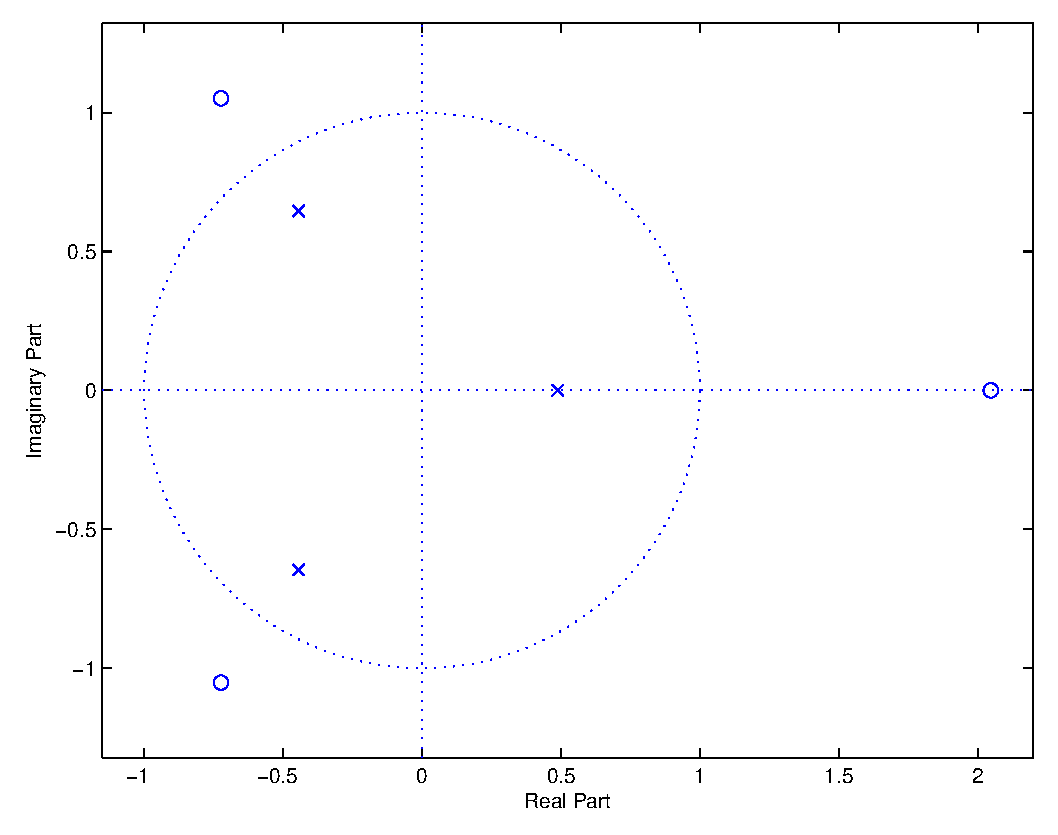
\includegraphics[width=4cm]{./Figures/EjPasoTodo1.eps}

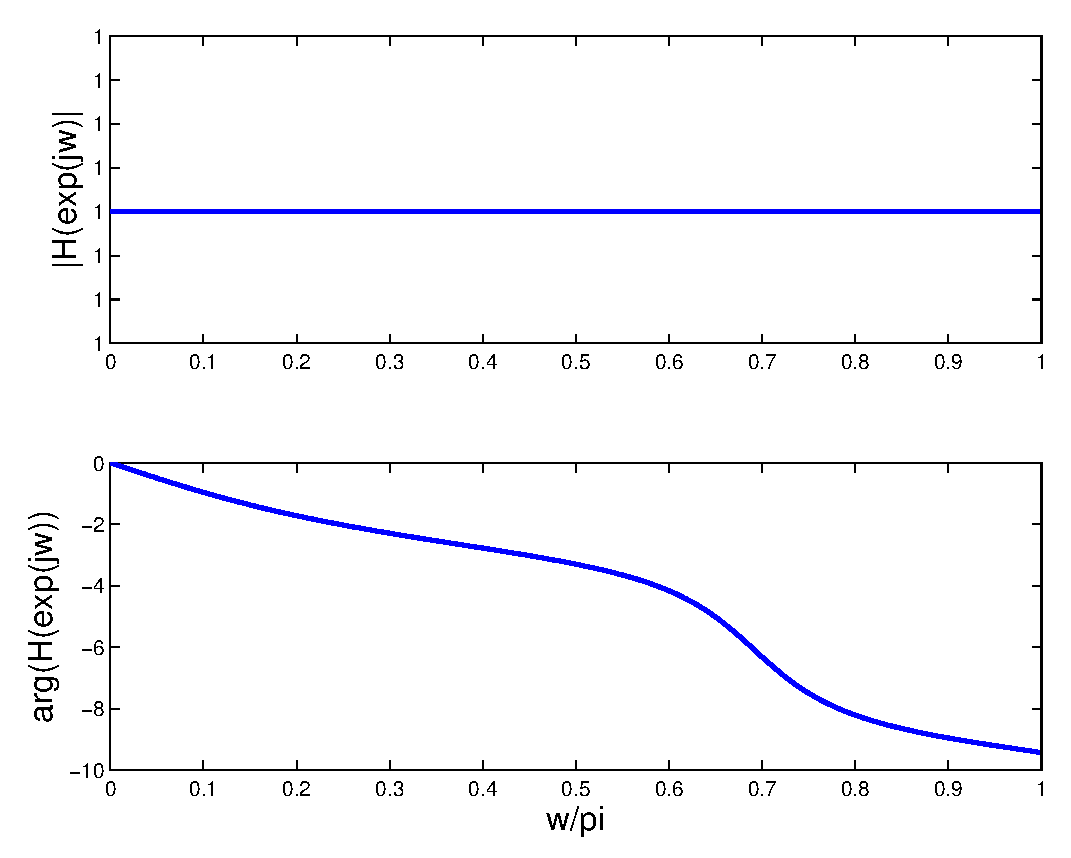
\includegraphics[width=4cm]{./Figures/EjPasoTodo2.eps}
\end{column}
\end{columns}


\end{frame}




%%%%%%%%%%%%%%%%%%%%%%%%%%%%%%%%%%%

\begin{frame}
\frametitle{Filtros de fase 0 - I }

\vspace{-0.2cm}



\begin{itemize}
\footnotesize
\item Un filtro de de fase 0 es aquel que tiene una $H(e^{jw})$ real y no negativa.

\visible<2->{

\item Esto implica que no modifica la fase de la señal de entrada en la banda de paso.
}

\visible<3->{

\item Se puede implementar como  $H(z)=F(z)F(z^{-1})$, donde  F(z) es un sistema que no tiene polos sobre el círculo unidad. 

}

\visible<4->{

\item Por construcción es un filtro de fase 0:

$H(e^{jw})\!=H(z=e^{jw})=F(e^{jw})F(e^{-jw})=|F(e^{jw})|^2$, que es un número positivo real.

}

\visible<5->{

\item Si z es un polo (o cero) del sistema su inversa también lo es. Por lo tanto se colocan con una simetría especular respecto al circulo unidad. 
}

\visible<6->{


\item Este hecho hace que el sistema sea inestable, y que por lo tanto no se pueda aplicar directamente a una señal. 
}

\visible<7->{

\item Sin embargo, si se puede aplicar a una señal de longitud finita:

\begin{columns}[T]
\begin{column}{4cm}

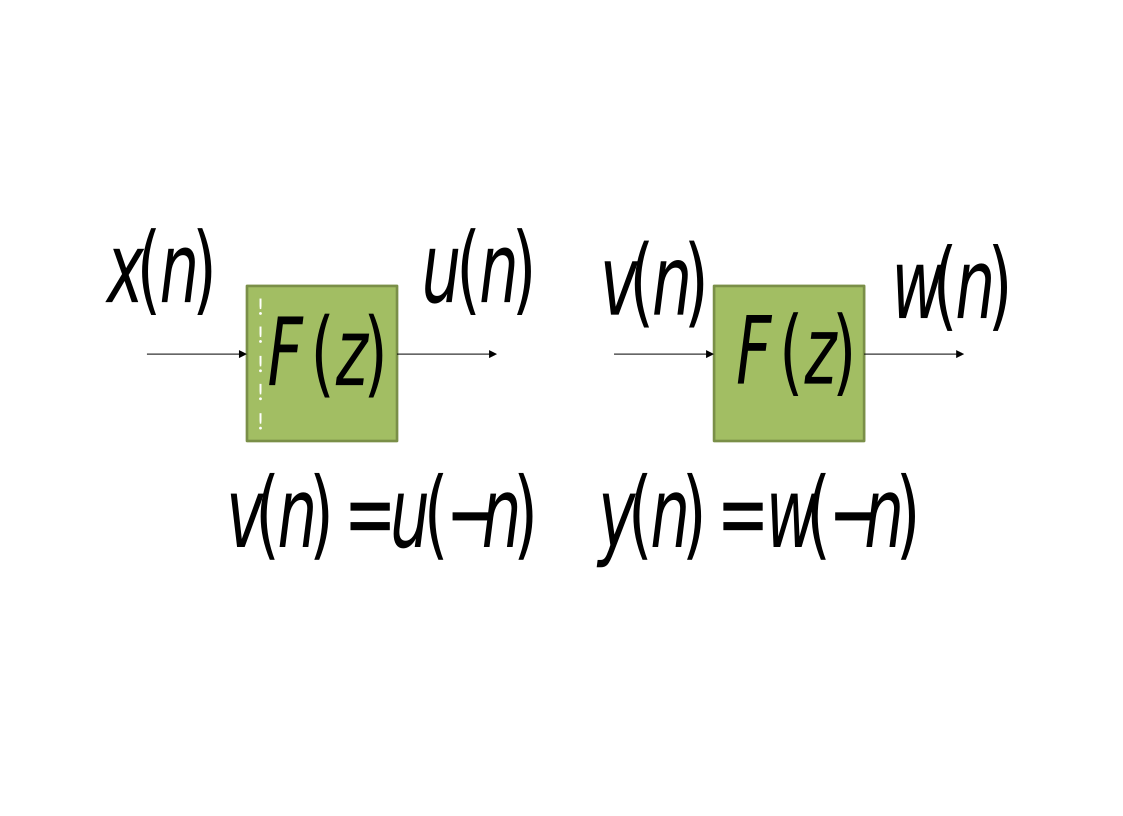
\includegraphics[trim=4cm 1cm 4cm 1cm,width=4cm]{Figures/FiltroFase0}
\end{column}
\begin{column}{4cm}

$Y(e^{jw})=W^*(e^{jw})=F^*(e^{jw})V^*(e^{jw})=F^*(e^{jw})U(e^{jw})=F^*(e^{jw})F(e^{jw})X(e^{jw})=|F(e^{jw})|^2X(e^{jw})$
\end{column}
\end{columns}
}



\visible<8->{
\item La orden de Matlab \color{blue}\texttt{y=filtfilt(Fnumz,Fdenz,x)}\color{black} permite realizar el filtrado con el procedimiento anteriormente escrito.
}


\end{itemize}
\end{frame}

\begin{frame}
\frametitle{Ejemplo Filtro Fase 0 - II}
\footnotesize

\begin{itemize}

\item Implementación a través de la $F(z)$: $H(z)=F(z)F(z^{-1})$

\hspace{4.8cm} $H(e^{jw})=|F(e^{jw})|^2$

\visible<2->{

\item El hecho de que en $H(z)$ aparezca un polo y su inversa, hace que el numerador y el denominador sean productos de polinomios   $B(z)=\sum_{l=0}^N b_l(z^l+z^{-l})$

\color{gray}

Ejemplo: $(z-a)(z^{-1}-a)=(1-az-az^{-1}+a^2)=(1+a^2)+a(z^1+z^{-1})$

\color{black}
}

\visible<3->{


\item Una forma habitual de diseñar este tipo de filtros es definir la $H(e^{jw})$ deseada, y obtener a continuación la F(z) aprovechando la propiedad de que la localización de los ceros y polos con simetría especular hace que en la H(z) aparezcan productos de polinomios $B(z)=\sum_{l=0}^N b_l(z^l+z^{-l})$, y que esto a su vez implica que en la respuesta en frecuencia tendremos términos del tipo $B(e^{jw})=\sum_{l=0}^N b_l(e^{jwl}+e^{-jwl})=b_0+\sum_{l=0}^N 2b_lcos(wl)$


\item A continuación veremos con un ejemplo la forma de proceder.
}

\end{itemize}
\end{frame}

\begin{frame}
\frametitle{Ejemplo Filtro Fase 0}
\footnotesize

\color{olivegreen} Calcular la F(z) de un filtro de fase 0 con  $H(e^{jw})=\frac{4(1.09+0.6cos(w))(1.16-0,8cos(w))}{(1.04-0.4cos(w))(1.25+cos(w))}$




\color{gray}

\vspace{0.2cm}

$H(e^{jw})=|F(e^{jw})|^2=\frac{4(1.09+0.3(e^{jw}+e^{-jw}))(1.16-0,4(e^{jw}+e^{-jw}))}{(1.04-0.2(e^{jw}+e^{-jw}))(1.25+0.5(e^{jw}+e^{-jw}))}$

\vspace{0.2cm}

$F(z)F(z^{-1})=\frac{4(1.09+0.3(z+z^{-1}))(1.16-0,4(z+z^{-1}))}{(1.04-0.2(z+z^{-1}))(1.25+0.5(z+z^{-1}))}=$

\vspace{0.2cm}

$F(z)F(z^{-1})=\frac{4(1+0.3z)(1+0.3z^{-1})(1-0.4z)(1-0.4z^{-1})}{(1-0.2z)(1-0.2z^{-1})(1+0.5z)(1+0.5z^{-1})}$

\vspace{0.2cm}

$F(z)=\frac{2(1+0.3z)(1-0.4z)}{(1-0.2z)(1+0.5z)}$


\end{frame}





%%%%%%%%%%%%%%%%%%%%%%%%%%%%%%%%%%%

\begin{frame}
\frametitle{Filtros FIR con $h(n)$ real y $H(e^{jw})$ de fase lineal I}

\vspace{-0.2cm}



\begin{itemize}
\footnotesize
\item Un filtro FIR con respuesta en frecuencia de fase lineal cumple que:
\begin{itemize}
\footnotesize
\item $H(e^{jw})=\sum_{n=0}^N h(n)e^{-jwn}=e^{j(\alpha w + \beta)} \hat H(e^{jw})$, con $\hat H(e^{jw})$ respuesta fase cero (respuesta en amplitud ($\pm$) vs. desfase).
\end{itemize}

\visible<2->{

\item Un filtro FIR con $h(n)$ real cumple que:

\begin{itemize}
\footnotesize
\item {$H^*(e^{jw})=H(e^{-jw})$}  \visible<3->{ $\rightarrow$ \alert{$\hat H(e^{jw})e^{j(\alpha w+\beta)}=\hat H(e^{-jw})e^{-j(\alpha(-w)+\beta)}$  (*)}}

\item El módulo de la respuesta en frecuencia es una función par: $|H(e^{jw})|=|H(e^{-jw})|$  \visible<4->{$\rightarrow$ \alert{ $\hat H(e^{jw})= \pm \hat H(e^{-jw})$}}

\end{itemize}

}

\visible<5->{\item Si  \alert{$\hat H(e^{jw})=+ \hat H(e^{-jw})$}}  \visible<10->{\alert{$\rightarrow h(n)=h(N-n)$} y \alert{$H(e^{jw})=\pm e^{-j\frac{N}{2}w}\hat H(e^{jw})$}}

\color{gray}
{\scriptsize
\visible<6->{

(*) $\rightarrow e^{j(\alpha w+\beta)}\!=\!e^{j(\alpha w-\beta)} \rightarrow e^{j\beta}\!=\!e^{-j\beta} $ $\rightarrow \beta\!=\!k\pi$}

\visible<7->{

$H(e^{jw})=e^{j(\alpha w + \beta)} \hat H(e^{jw}) \rightarrow  \hat H(e^{jw})=\pm e^{-j\alpha w} H(e^{jw})=\pm\sum_{n=0}^{N} h(n) e^{-jw(n+\alpha)} $}

\visible<8->{

\alert{$\hat H(e^{jw})=\pm\sum_{n=0}^{N} h(n) e^{-jw(n+\alpha)}$  }}

\visible<9->{
$\hat H(e^{-jw})=\pm\sum_{l=0}^{N} h(l) e^{jw(l+\alpha)}=\pm\sum_{n=N}^{0} h(N-n) e^{jw(N-n+\alpha)}$
}

\visible<10->{
$\sum_{n=0}^{N} h(n) e^{-jw(n+\alpha)}\!=\!\sum_{n=N}^{0} h(N-n) e^{jw(N-n+\alpha)}  \rightarrow \alpha\!=\!-N/2\:$ y $\:h(n)\!=\!h(N\!-\!n)$}
}

\color{black}
\visible<5->{\item Si \alert{$\hat H(e^{jw})=- \hat H(e^{-jw})$}} \visible<11->{\alert{$\rightarrow h(n)=-h(N-n)$} y \alert{$H(e^{jw})= e^{-j(\frac{N}{2}w \mp \frac{\pi}{2})}\hat H(e^{jw})$}}


\color{gray}

\visible<11->{

{\scriptsize
(*) $\rightarrow e^{j(\alpha w+\beta)}\!=\!-e^{j(\alpha w-\beta)} \rightarrow e^{j\beta}\!=-\!e^{-j\beta} $ $\rightarrow \beta=\frac{\pi}{2} \:\:$ o $\:\:\beta=\frac{3\pi}{2}$ 

$H(e^{jw})=e^{j(\alpha w + \beta)} \hat H(e^{jw}) \rightarrow  \hat H(e^{jw})=\mp  j e^{-j\alpha w} H(e^{jw})=\mp j\sum_{n=0}^{N} h(n) e^{-jw(n+\alpha)} $

\alert{$\hat H(e^{jw})=\mp j \sum_{n=0}^{N} h(n) e^{-jw(n+\alpha)}$  }

$\hat H(e^{-jw})=\mp j \sum_{l=0}^{N} h(l) e^{jw(l+\alpha)}=\mp j \sum_{n=N}^{0} h(N-n) e^{jw(N-n+\alpha)}$

$\sum_{n=0}^{N} h(n) e^{-jw(n+\alpha)}\!=\!-\!\sum_{n=0}^{N} h(N-n) e^{jw(N-n+\alpha)}  \rightarrow \alpha\!=\!-N/2$ y $h(n)\!=\!-h(N\!-\!n)$
}
}
\end{itemize}
\end{frame}

%%%%%%%%%%%%

\begin{frame}
\frametitle{Filtros FIR con $h(n)$ real y $H(e^{jw})$ de fase lineal II}
\footnotesize
\begin{itemize}
\item Además de las dos posibilidades de la respuesta de fase cero ($\hat H(e^{jw})=\pm \hat H(e^{-jw})$), N puede ser par o impar. Este hecho hace que existan cuatro tipos de filtro FIR de fase lineal:

\item Si  \alert{$\hat H(e^{jw})=+ \hat H(e^{-jw})$}  \alert{$\rightarrow h(n)=h(N-n)$}, \alert{$H(e^{jw})=\pm e^{-j\frac{N}{2}w}\hat H(e^{jw})$} y

\hspace{3.5cm} \alert{$\hat H(e^{jw})=\pm\sum_{n=0}^{N} h(n) e^{-jw(n-N/2)}$  }

\begin{itemize}
\footnotesize

\visible<2->{

\item Tipo 1: $h(n)=h(N-n)$ con $0\le n \le N$ y N par:

\vspace{0.1cm}
\hspace{1.05cm}$\hat H(e^{jw})=h(N/2)+2\sum_{n=1}^{N/2}h(\frac{N}{2}-n)cos(wn)$

}

\vspace{0.2cm}
\visible<3->{

\item Tipo 2: $h(n)=h(N-n)$ con $0\le n \le N$ y N impar:

\vspace{0.1cm}
\hspace{1.05cm}$\hat H(e^{jw})=2\sum_{n=1}^{(N+1)/2}h(\frac{N+1}{2}-n)cos(w(n-1/2))$
}
\end{itemize}

\item Si \alert{$\hat H(e^{jw})=- \hat H(e^{-jw})$} \alert{$\rightarrow h(n)=-h(N-n)$}, \alert{$H(e^{jw})= e^{-j(\frac{N}{2}w \mp \frac{\pi}{2})}\hat H(e^{jw})$} y

\hspace{3.5cm} \alert{$\hat H(e^{jw})=\mp j \sum_{n=0}^{N} h(n) e^{-jw(n-N/2)}$  }


\begin{itemize}
\footnotesize

\visible<4->{

\item Tipo 3: $h(n)=-h(N-n)$ con $0\le n \le N$ y N par:

\vspace{0.1cm}
\hspace{1.05cm}$\hat H(e^{jw})=h(N/2)+2\sum_{n=1}^{N/2}h(\frac{N}{2}-n)sen(wn)$
}

\vspace{0.2cm}

\visible<5->{

\item Tipo 4: $h(n)=-h(N-n)$ con $0\le n \le N$ y N impar:

\vspace{0.1cm}
\hspace{1.05cm}$\hat H(e^{jw})=2\sum_{n=1}^{(N+1)/2}h(\frac{N+1}{2}-n)sen(w(n-1/2))$
}
\end{itemize}
\end{itemize}

\end{frame}

%%%%%%%%%%

\begin{frame}
\frametitle{Filtros FIR con $h(n)$ real y $H(e^{jw})$ de fase lineal III}
\footnotesize
\begin{itemize}
\item Localización de los ceros:
\begin{itemize}
\footnotesize
\item $h(n)$ es real tiene las raíces (ceros) reales o complejas conjugadas

\vspace{0.1cm}

\item Si los filtros son FIR de fase lineal:

\begin{itemize}
\footnotesize
\item $h(n)=h(N-n)$

\vspace{0.1cm}

$H(z)\!=\!\sum_{n=0}^N h(n)z^{-n}\!=\!\sum_{n=0}^N h(N\!-\!n)z^{-n}\!=\!\sum_{m=0}^N h(m)z^{-N\!+\!m}\!=$

\vspace{0.1cm}

\hspace{0.7cm}$=\!z^{-N}H(z^{-1})$


\vspace{0.1cm}

\item $h(n)=-h(N-n)$

\vspace{0.1cm}

$H(z)\!=\!\sum_{n=0}^N \!h(n)z^{-n}\!=\!\!-\!\sum_{n=0}^N \!h(N\!-\!n)z^{-n}\!=\!\!-\!\sum_{m=0}^N \!h(m)z^{-N\!+\!m}\!=$

\vspace{0.1cm}

\hspace{0.7cm}$=\!-z^{-N}H(z^{-1})$

\end{itemize}
\end{itemize}
\item Como $z=re^{j\theta}$ y $z^{-1}=\frac{1}{r}e^{-j\theta}$, los ceros de los FIR de fase lineal representan una simetría especular respecto al círculo unidad.

\item Los cuatro tipos de filtros se diferencian en el número de ceros que hay en +1 y -1.
\begin{itemize}
\scriptsize
\item \alert{Tipo 1 (N par): Un número par o ningún cero en +1 y -1.}
\item \alert{Tipo 2 (N impar): Un número par o ningún cero en +1 y un número impar en -1.}
\item \alert{Tipo 3 (N par): Un número impar en +1 y -1.}
\item \alert{Tipo 4 (N impar): Un número impar +1 y un número par o ninguno en -1.}

\end{itemize}


\end{itemize}

\end{frame}

%%%%%%%%%%%%%%%%%%%%%%%

\begin{frame}
\frametitle{Filtros FIR con $h(n)$ real y $H(e^{jw})$ de fase lineal IV}

\footnotesize

Resumen de las características:

\begin{itemize}

\item Como $z=re^{j\theta}$ y $z^{-1}=\frac{1}{r}e^{-j\theta}$, los ceros de los FIR de fase lineal representan una simetría especular respecto al círculo unidad.

\item $h(n)=h(N-n)$ con $0\le n \le N$,  $\:\:H(e^{jw})=\pm e^{-j\frac{N}{2}w}\hat H(e^{jw})$


\begin{itemize}
\footnotesize
\item Tipo 1: N par, y un número par o ningún cero en +1 y -1

\vspace{0.1cm}

\hspace{1.05cm}$\hat H(e^{jw})=h(N/2)+2\sum_{n=1}^{N/2}h(\frac{N}{2}-n)cos(wn)$



\vspace{0.1cm}

\item Tipo 2: N impar, y un número par o ningún cero en +1 y un número impar en -1.

\vspace{0.1cm}
\hspace{1.05cm}$\hat H(e^{jw})=2\sum_{n=1}^{(N+1)/2}h(\frac{N+1}{2}-n)cos(w(n-1/2))$

\vspace{0.1cm}

\end{itemize}

\item Si $h(n)=-h(N-n)$ con $0\le n \le N$,  $\:\:H(e^{jw})= e^{-j(\frac{N}{2}w \mp \frac{\pi}{2})}\hat H(e^{jw})$

\begin{itemize}
\footnotesize
\item Tipo 3: N par, y un número impar de ceros en +1 y -1

\vspace{0.1cm}
\hspace{1.05cm}$\hat H(e^{jw})=h(N/2)+2\sum_{n=1}^{N/2}h(\frac{N}{2}-n)sen(wn)$

\vspace{0.1cm}


\item Tipo 4: N impar, y un número impar de ceros en +1 y un número par o ninguno en -1

\vspace{0.1cm}
\hspace{1.05cm}$\hat H(e^{jw})=2\sum_{n=1}^{(N+1)/2}h(\frac{N+1}{2}-n)sen(w(n-1/2))$

\end{itemize}
\end{itemize}

\end{frame}

%%%%%%%%%%%%%%%%%%%%%%%

\begin{frame}
\frametitle{Ejemplo de diseño de un filtro FIR de fase lineal}

\footnotesize

\color{olivegreen} Diseñar un FIR tipo 1 de longitud 9  con ceros en -0.5, 0.3+0.5i y $-1/2+\frac{\sqrt{3}}{2}i$

\color{gray}

$z=-0.5  \rightarrow z=-\frac{1}{0.5}$

$z=0.3+0.5i  \rightarrow z=0.3-0.5i, 1/(0.3+0.5i), 1/(0.3-0.5i) $

$z=0.5+\frac{\sqrt{3}}{2}i \rightarrow z=0.5-\frac{\sqrt{3}}{2}i$

\vspace{0.1cm}

Ya tenemos los 8 ceros necesarios para un FIR de longitud 9.

\vspace{0.1cm}

h(n)=[1, -0.8647, 0.2929,6.8276,-7.2641,6.8276,0.2929,-0.8647,1]


\begin{columns}[c]
\begin{column}{4cm}
\lstinputlisting{./Matlab/EjFaseLineal.m}
\end{column}
\begin{column}{7.6cm}
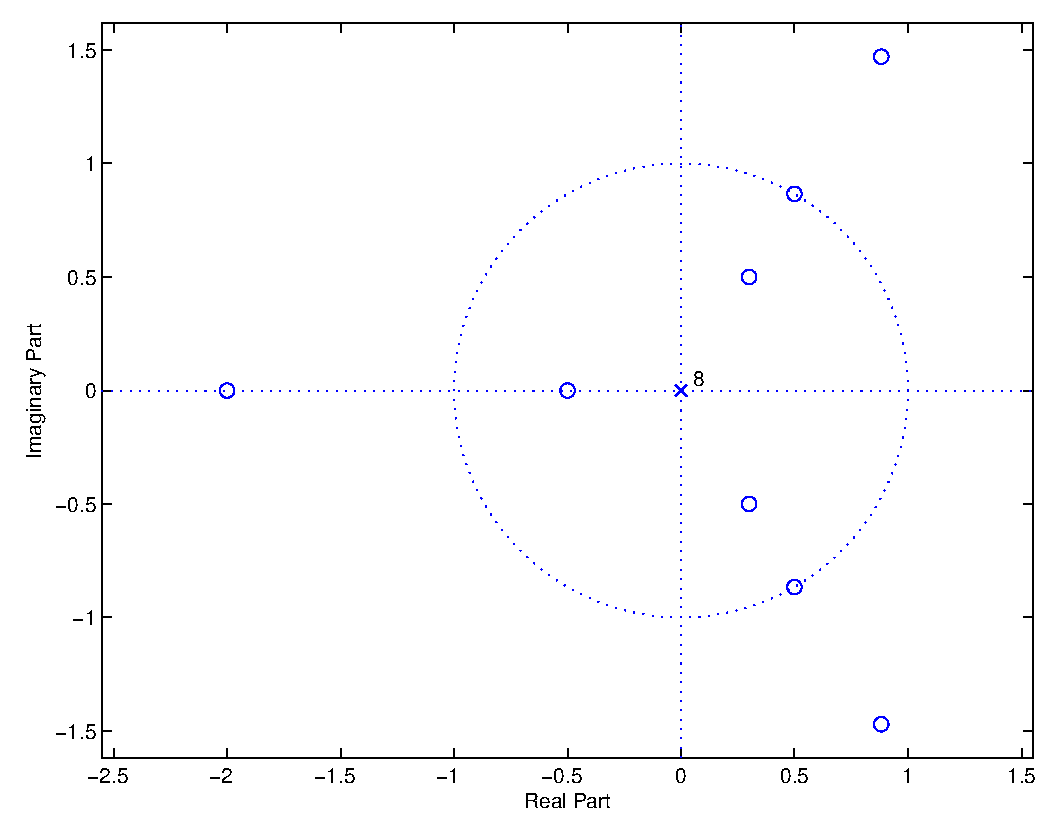
\includegraphics[width=3.8cm]{./Figures/EjFaseLineal1.eps}
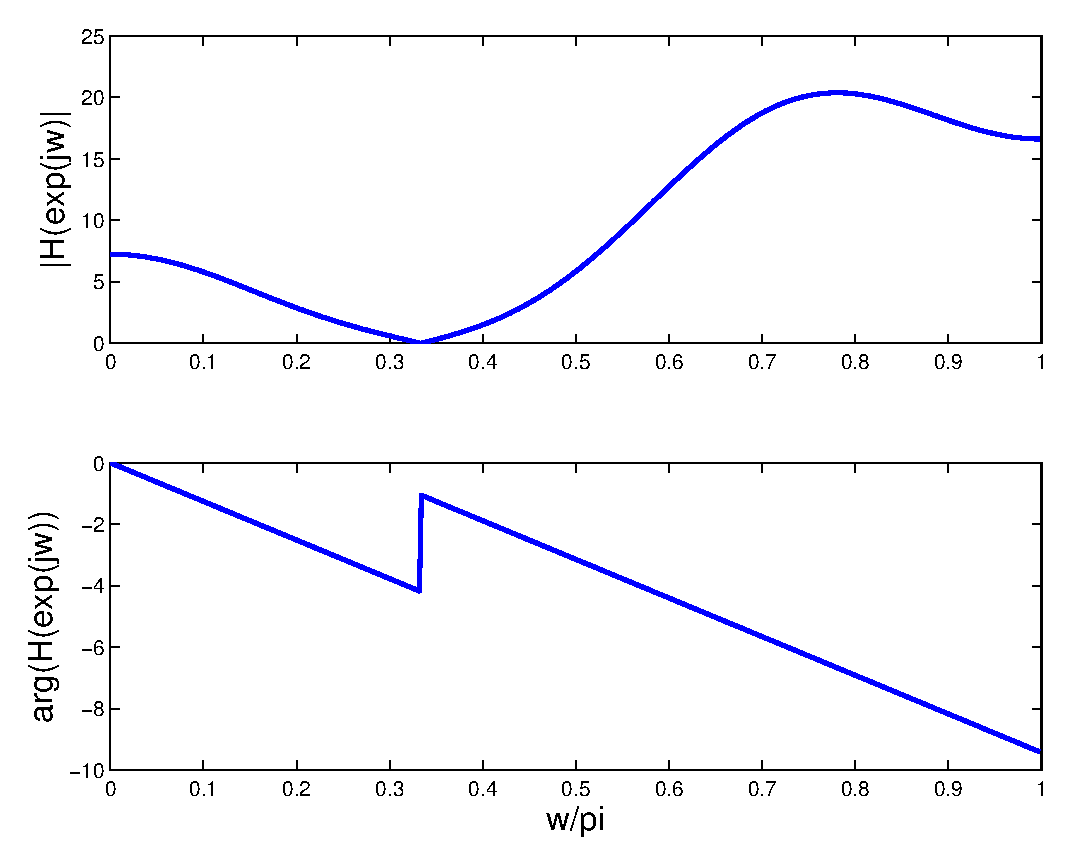
\includegraphics[width=3.8cm]{./Figures/EjFaseLineal2.eps}
\end{column}
\end{columns}





\end{frame}





%%%%%%%%%%%%%%%%%%%%%%%%%%%%%%%%%%%

\begin{frame}
\frametitle{Filtros de fase mínima/máxima }

\vspace{-0.2cm}



\begin{itemize}
\footnotesize
\item Esta clasificación se basa en la posición de los ceros de un sistema.

\visible<2->{

\item \color{olivegreen}Ejemplo: dos sistemas con el mismo polo y ceros invertidos



\begin{itemize}

\color{gray}
\footnotesize

\item $H_1(z)=\frac{z+b}{z+a}$   con $|a|<1$ y $|b|<1$  $\rightarrow Z_{POLO}=-a$ y  $Z_{CERO}=-b$






\item $H_2(z)=\frac{bz+1}{z+a}$   con $|a|<1$ y $|b|<1$ $\rightarrow Z_{POLO}=-a$ y  $Z_{CERO}=-1/b$


\vspace{0.1cm}

$H_2(z)=\frac{bz+1}{z+a}\frac{z+b}{z+b}=\frac{z+b}{z+a}\frac{bz+1}{z+b}=H_1(z)H_{PasoToda}(z)$

\vspace{0.1cm}

$H_2(e^{jw})=H_1(e^{jw})H_{PT}(e^{jw})$ 

\vspace{0.1cm}

\scriptsize

\hspace{1cm}$\rightarrow |H_2(e^{jw})|=|H_1(e^{jw})||H_{PT}(e^{jw})|=|H_1(e^{jw})|$

\vspace{0.1cm}

\hspace{1cm}$\rightarrow arg(H_2(e^{jw}))=arg(H_1(e^{jw}))+arg(H_{PT}(e^{jw}))=$

\vspace{0.1cm}

\hspace{3.1cm}$=arg(H_1(e^{jw}))-\alpha(w)$ con $0<\alpha(w)<\pi$



\color{black}

\end{itemize}

}

\vspace{-0.3cm}

\visible<3->{

\color{black}

\item Generalización:

\begin{itemize}
\footnotesize
\item $H_{MIN}(z)$: FT causal estable con todos sus ceros dentro del círculo unidad

\item $H_{MAX}(z)$: FT causal estable con todos sus ceros simétricos respecto al círculo unidad y el caso anterior

\item $H_{MAX}(z)=H_{MIN}(z)H_{PasoToda}(z)$ con $H_{PT}(z)$ filtro paso todo estable en base a los ceros de $H_{MIN}(z)$

\item $|H_{MAX}(e^{jw})|=|H_{MIN}(e^{jw})|$


\item $arg(H_{MAX}(e^{jw}))=arg(H_{MIN}(e^{jw}))-\alpha(w)$ con $0<\alpha(w)<N\pi$ y N el número de ceros del filtro.


\end{itemize}


}


\end{itemize}
\end{frame}


\begin{frame}
\frametitle{Ejemplo Filtro Fase  Mínima y Máxima}
\footnotesize

\color{olivegreen} Dado un filtro con polos en 0.5, 0.1+0.3j y 0.1-0.3j, y los ceros en 0.3j, -0.3j y 4, determinar el comportamiento del desfase introducido por el filtro. Determinar los filtros de fase mínima y fase máxima asociados con el filtro.

\vspace{-0.4cm}

\color{gray}

\begin{columns}[c]
\begin{column}{5cm}
\lstinputlisting{./Matlab/EjFaseMinima.m}
\end{column}
\begin{column}{5cm}
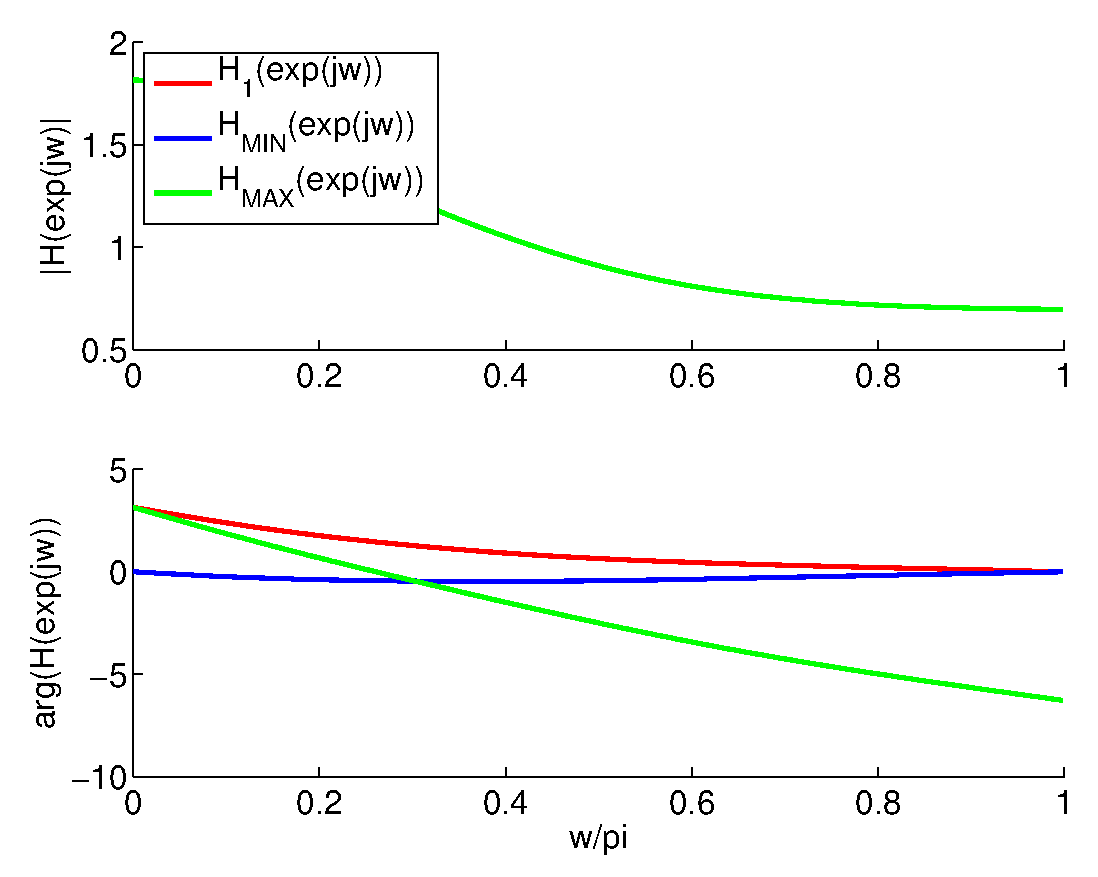
\includegraphics[width=5cm]{./Figures/EjFaseMinima.eps}
\end{column}
\end{columns}

\end{frame}




%%%%%%%%%%%%%%%%%%%%%%%%%%%%%%%%%%%

\begin{frame}
\frametitle{Filtros Combados}

\vspace{-0.2cm}

\begin{itemize}
\footnotesize
\item Son filtros con múltiples bandas de paso y de supresión que tienen una respuesta en frecuencia que es una función periódica en w con periodo $\frac{2\pi}{L}$.
\visible<2->{

\item Se pueden generar a partir de otros filtros discretos G(z) ya diseñados haciendo la transformación $H(z)=G(z^{L})$

\vspace{0.1cm}

$G(z)=\sum_{n=-\infty}^\infty g(n)z^{-n}$

\vspace{0.1cm}

$H(z)=G(z^L)=\sum_{n=-\infty}^\infty g(n)z^{-Ln}$

\vspace{0.1cm}

$H(e^{jw})=\sum_{n=-\infty}^\infty g(n)e^{-jLnw}=G(e^{jwL})$

\item Tenemos una compresión en frecuencia de las características del filtro $G(e^{jw})$. Como la transformada de Fourier en tiempo discreto es periódica en w, la compresión hace que se repita el comportamiento cada $2\pi/L$.

\item Diseño con Matlab de IIR combados:

\begin{itemize}

\item \color{blue}\texttt{[num,den]=iircomb(L,Bw,tipo);}\color{black}

\item Bw: ancho de banda de la comba (normalizado)
\item Tipo: 'peak', 'notch'
\end{itemize}
}





\end{itemize}
\end{frame}


\begin{frame}
\frametitle{Ejemplos de FIR Combados}
\footnotesize

\color{olivegreen} Estudiar la respuesta en frecuencia que se obtiene al combar los siguientes filtros FIR:





\begin{columns}[c]
\begin{column}{4.5cm}

\vspace{0.5cm}


$G_1(z)=\frac{1}{2}(1+z^{-1})$

\vspace{0.2cm}

$G_2(z)=\frac{1}{3}(1+z^{-1}+z^{-2})$

\vspace{1.3cm}




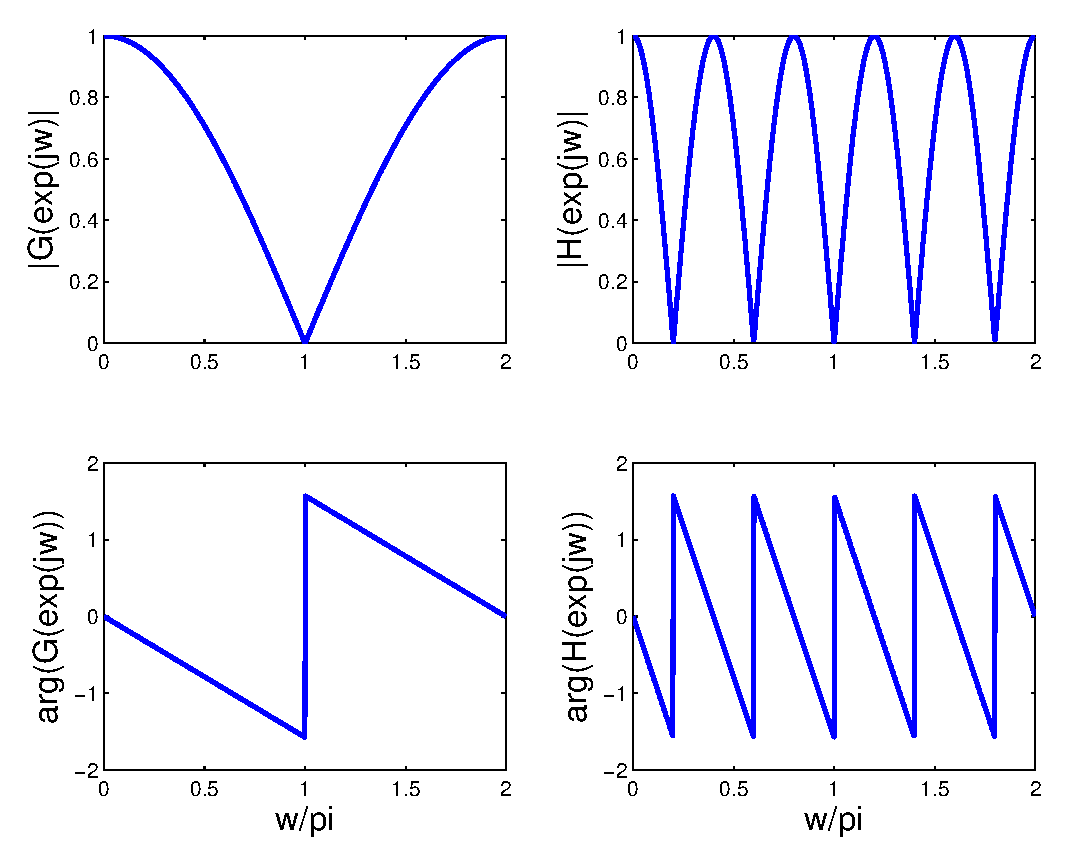
\includegraphics[width=4cm]{./Figures/EjCombFir2.eps}

\color{gray}

\hspace{1.5cm}$G_1(z)$

\end{column}
\begin{column}{5cm}

\color{gray}

\lstinputlisting{./Matlab/EjCombFIR.m}




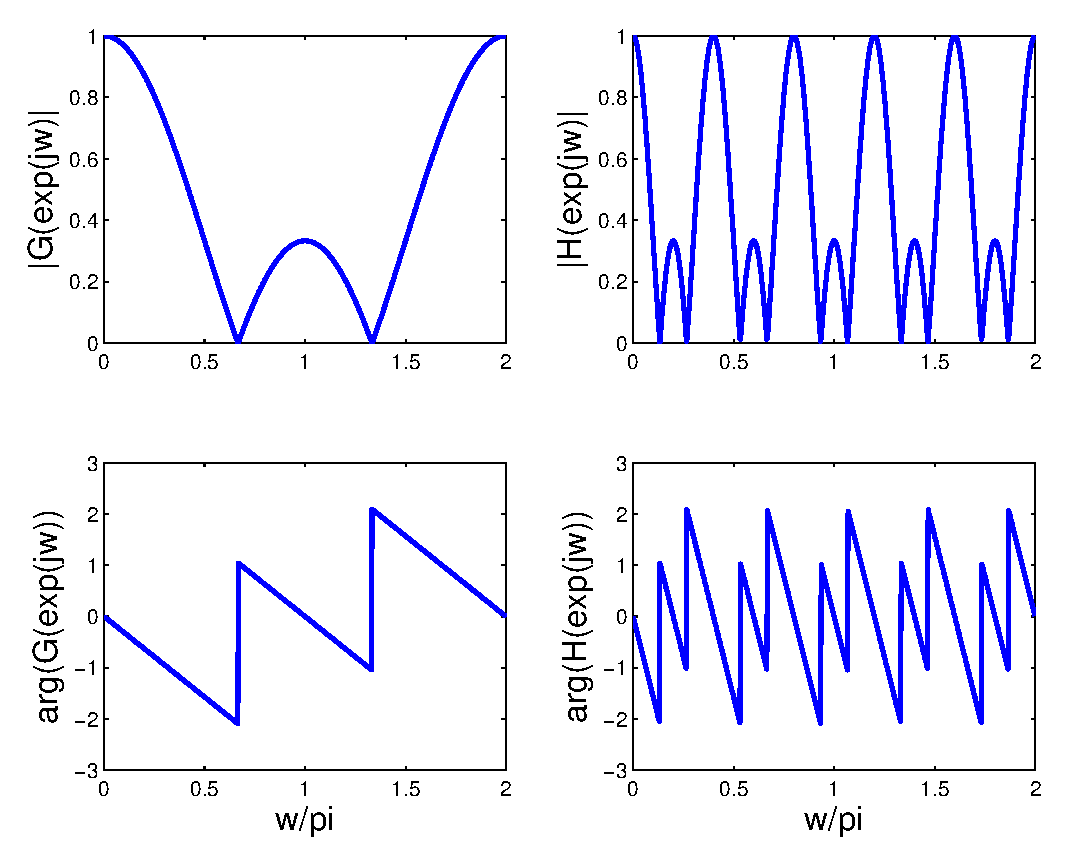
\includegraphics[width=4cm]{./Figures/EjCombFir3.eps}



\hspace{1.5cm}$G_2(z)$

\end{column}
\end{columns}


\end{frame}


%%%%%%%%%%%%%%%%%%%%%%%%%%%%%%%%%%%%%%%%


\begin{frame}
\frametitle{Ejemplos de IIR Combados}
\footnotesize

\color{olivegreen} Estudiar la respuesta en frecuencia que se obtiene al combar el siguiente filtro IIR:





\begin{columns}[c]
\begin{column}{4.5cm}

\vspace{0.5cm}


$G(z)=0.4\frac{1-z^{-1}}{1+0.2z^{-1}}$

\color{gray}

\lstinputlisting{./Matlab/EjCombIIR.m}



\end{column}
\begin{column}{5cm}

\color{gray}



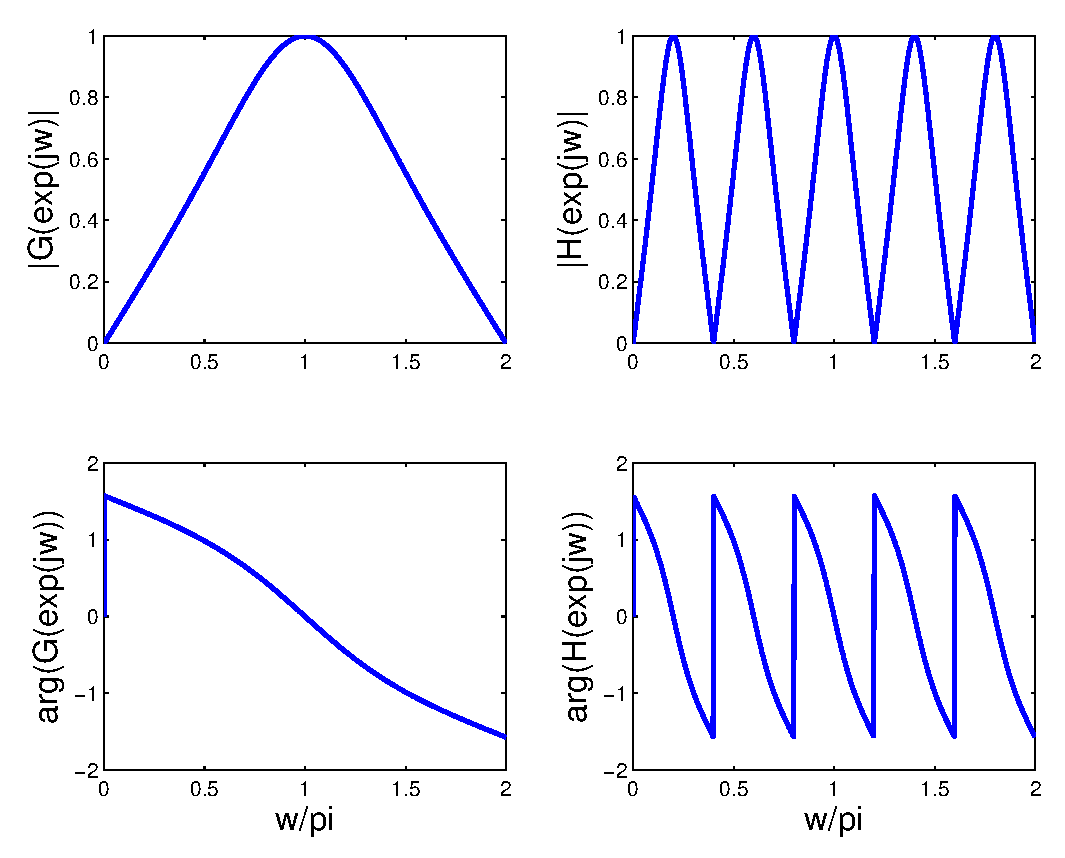
\includegraphics[width=4cm]{./Figures/EjCombIIR.eps}



\end{column}
\end{columns}


\end{frame}


%%%%%%%%%%%%%%%%


\begin{frame}
\frametitle{Ejemplos de IIR Combados con Matlab}
\footnotesize

\color{olivegreen} Diseñar un filtro combado para eliminar la f=15Hz y sus múltiplos para un sistema muestreo a f=300Hz.


\begin{columns}[c]
\begin{column}{4.5cm}

\vspace{0.5cm}

\color{gray}

$w_d=w_cT_s=2\pi \frac{f_{eliminar}}{f_s}=\frac{2\pi}{L}  \rightarrow L=\frac{f_s}{f_{eliminar}}=20$

$B_{w,max}=\frac{2\pi}{L}=0.314$

\lstinputlisting{./Matlab/EjCombIIRMatlab.m}



\end{column}
\begin{column}{5cm}

\color{gray}



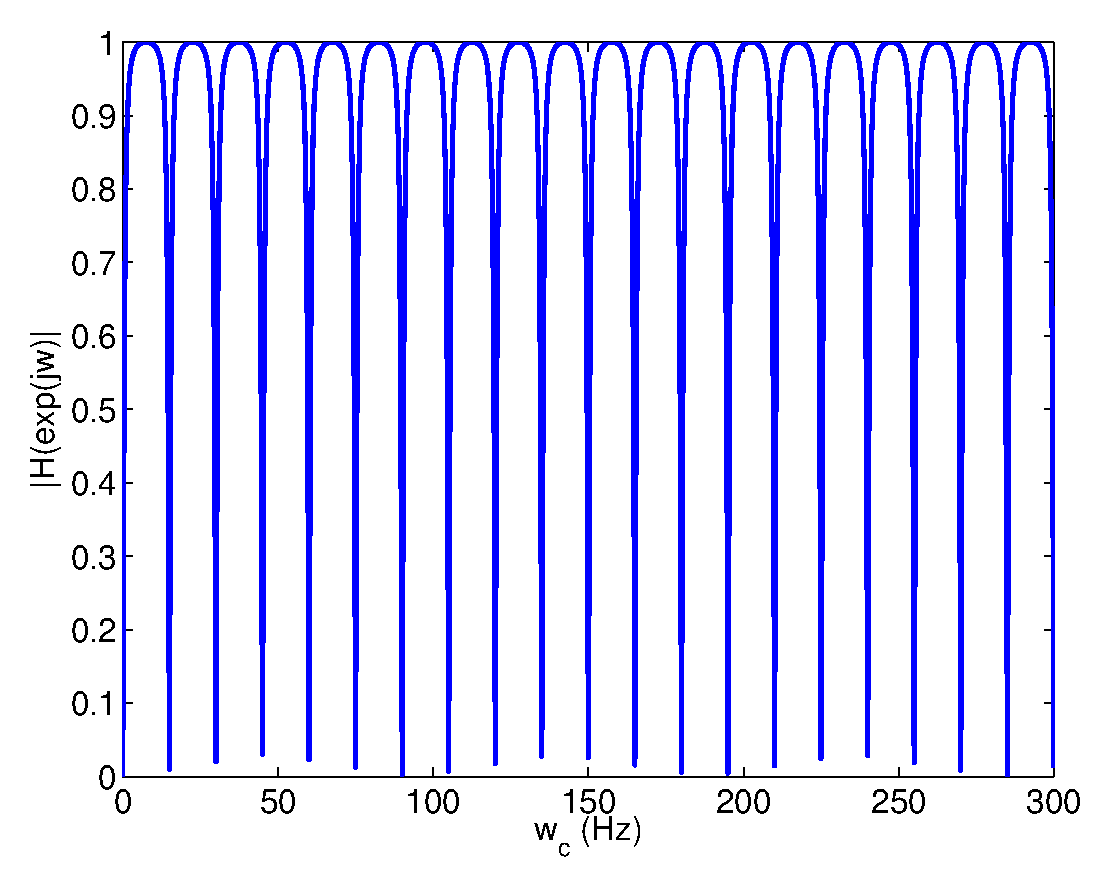
\includegraphics[width=4cm]{./Figures/EjCombIIRMatlab.eps}



\end{column}
\end{columns}


\end{frame}





\begin{frame}
  \frametitle{Conceptos Importantes}
  \begin{itemize}
    \item \alert{¿Cómo especificar un filtro paso bajo?}
    \begin{itemize}
      \item $\color{blue}(\omega_p,\omega_s)$ Frecuencias de paso y supresión.
      \item $\color{blue}(\alpha_p,\alpha_s)$ Atenuación máxima de paso y mínima de supresión.
    \end{itemize}
    
    \item \alert{Algunos tipos de filtros continuos}
    \begin{itemize}
      \item Butterworth (respuesta plana),
      \item Chebyshev Tipo I (rizado en banda de paso).
      \item Chebyshev Tipo II (rizado en banda de supresión).
      \item Elíptico (rizado en banda de paso y supresión).
    \end{itemize}

    \item \alert{¿Y para filtros paso alto, paso banda y supresor de banda?}
    \begin{itemize}
      \item Transformación espectral
    \end{itemize}
  \end{itemize}
  
\end{frame}

\end{document}
